\documentclass{beamer}
\usepackage{graphicx}
\usepackage[english]{babel}
\usepackage{etoolbox}
\usepackage{wasysym}
\usepackage[autostyle, english=american]{csquotes}
\MakeOuterQuote{"}

\graphicspath{{images/}{plots/}}

\title{Effect of Strong Stellar Interactions on Planetary Systems and
            the Formation of Hot Jupiters}
\author{Tyler Reisinger}
\date{}

\begin{document}
\setbeamertemplate{caption}{\raggedright\insertcaption\par}
\setbeamerfont{caption}{size=\scriptsize}
\addtobeamertemplate{navigation symbols}{}{ \hspace{1em}    \usebeamerfont{footline}%
    \insertframenumber / \inserttotalframenumber }

\begin{frame}
    \maketitle
    \begin{center}
        Advisor: Dr. Steve McMillan
    \end{center}
    \begin{figure}
        \centering
        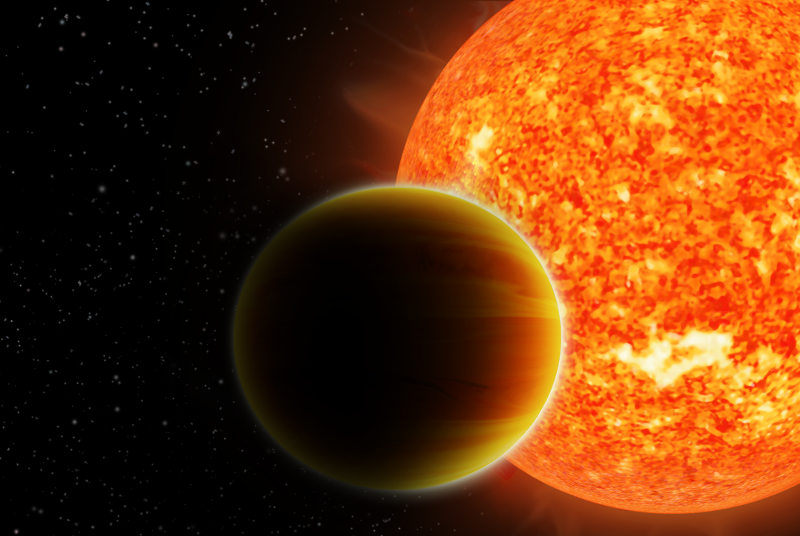
\includegraphics[height=1.25in]{Image1_HotJupiter1}
    \end{figure}
\end{frame}

\begin{frame}{Overview}
    \tableofcontents
\end{frame}

\section{Background}

\begin{frame}{Hot Jupiters}
    \begin{columns}
        \column{0.66\textwidth}
            \begin{itemize}
                \item Jupiter-mass planets orbiting very close ($<0.5$ AU) to their host star.
                \item Jupiters are believed to form far out in the solar system.
                    \begin{itemize}
                        \item How do they become so close?
                        \item What causes their migration?
                    \end{itemize}
                \item An estimated 1\% of planetary systems contain a 
                    Hot Jupiter (A. Brucalassi et al. 2016)\footnotemark.
            \end{itemize}
        \column{0.34\textwidth}
            \begin{figure}
                \centering
                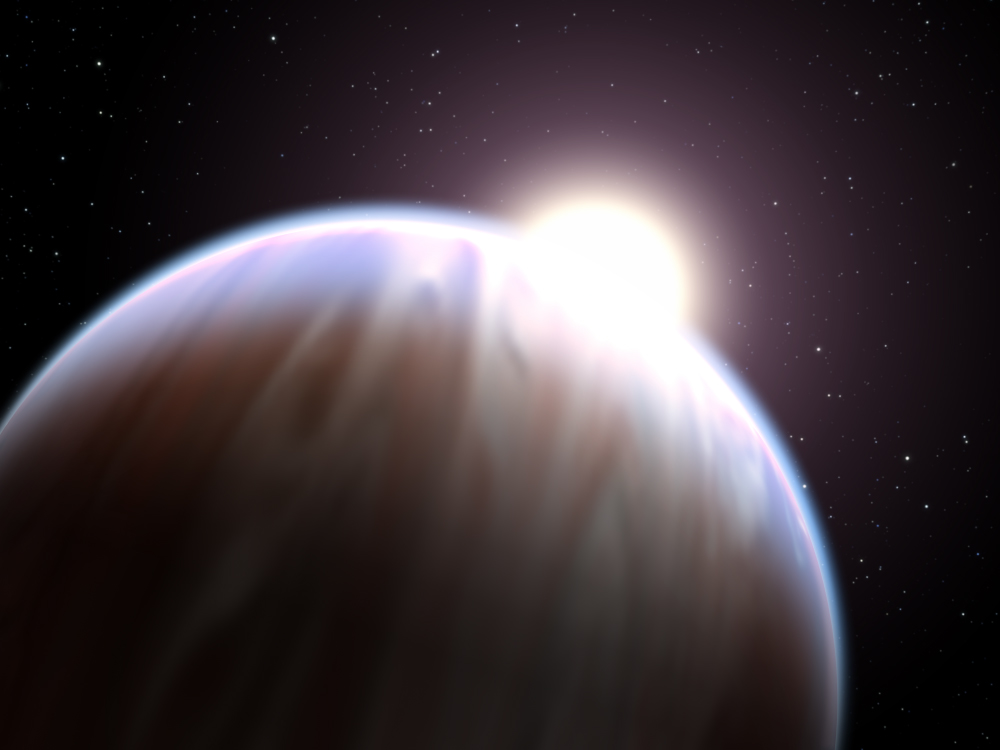
\includegraphics[width=1.66in]{large_hj}
            \end{figure}
    \end{columns}

    \footnotetext[1]{James B. Pollack, Olenka Hubickyj, Peter Bodenheimer, Jack J. Lissauer, Morris Podolak, Yuval Greenzweig, Formation of the Giant Planets by Concurrent Accretion of Solids and Gas, Icarus, Volume 124, Issue 1, 1996, Pages 62-85, ISSN 0019-1035, http://dx.doi.org/10.1006/icar.1996.0190.
(http://www.sciencedirect.com/science/article/pii/S0019103596901906) }

\end{frame}

\begin{frame}{Background}
    \begin{columns}
        \column{0.66\textwidth}
        \begin{itemize}
            \item Explore formation scenarios for Hot Jupiters (HJs) in planetary
                systems.
            \item Understand the side-effects of HJ formation.
                \begin{itemize}
                    \item Does the migration of the HJ affect other planetary orbits?
                    \item Are terrestrial planets in highly eccentric orbit a possible
                        indicator of Hot Jupiter formation?
                \end{itemize}
        \end{itemize} 
        \column{0.34\textwidth}
            \begin{figure}
                \centering
                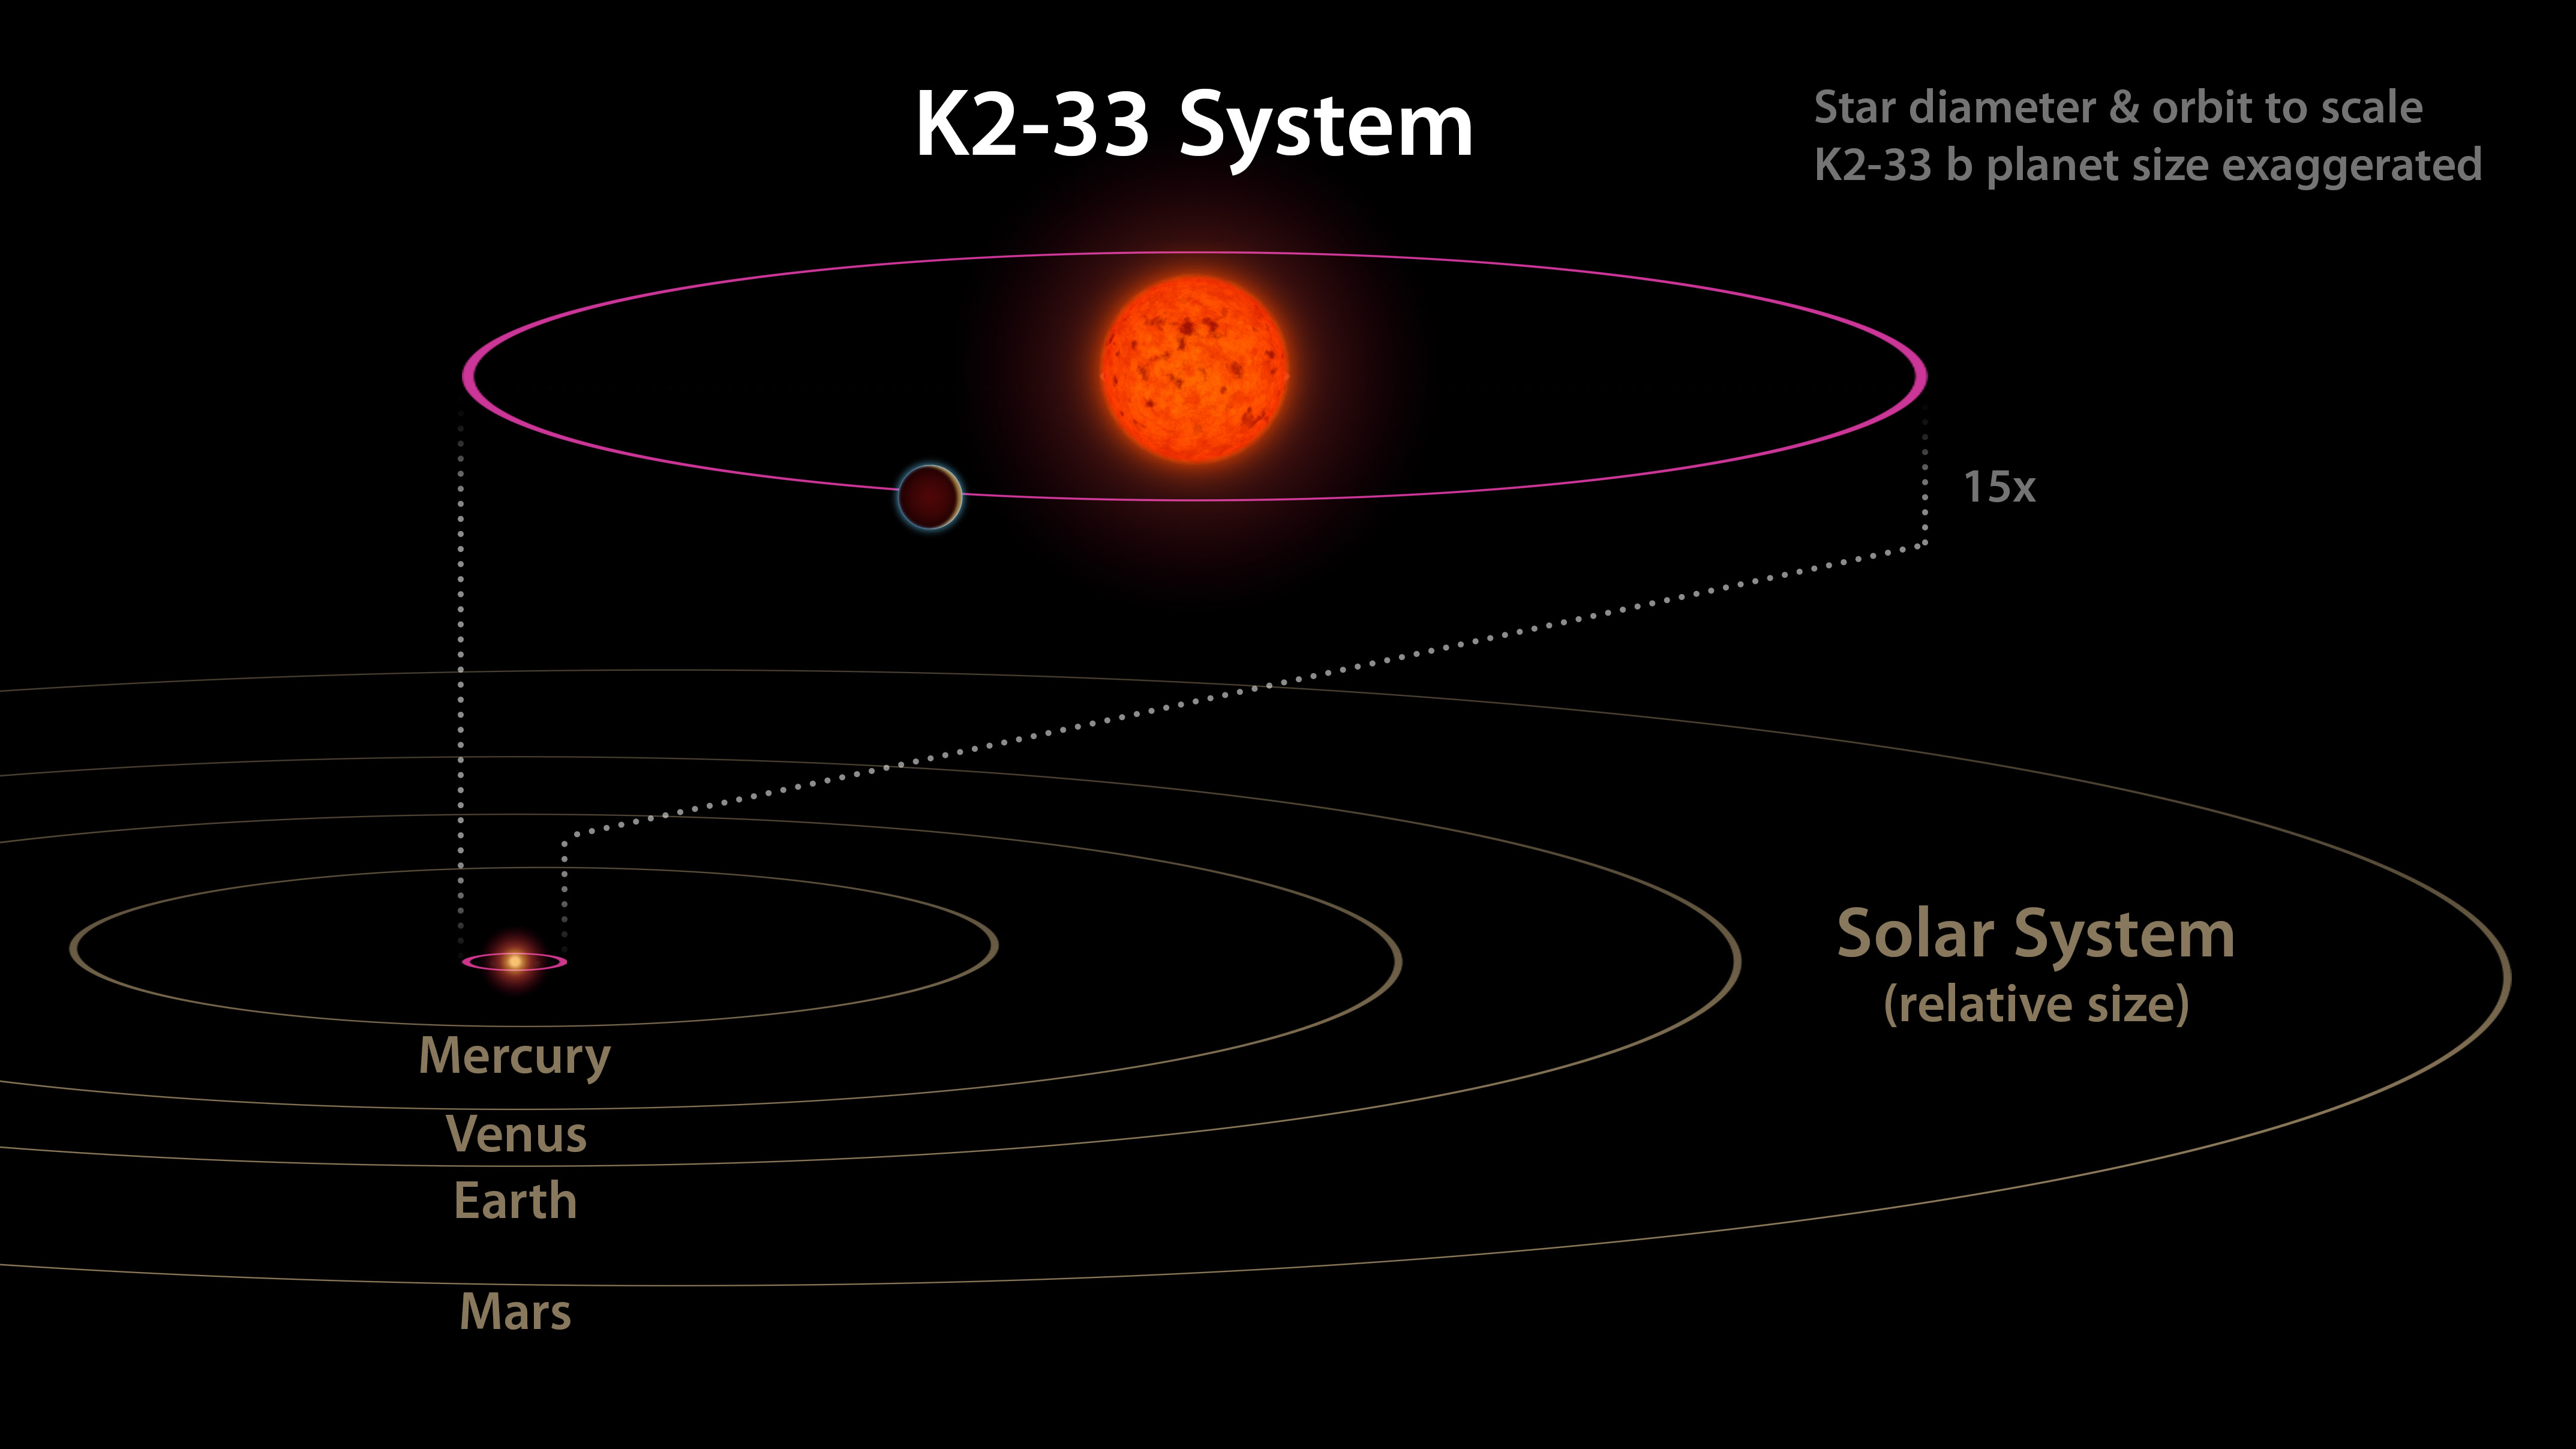
\includegraphics[width=1.66in]{hj_orbit}
            \end{figure}
    \end{columns}
\end{frame}

\begin{frame}{Theory}
    \begin{columns}
        \column{0.67\textwidth}
        \begin{itemize}
            \item Scattering Effects
                \begin{itemize}
                    \item HJs start like normal gas planets, but are perturbed inward.
                    \item Perturbation may come from stellar interactions
                        within a star cluster.
                    \item This could cause other planets in the system to be
                        knocked into eccentric orbits by the HJ.
                        \begin{itemize}
                            \item If we understand what this might look like,
                                we can look for it in the universe.
                        \end{itemize}
                \end{itemize}
            \item We will use computational simulations to explore this scenario.
        \end{itemize}
        \column{0.33\textwidth}
            \begin{figure}
                \centering
                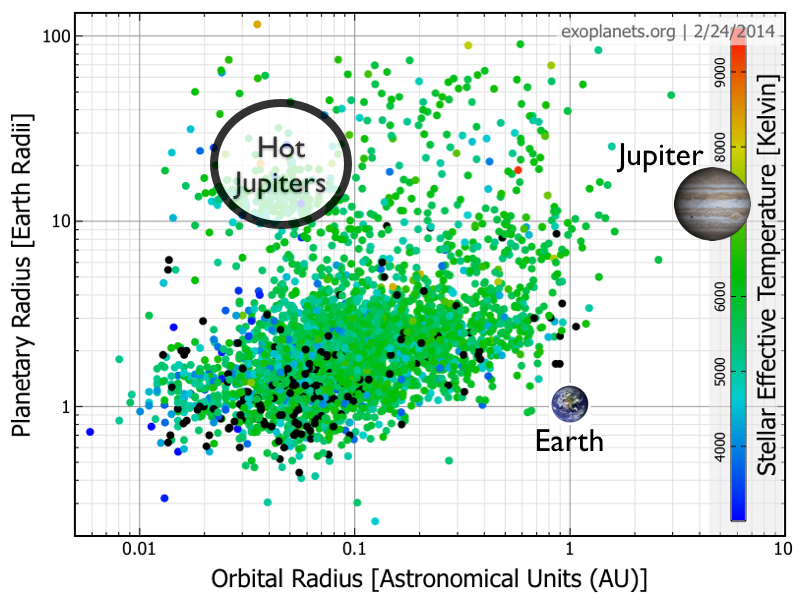
\includegraphics[height=1.25in]{hot_jupiter_measure_plot}
            \end{figure}
    \end{columns}
\end{frame}

\begin{frame}{Orbital Elements}
    \begin{itemize}
        \item Allow us to compute the closest approach analytically.
        \item Characterize planetary orbits.
        \item Allow numerical categorization of orbit changes.
    \end{itemize}
    \begin{figure}
        \centering
        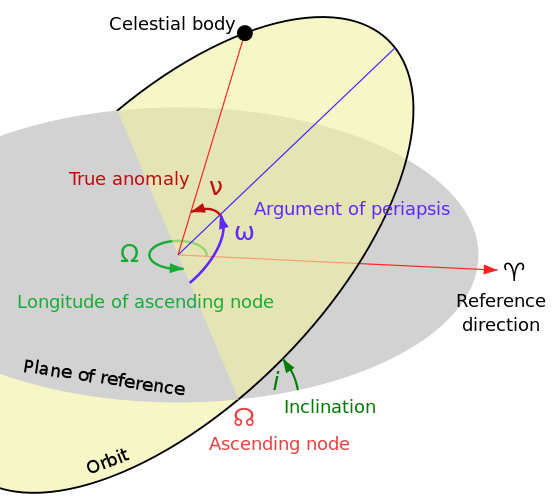
\includegraphics[height=1.5in]{orbital_elems}
    \end{figure}

\end{frame}

\begin{frame}{Orbital Elements}
    \begin{description}
        \item[e] -- Eccentricity - How oblong the orbit is.
            \begin{itemize}
                \item $e = 0.0$ is a circular orbit.
                \item $e < 1.0$ is an elliptical orbit.
                \item $e > 1.0$ is a hyperbolic escape trajectory.
            \end{itemize}
        \item[a] -- Semimajor Axis - The longest orbital axis length.
        \item[i] -- Inclination - Vertical tilt from horizontal.
    \end{description}
    \begin{figure}
        \centering
        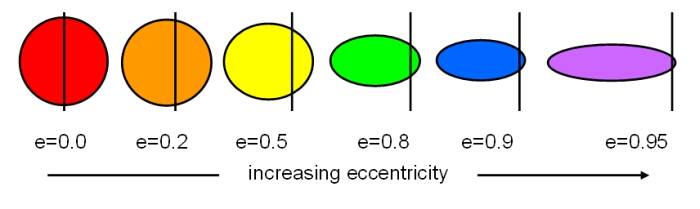
\includegraphics[height=1.2in]{eccentricity}
    \end{figure}
\end{frame}

\begin{frame}{Periapsis}
    \begin{itemize}
        \item Periapsis -- The point of closest approach of two orbiting bodies.
        \item Distance at periapsis is distance of closest approach.
        \item Easily computed from orbital elements:
            \begin{equation}
                r_{per} = (1 - e) a
            \end{equation}
    \end{itemize}
    \begin{figure}
        \centering
        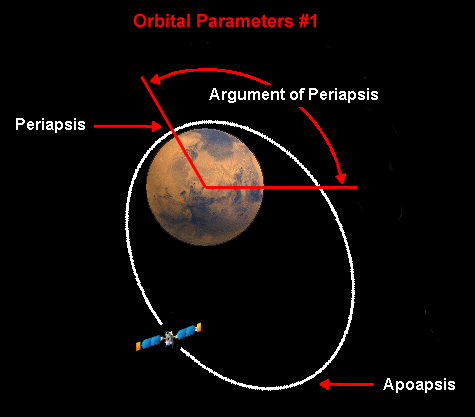
\includegraphics[height=1.75in]{periapsis_diag}
    \end{figure}
\end{frame}

\section{Methods}

\begin{frame}{Environment \& Code}
    \begin{itemize}
        \item Simulations are built atop the AMUSE astrophysics library.
        \item Run on Drexel's Draco computing cluster.
        \item 24 node shared between all users.
        \begin{itemize}
            \item Three to six GPUs on each node
            \item 12 core CPUs
        \end{itemize}
        \begin{figure}
            \centering
            \begin{tabular}{cc}
                
\includegraphics[height=1in]{AmuseLogo} & 
\includegraphics[height=1in]{PythonLogo}
            \end{tabular}
        \end{figure}
    \end{itemize}
\end{frame}

\begin{frame}{Simulation Framework}
    \begin{itemize}
        \item AMUSE does the gravitational dynamics in highly efficient code.
        \item Our python code sits on top
        \begin{itemize}
            \item Setup the simulation initial state
            \item Send the full setup to AMUSE
            \item Let AMUSE run the simulation
            \item Periodically pause the simulation to observe the state
                \begin{itemize}
                    \item AMUSE may also send us notifications about close encounters
                        as it runs.
                \end{itemize}
        \end{itemize}
    \end{itemize}
\end{frame}

\begin{frame}{Star Cluster Simulation}
    \begin{itemize}
        \item Jupiter-mass planets are only affected by very close ($\le $30 AU) encounters.
        \item Time scale between these interactions is long.
            \begin{itemize}
                \item About 1 encounter per 0.1 Myr
                \item Not all of these are interesting for planetary interactions.
            \end{itemize}
        \item Time scale for planetary orbits are short.
            \begin{itemize}
                \item Earth orbits the sun in 0.001 Myr.
            \end{itemize}
        \item Simulating planets in the cluster would require much more
            computation than just stars.
    \end{itemize}
    \begin{figure}
        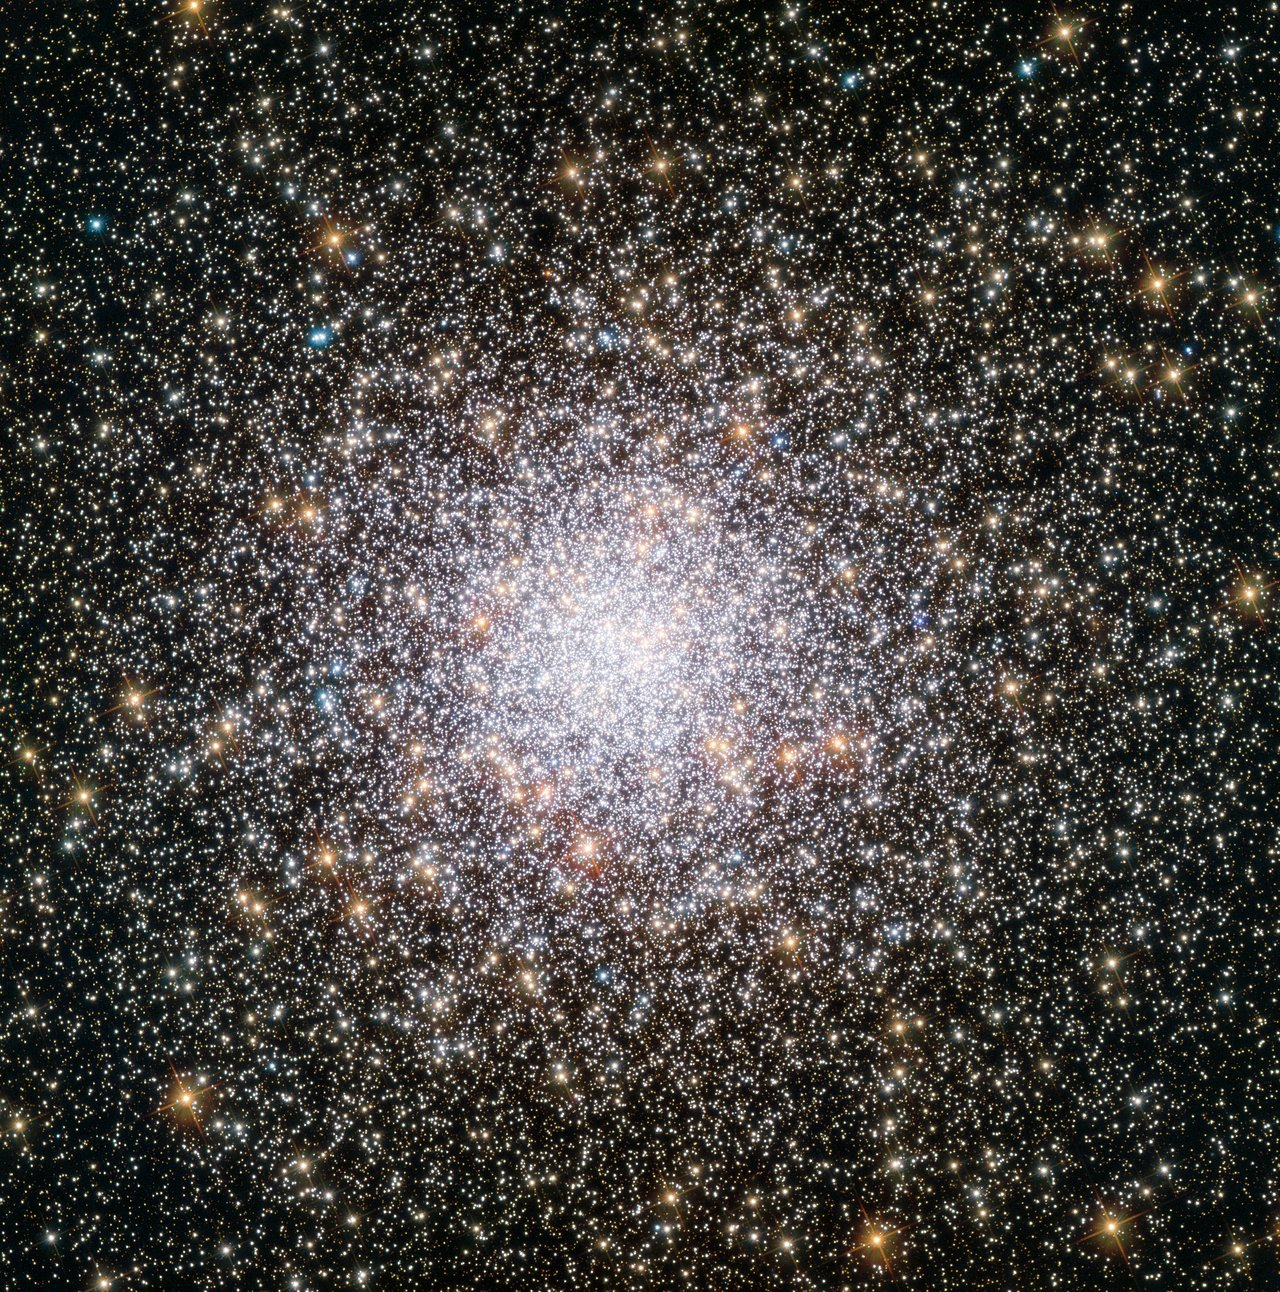
\includegraphics[height=1.5in]{star_cluster.jpg}
    \end{figure}
\end{frame}

\begin{frame}{Star Cluster Simulation}
    Idea: Simulate only stars and add planets later in isolation.
    \begin{itemize}
        \item Record exact parameters of star encounters.
        \item Don't waste resources simulating stable planet orbits.
        \item Allows much more detailed simulation for strong encounters
            without slowing everything down.
        \item The data can be reused with different configurations of planets.
    \end{itemize}
\end{frame}

\begin{frame}{Data Pipeline}
    \begin{enumerate}
        \item Star Cluster N-Body simulations
            \begin{itemize}
                \item Catalog close encounters for later simulation
            \end{itemize}
        \item Planetary system simulations of two interacting systems.
            \begin{itemize}
                \item Use encounters found in star cluster simulations.
                \item Observe how these encounters affect planets.
                \item Save planetary system end-states for analysis.
            \end{itemize}
        \item Analysis 
            \begin{itemize}
                \item Observe patterns over many different encounters.
                \item Look for Hot Jupiter formation or other interesting events.
            \end{itemize}
    \end{enumerate}
\end{frame}

\section{Pipeline}

\begin{frame}{Star Cluster Simulation Approach}
    \begin{itemize}
        \item Run many gravitational simulations of star clusters.
            \begin{itemize}
                \item Each cluster has the same set of parameters.
                \begin{itemize}
                    \item Number of Stars
                    \item Mass distribution
                \end{itemize}
            \end{itemize}
        \item Catalog encounter parameters of all close star-star encounters.
        \begin{figure}
            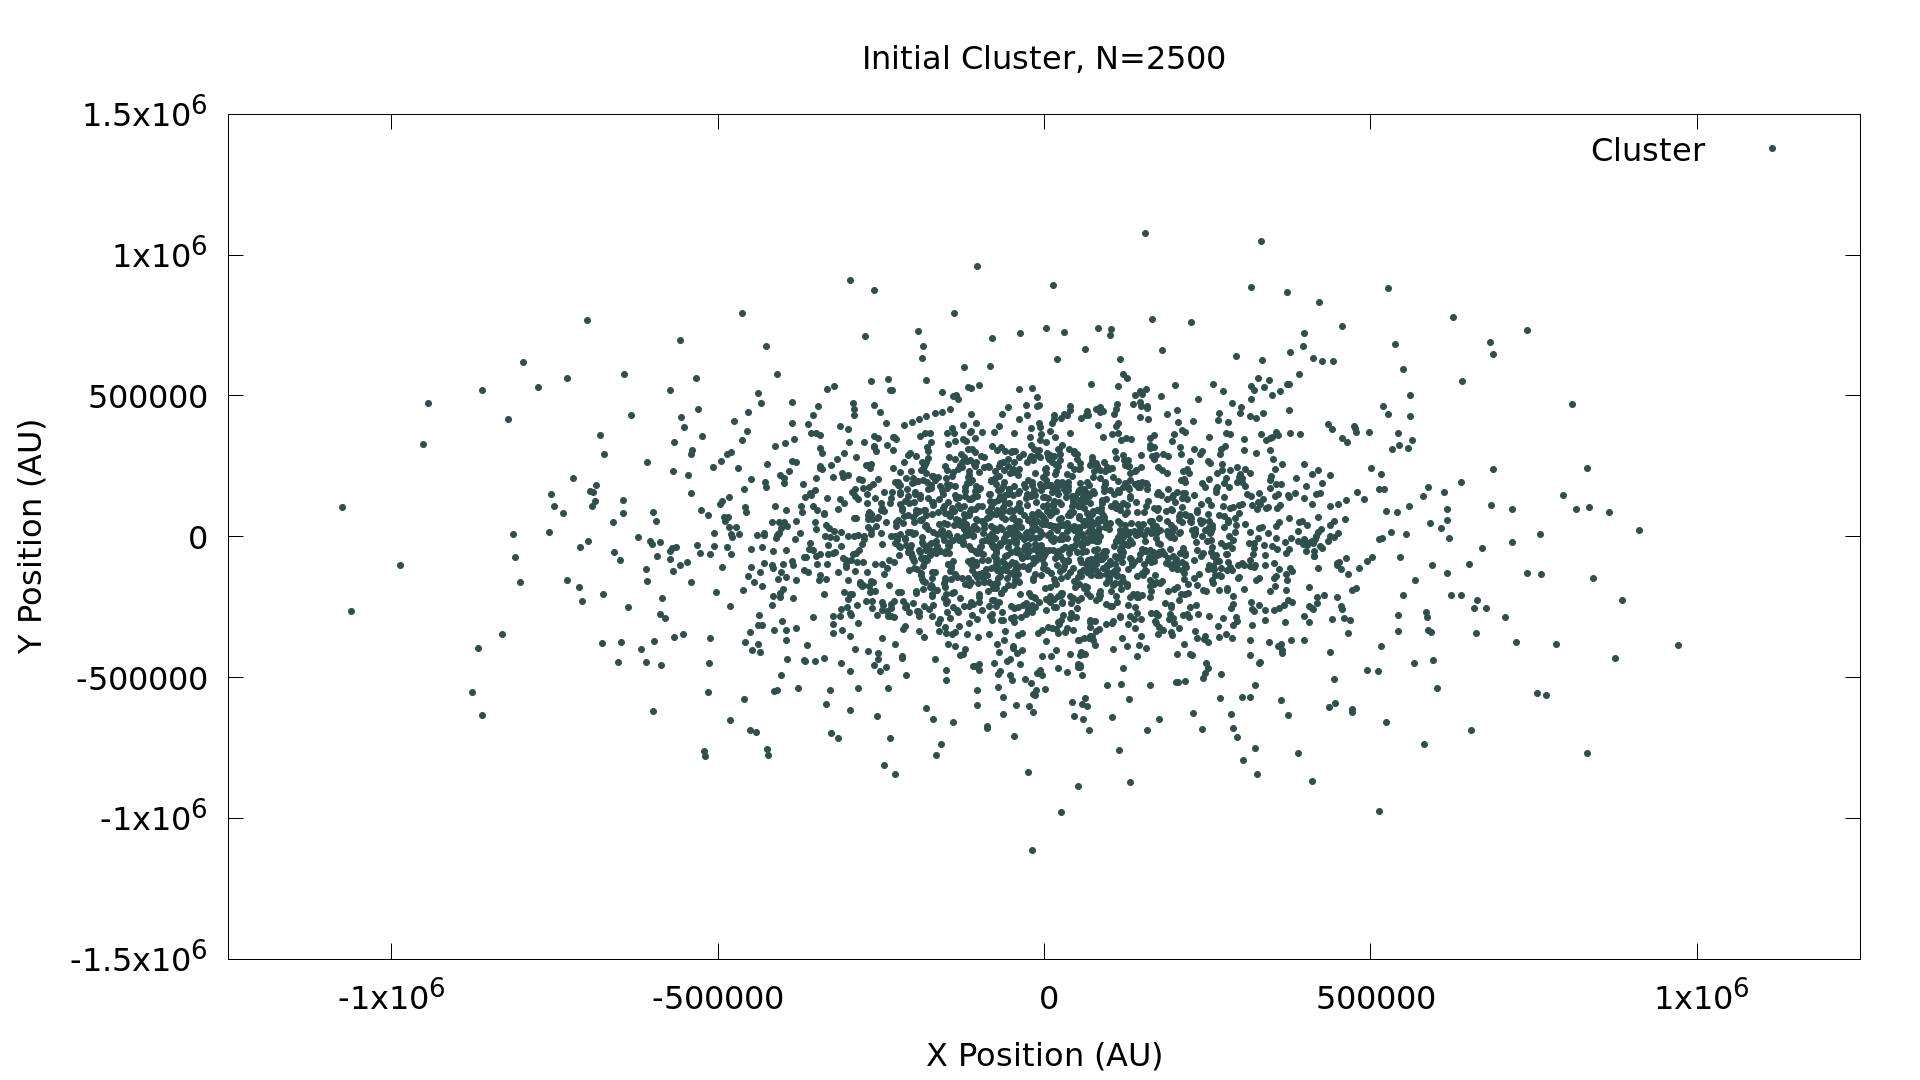
\includegraphics[height=1.5in]{cluster1.png}
        \end{figure}
    \end{itemize}
\end{frame}

\begin{frame}{Star Cluster Setup}
    \begin{itemize}
        \item King Model with $W_0 = 3.0$.
            \begin{itemize}
                \item Sampled randomly to create a cluster.
            \end{itemize}
        \item Clusters of 1000, 2000 and 4000 stars.
        \item Run for 250, 500, 1000 Myr, respectively.
        \item Each star has fixed $M = 1 M_{\astrosun}$.
    \end{itemize}
    \begin{figure}
        \centering
        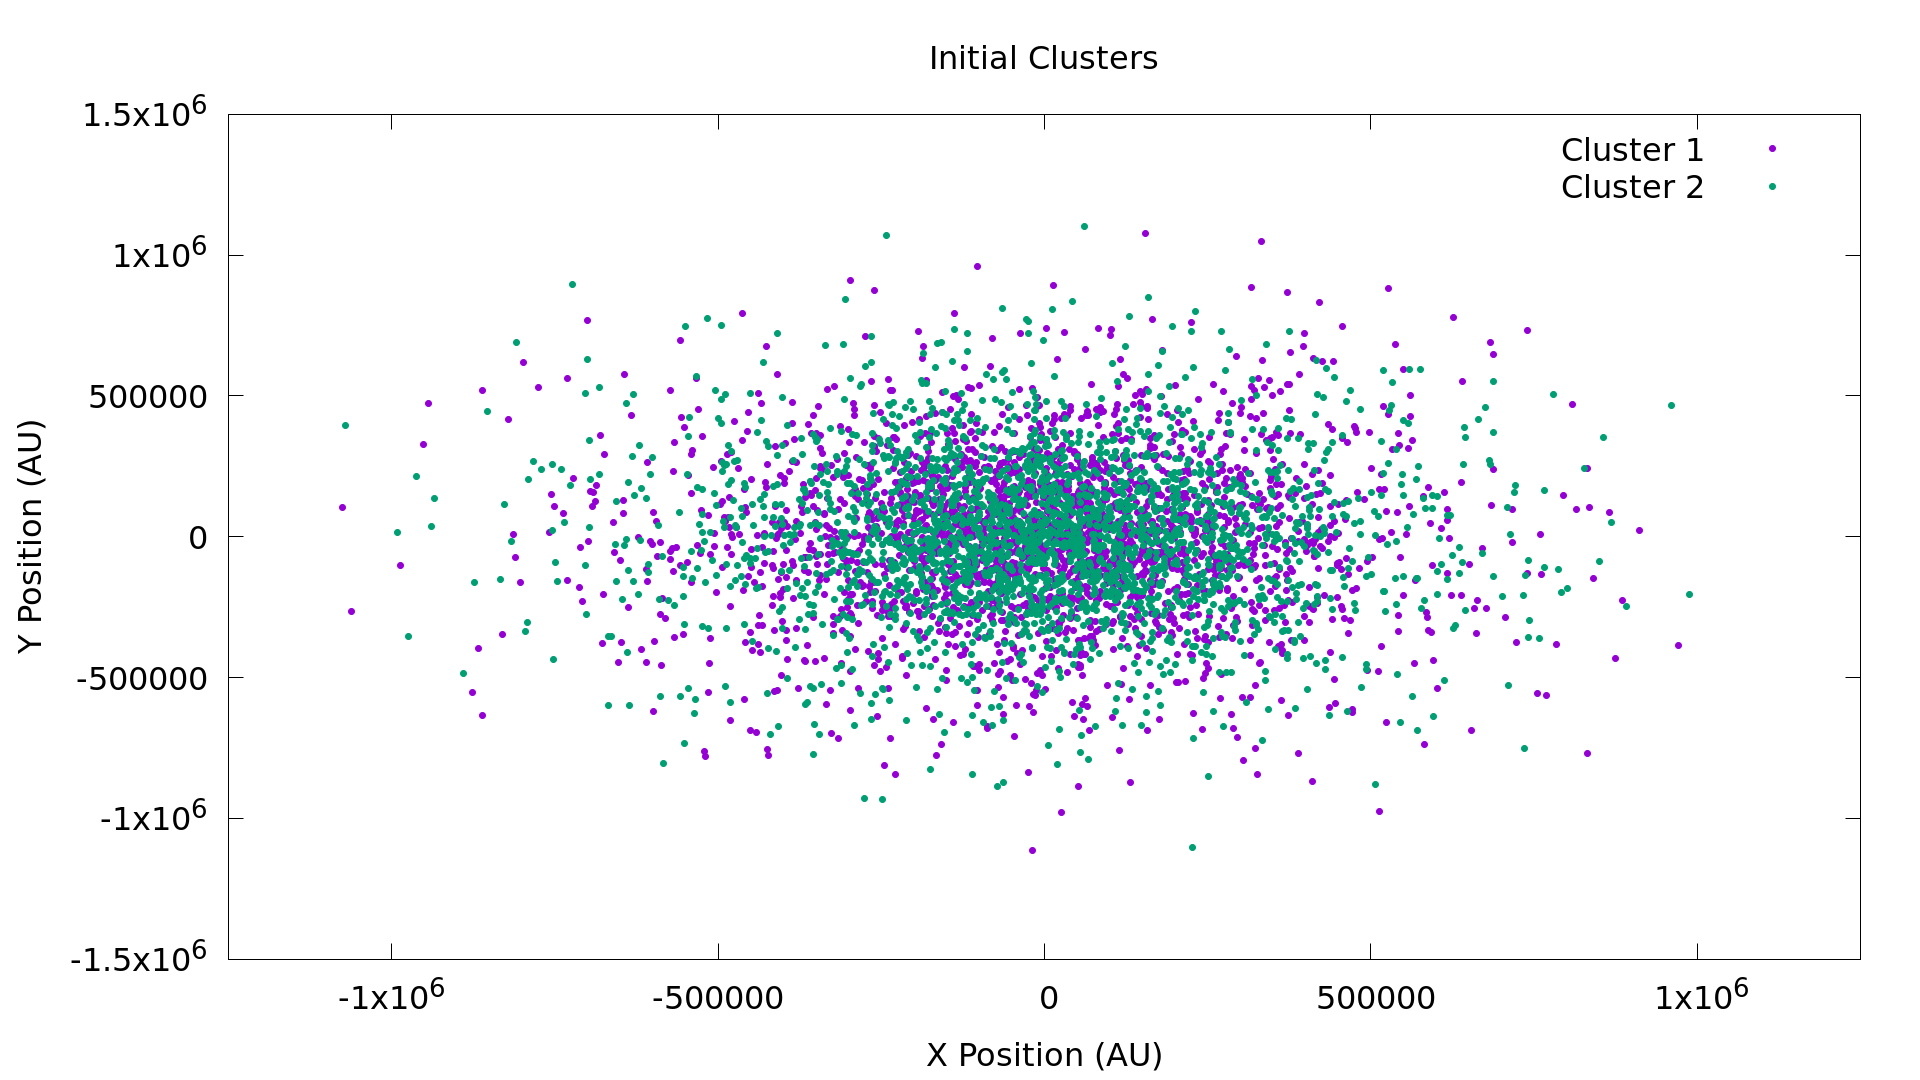
\includegraphics[height=1.5in]{cluster_superimposed.png}
    \end{figure}
\end{frame}

\begin{frame}{Star Cluster Simulation}
    \begin{itemize}
        \item Let AMUSE simulate a cluster, call back into user code for close
            stellar encounters.
        \item Compute and record:
            \begin{itemize}
                \item Dynamical parameters of each star.
                \item Orbital parameters $(a, e, r)$
                \item Distance of closest encounter
            \end{itemize}
    \end{itemize}
    \begin{figure}
        \begin{tabular}{cc}
            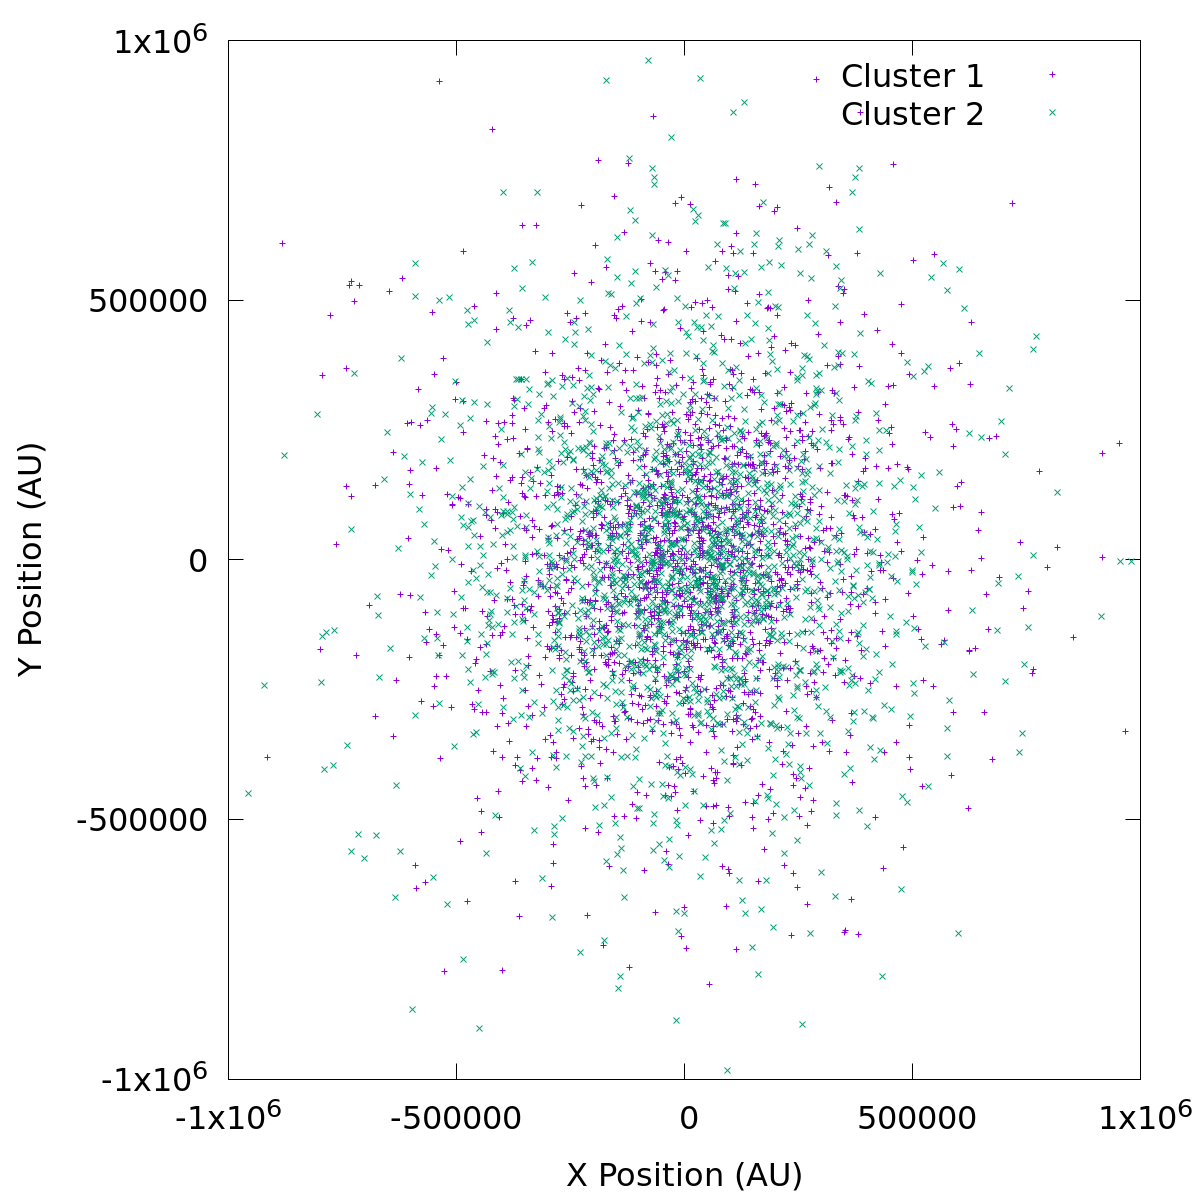
\includegraphics[height=2.0in]{clusters_superimposed_n_2000} &
            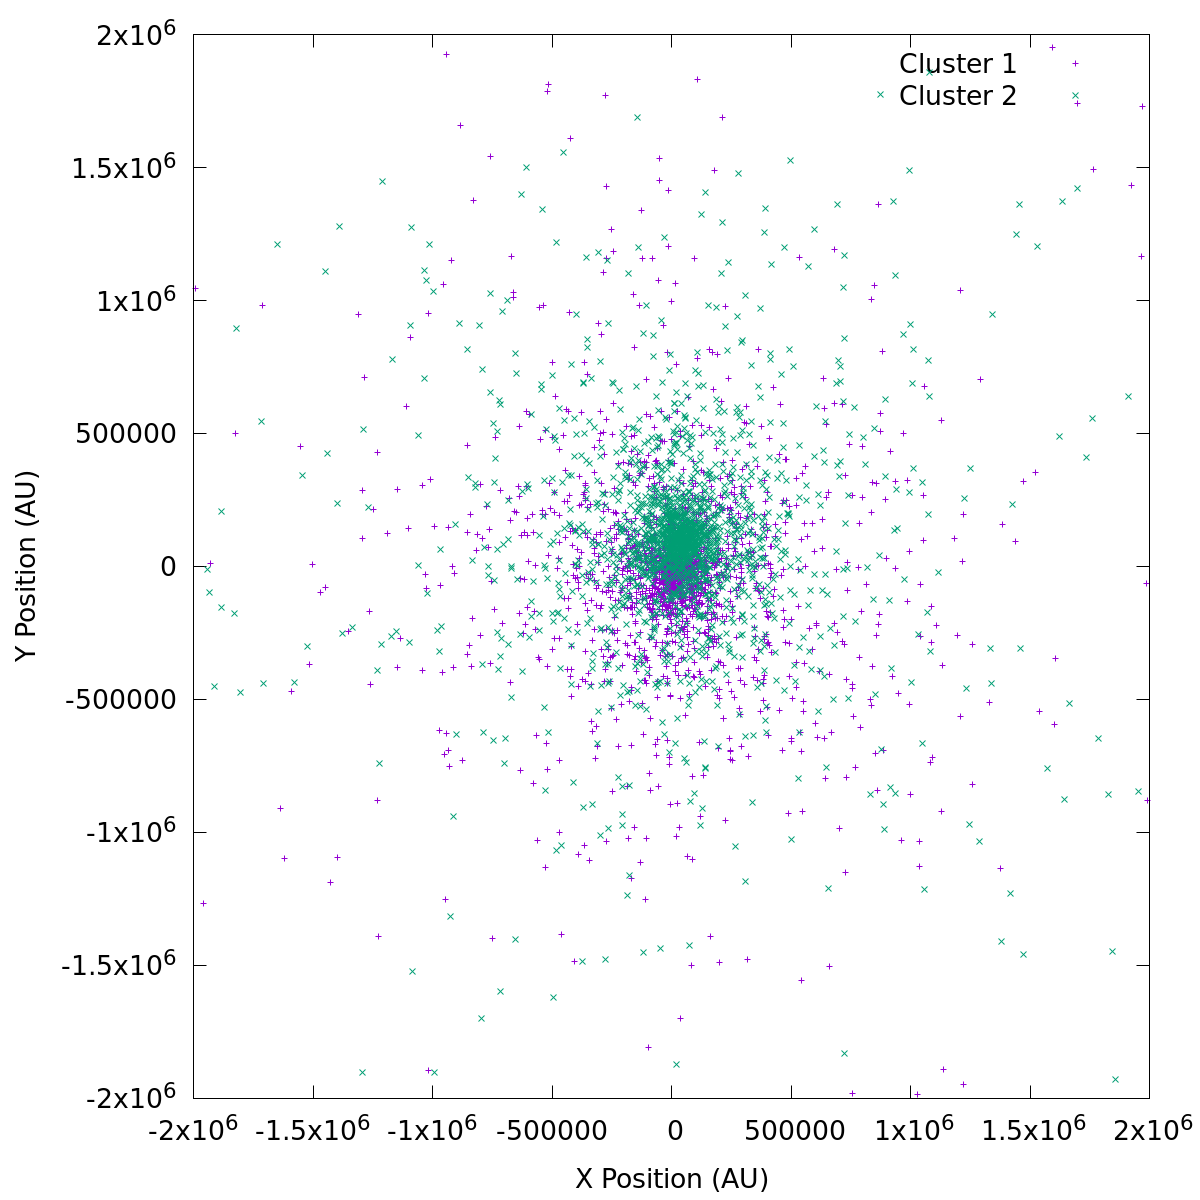
\includegraphics[height=2.0in]{clusters_superimposed_final_n_2000}
        \end{tabular}
    \end{figure}
\end{frame}

\begin{frame}{Encounters}
    \begin{columns}
        \column{0.5\textwidth}
            \begin{itemize}
                \item For 1000 star clusters...
                    \begin{itemize}
                        \item 1,000 total clusters simulated.
                        \item 250 Myr each.
                        \item 1,831,075 encounters returned between 0 and 500 AU periastron.
                        \item 57,351 encounters at 30 AU or less.
                            \begin{itemize}
                                \item This is the most distant approach considered for Jupiters.
                            \end{itemize}
                    \end{itemize}
            \end{itemize}
        \column{0.5\textwidth}
            \begin{figure}
                \centering
                \caption{Histogram of closest approach distance of two stars in 1000 star cluster.}
                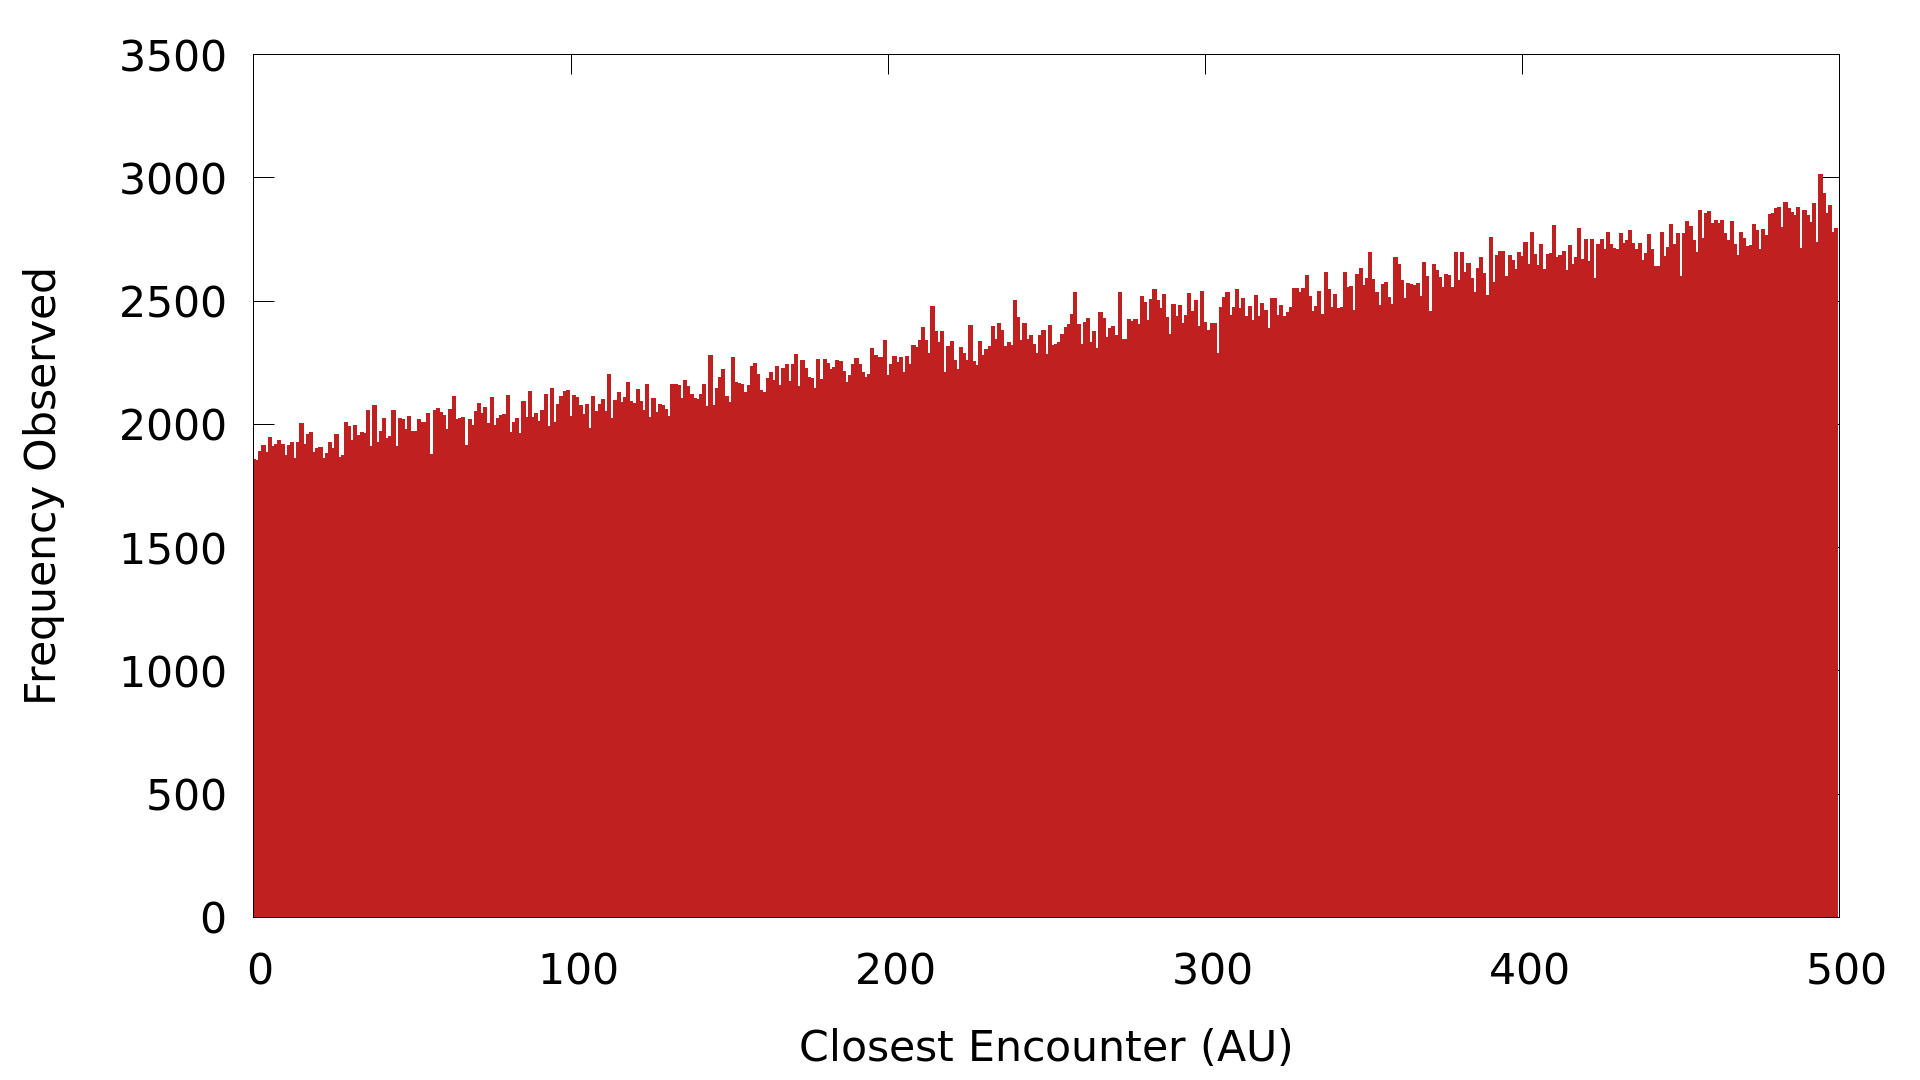
\includegraphics[width=2.25in]{encounter_distance_frequency_n1000}
            \end{figure}
    \end{columns}
\end{frame}

\begin{frame}{Encounters}
    \begin{itemize}
        \item For clusters with more stars, close encounters were more frequent.
    \end{itemize}
    \begin{figure}
        \centering
        \caption{1000 vs 4000 star clusters}
        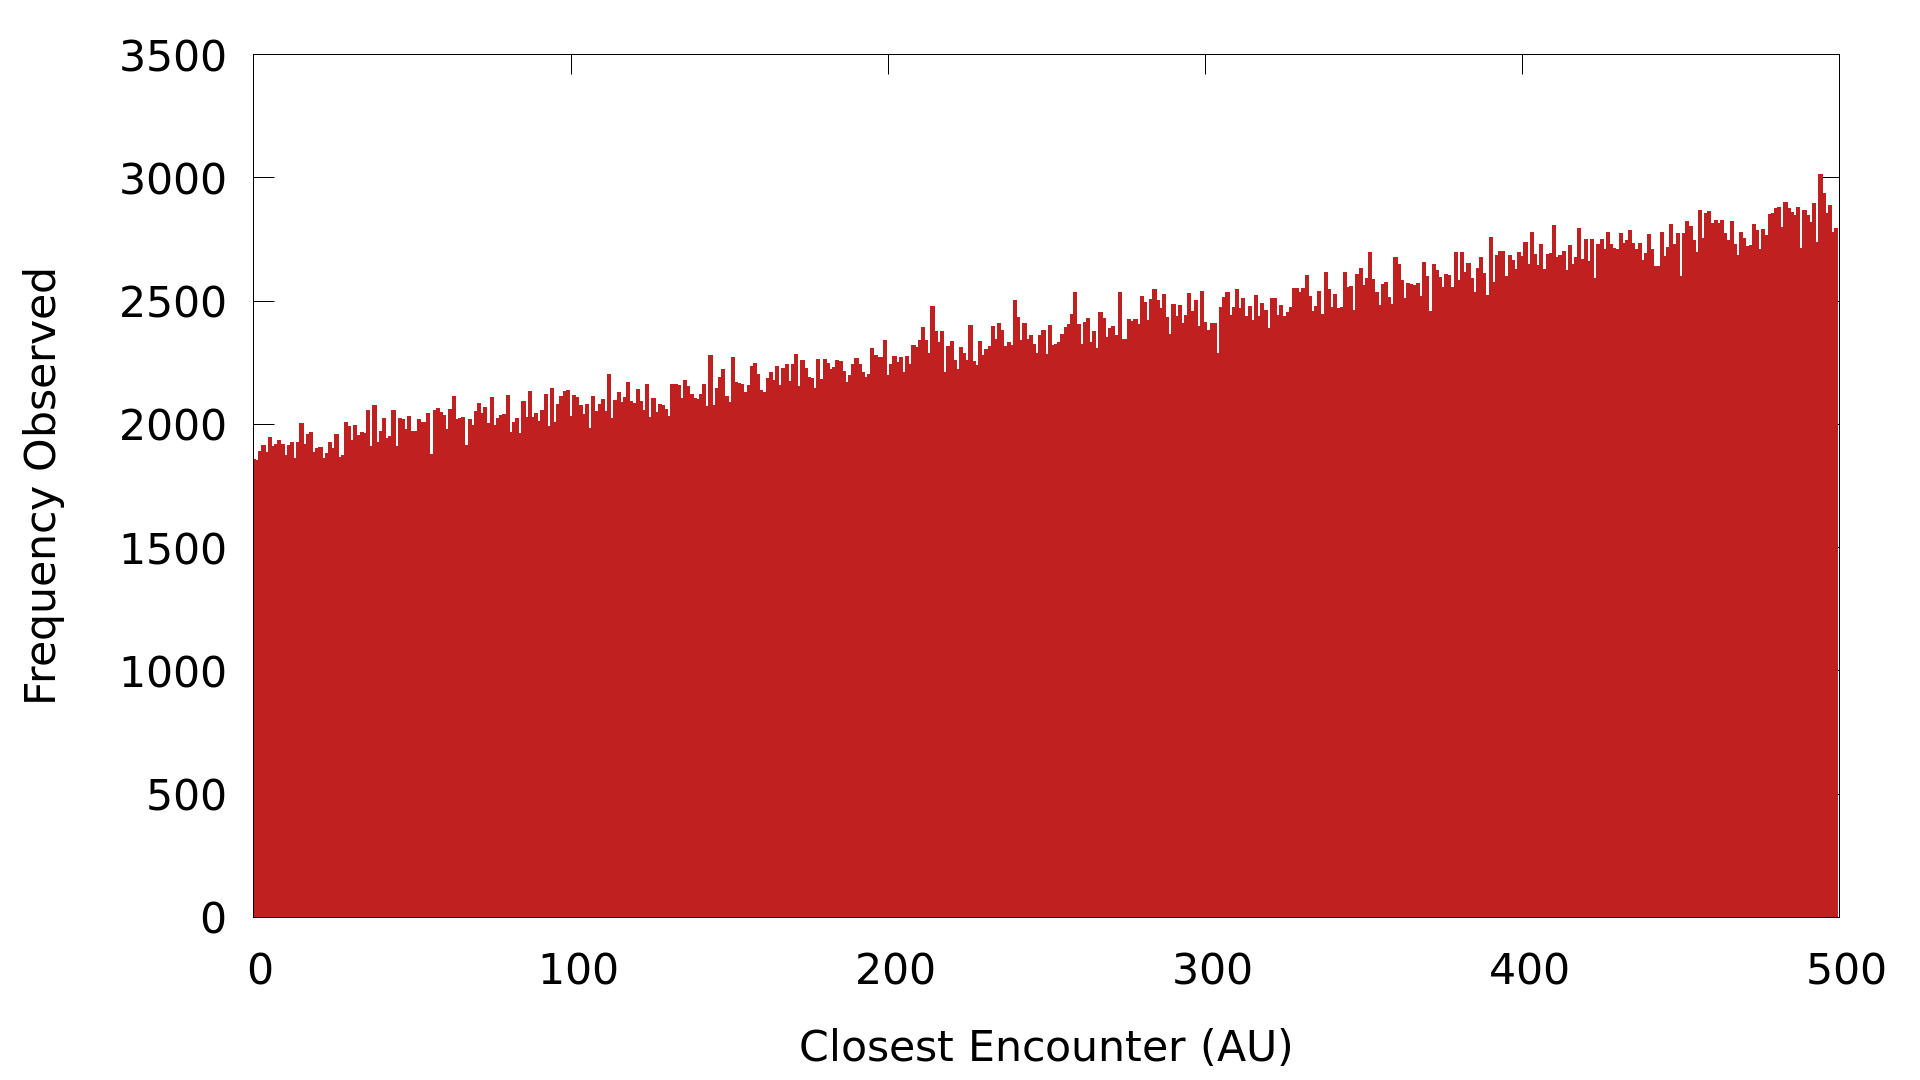
\includegraphics[width=2.25in]{encounter_distance_frequency_n1000} \\
        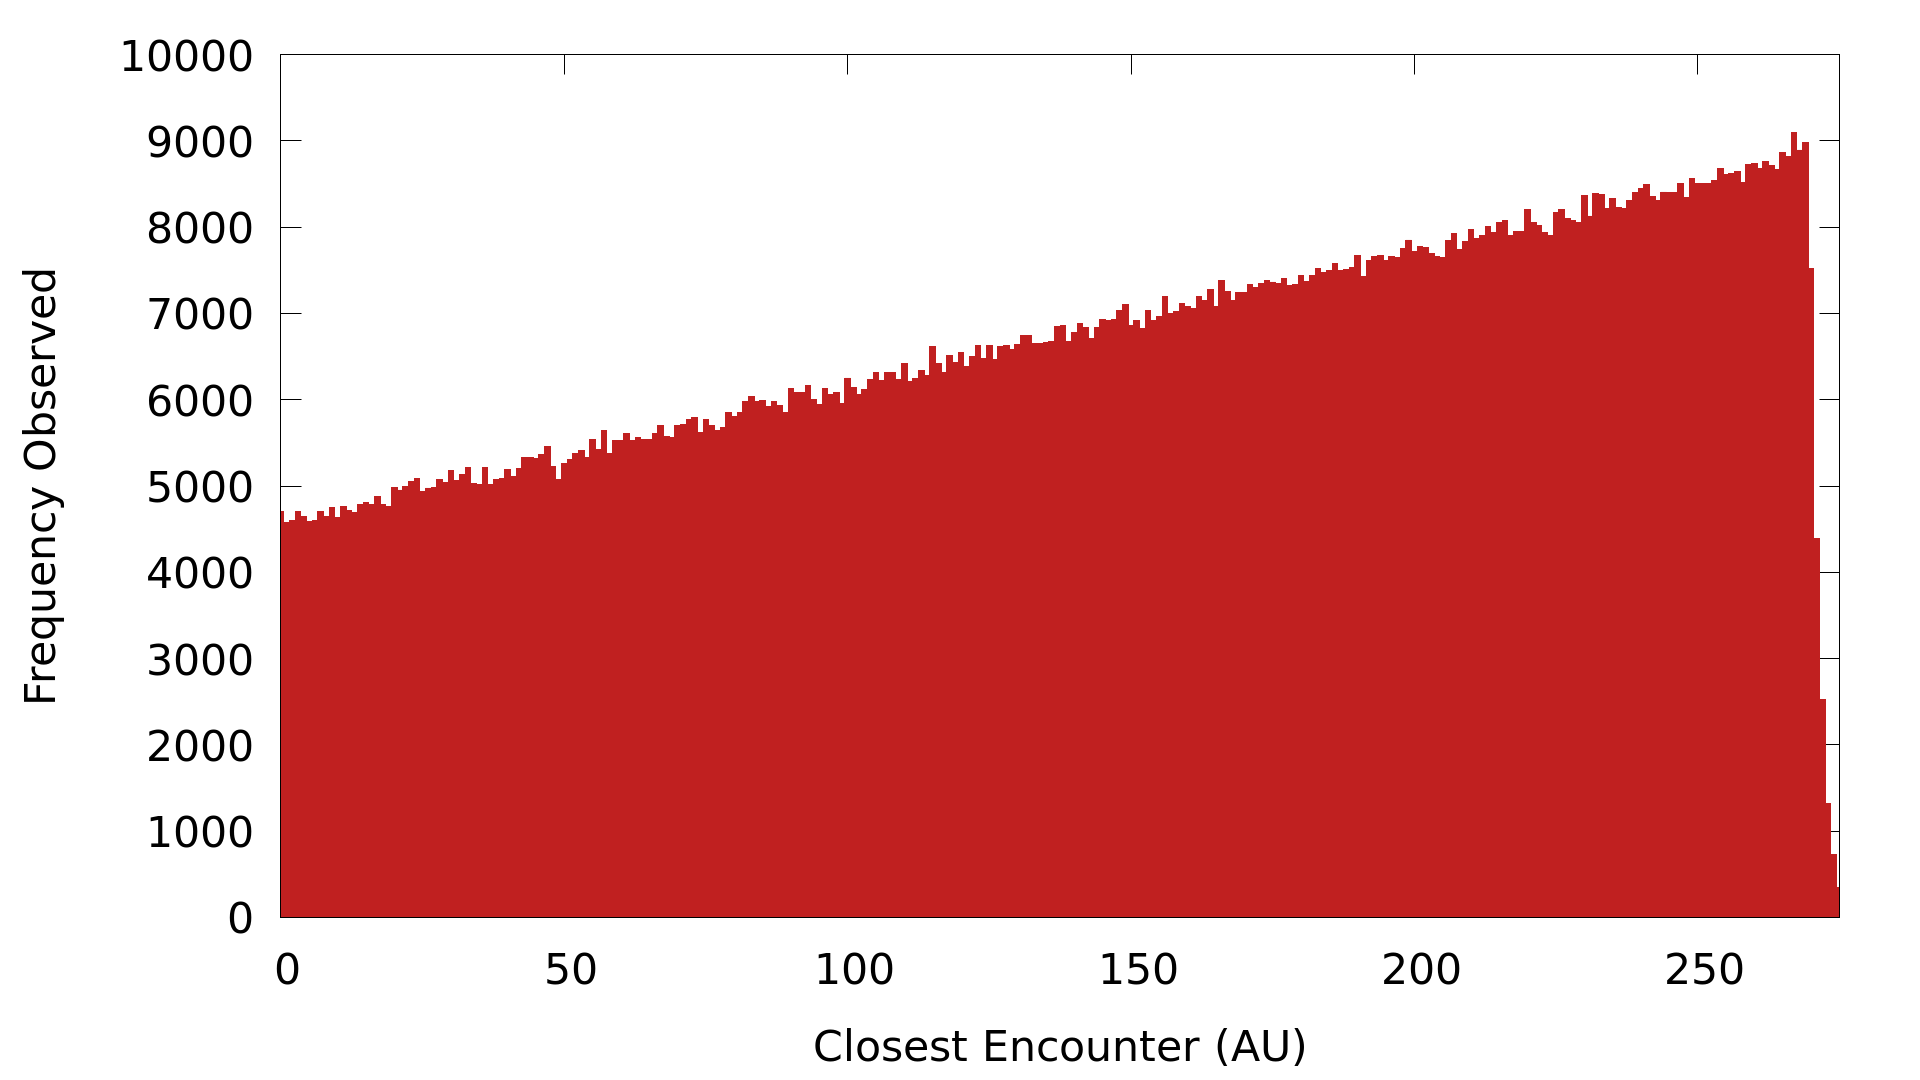
\includegraphics[width=2.25in]{encounter_distance_frequency_n4000}
    \end{figure}
\end{frame}

\begin{frame}{Phase 2: Planetary Simulations}
    \begin{itemize}
        \item Take the star encounter data and run detailed simulations.
        \item Each simulation has 2 stars and 4 planets:
            \begin{itemize}
            \item Earth, Jupiter
            \end{itemize}
        \item Stop the simulation when the stars are far apart.
    \end{itemize}
\end{frame}

\begin{frame}{Planetary Simulations}
    \begin{itemize}
        \item Initialize stars from observed encounters.
        \item Filter out distant encounters.
        \item Add desired planets.
        \item Let the simulation run until the encounter is over.
        \item Store final state of both planetary systems.
    \end{itemize}
    \begin{figure}
        \centering
        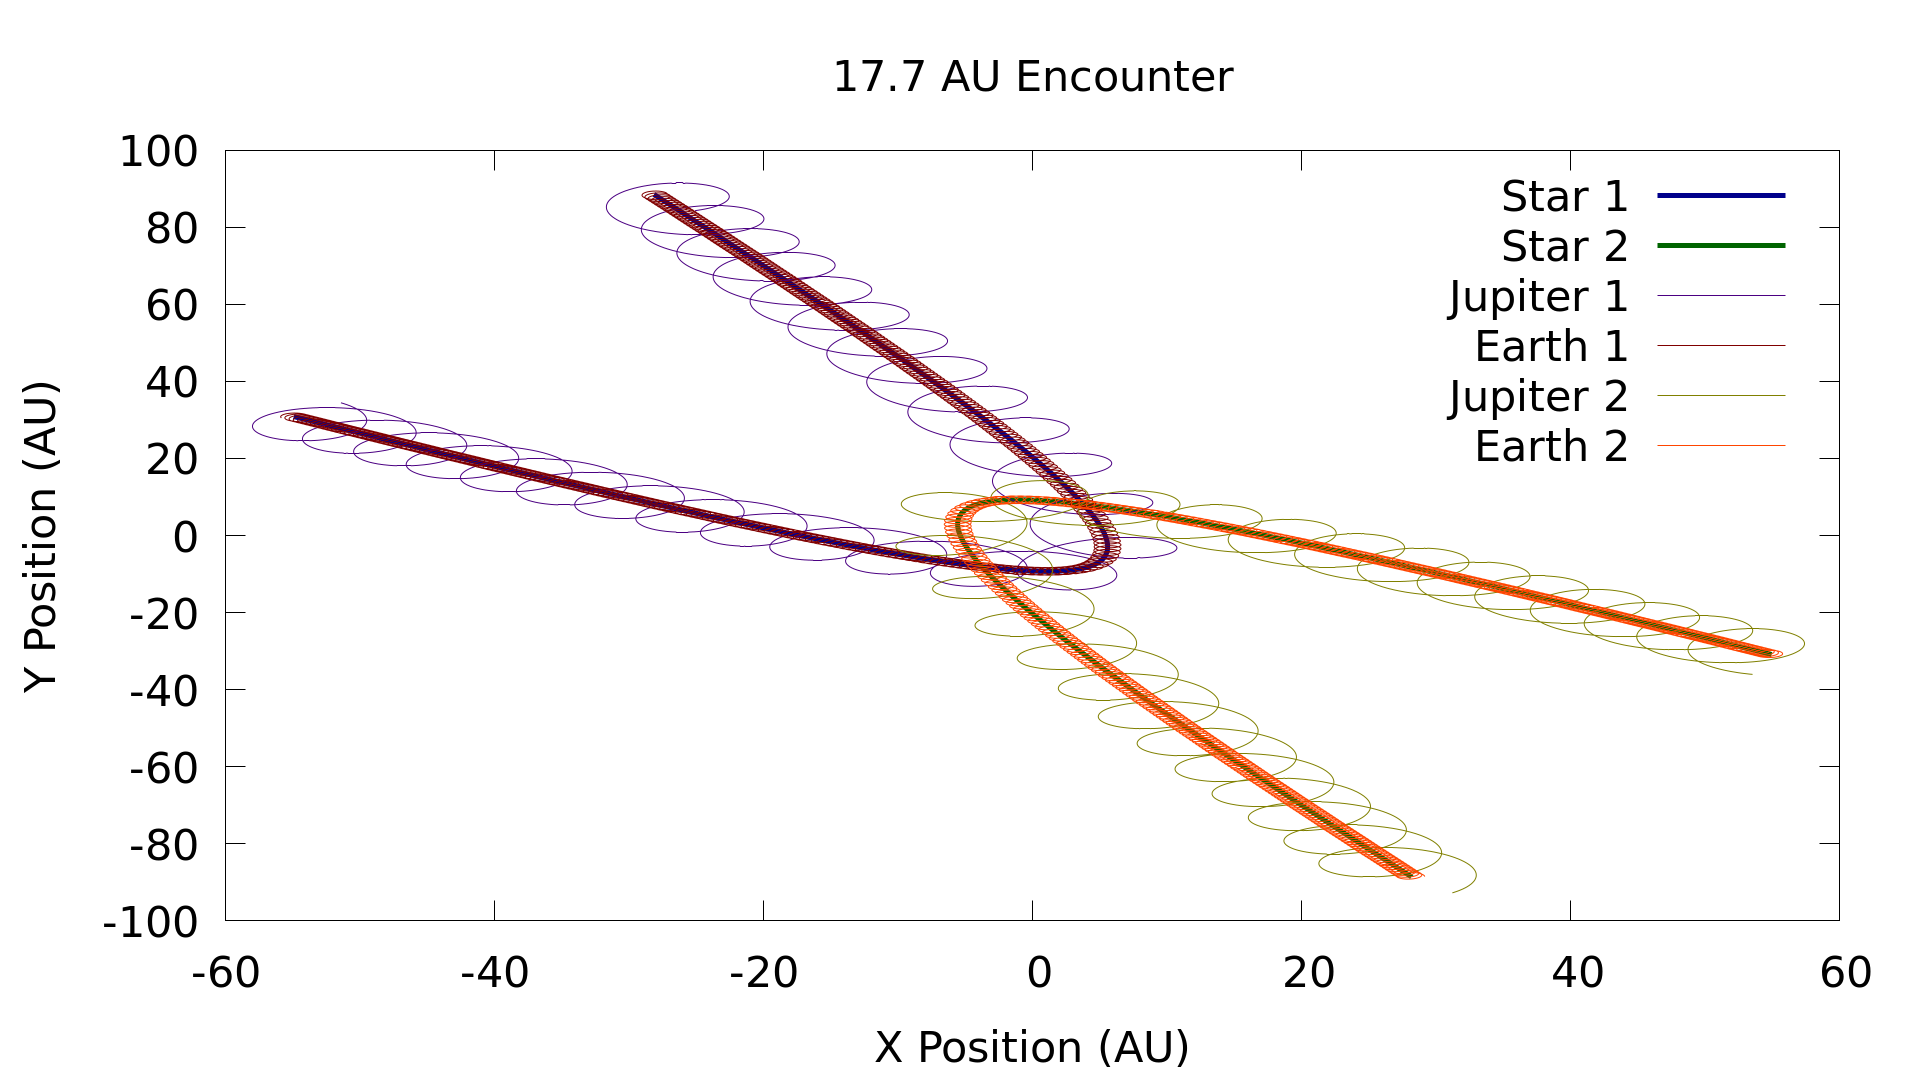
\includegraphics[height=1.75in]{17_7_AU}
    \end{figure}
\end{frame}

\begin{frame}{Simulation Example}
    \begin{figure}
        \centering
        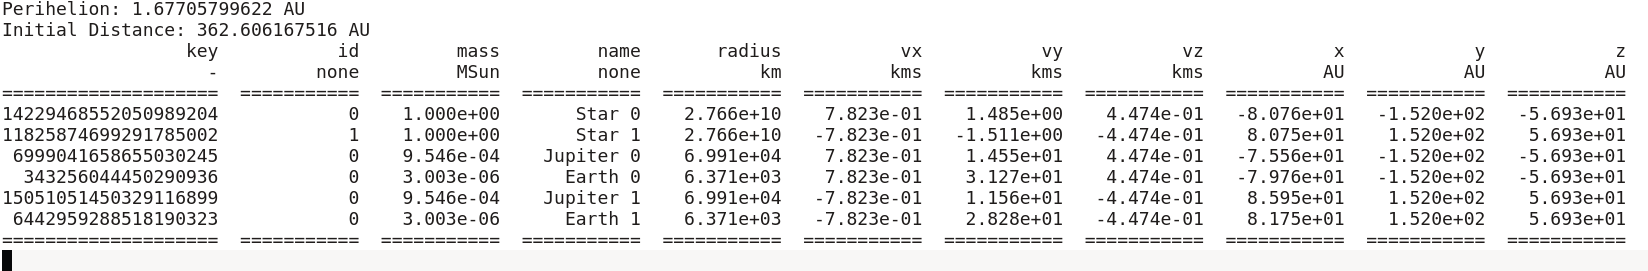
\includegraphics[width=4.00in]{Params.png}
    \end{figure}
    \begin{figure}
        \centering
        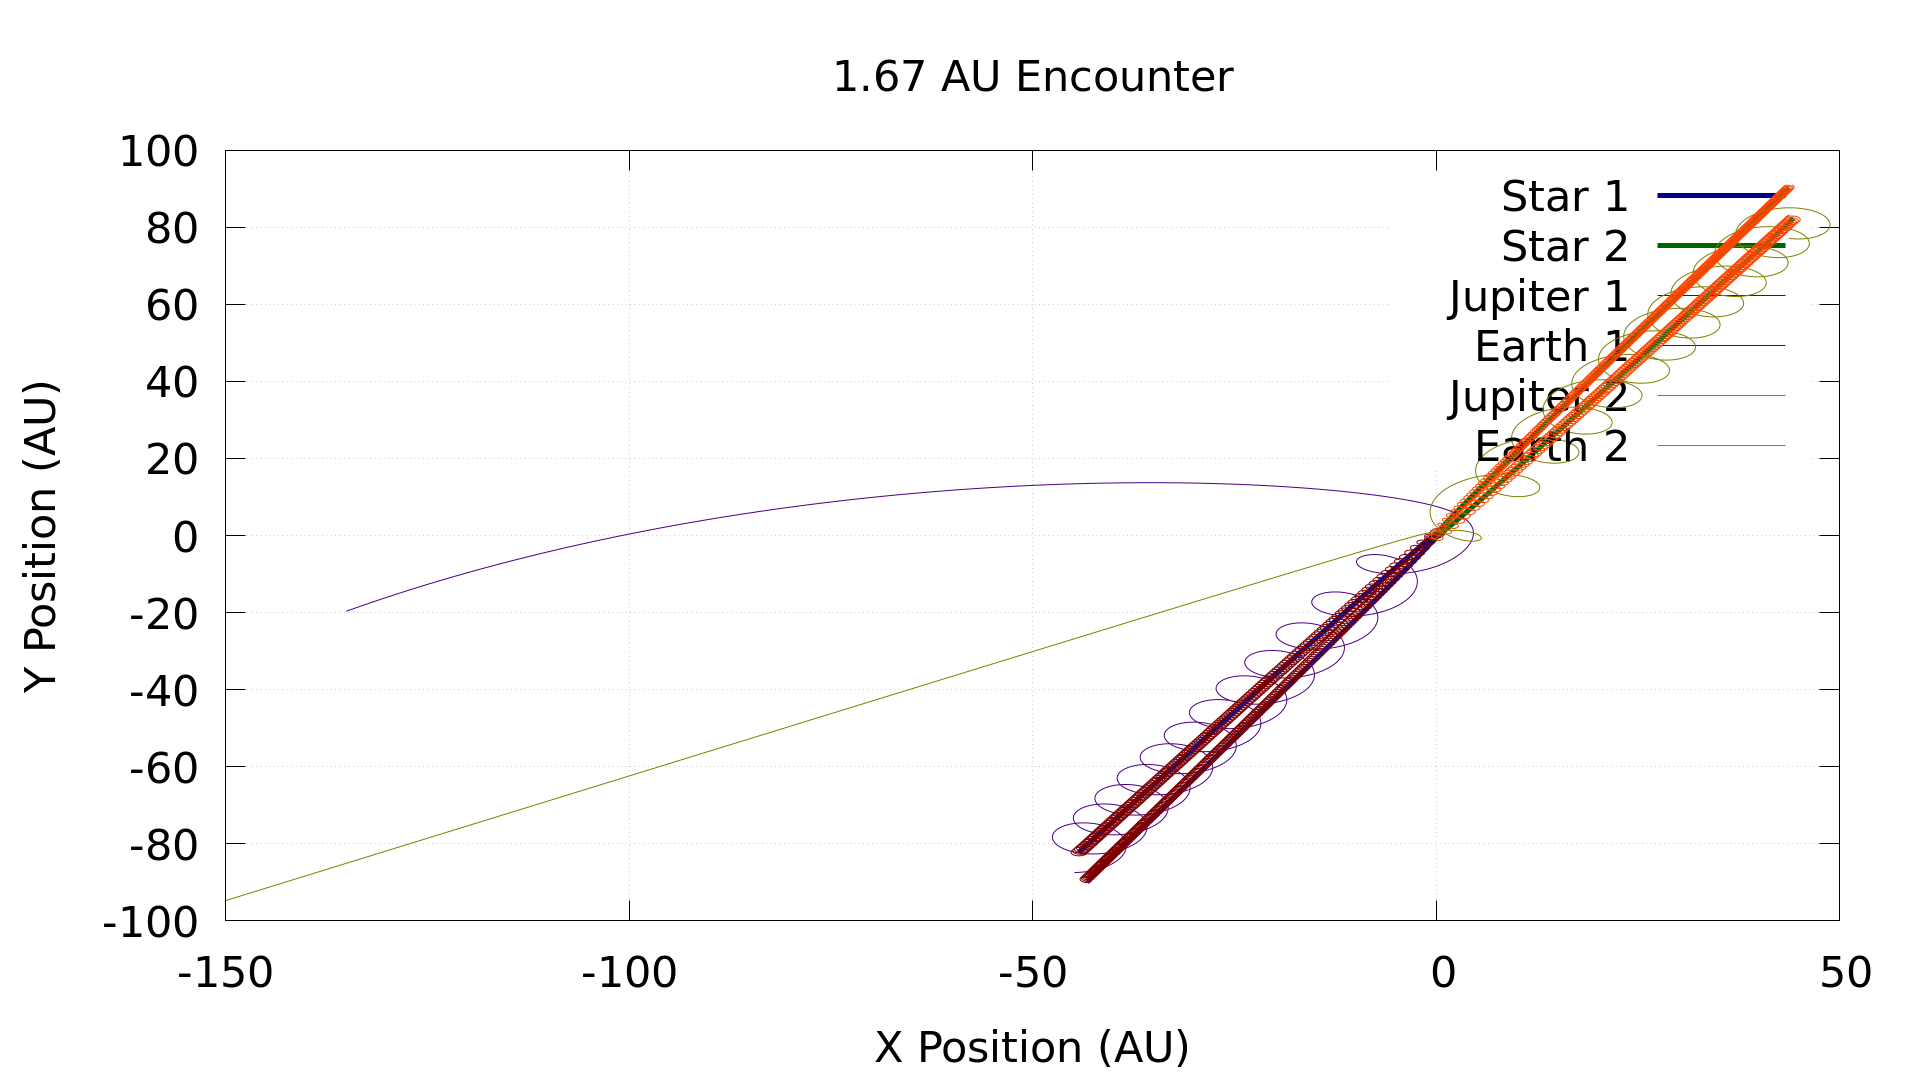
\includegraphics[height=1.75in]{ejection.png}
    \end{figure}
\end{frame}

\begin{frame}{Simulation Example}
    \begin{figure}
        \centering
        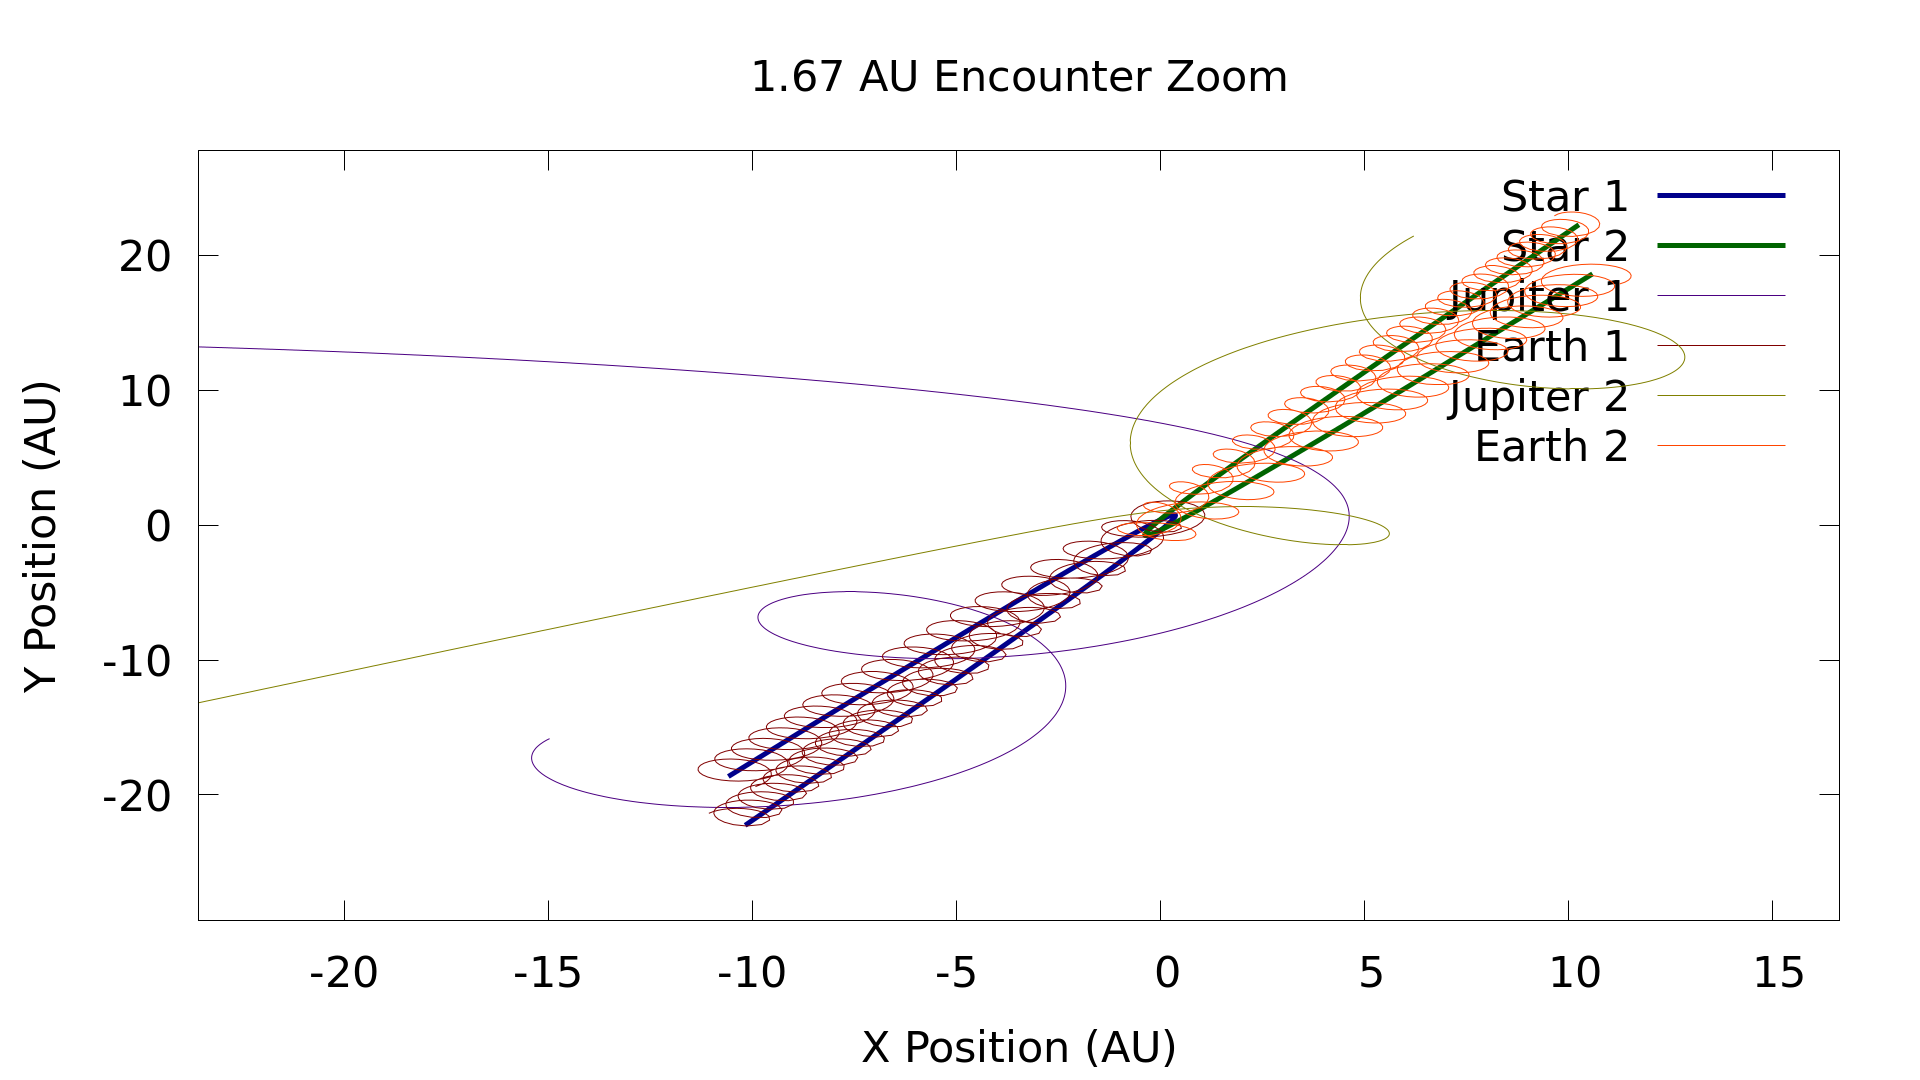
\includegraphics[width=3.75in]{1_67_AU_zoom}
    \end{figure}
\end{frame}

\begin{frame}{Simulation Example}
    \begin{figure}
        \centering
        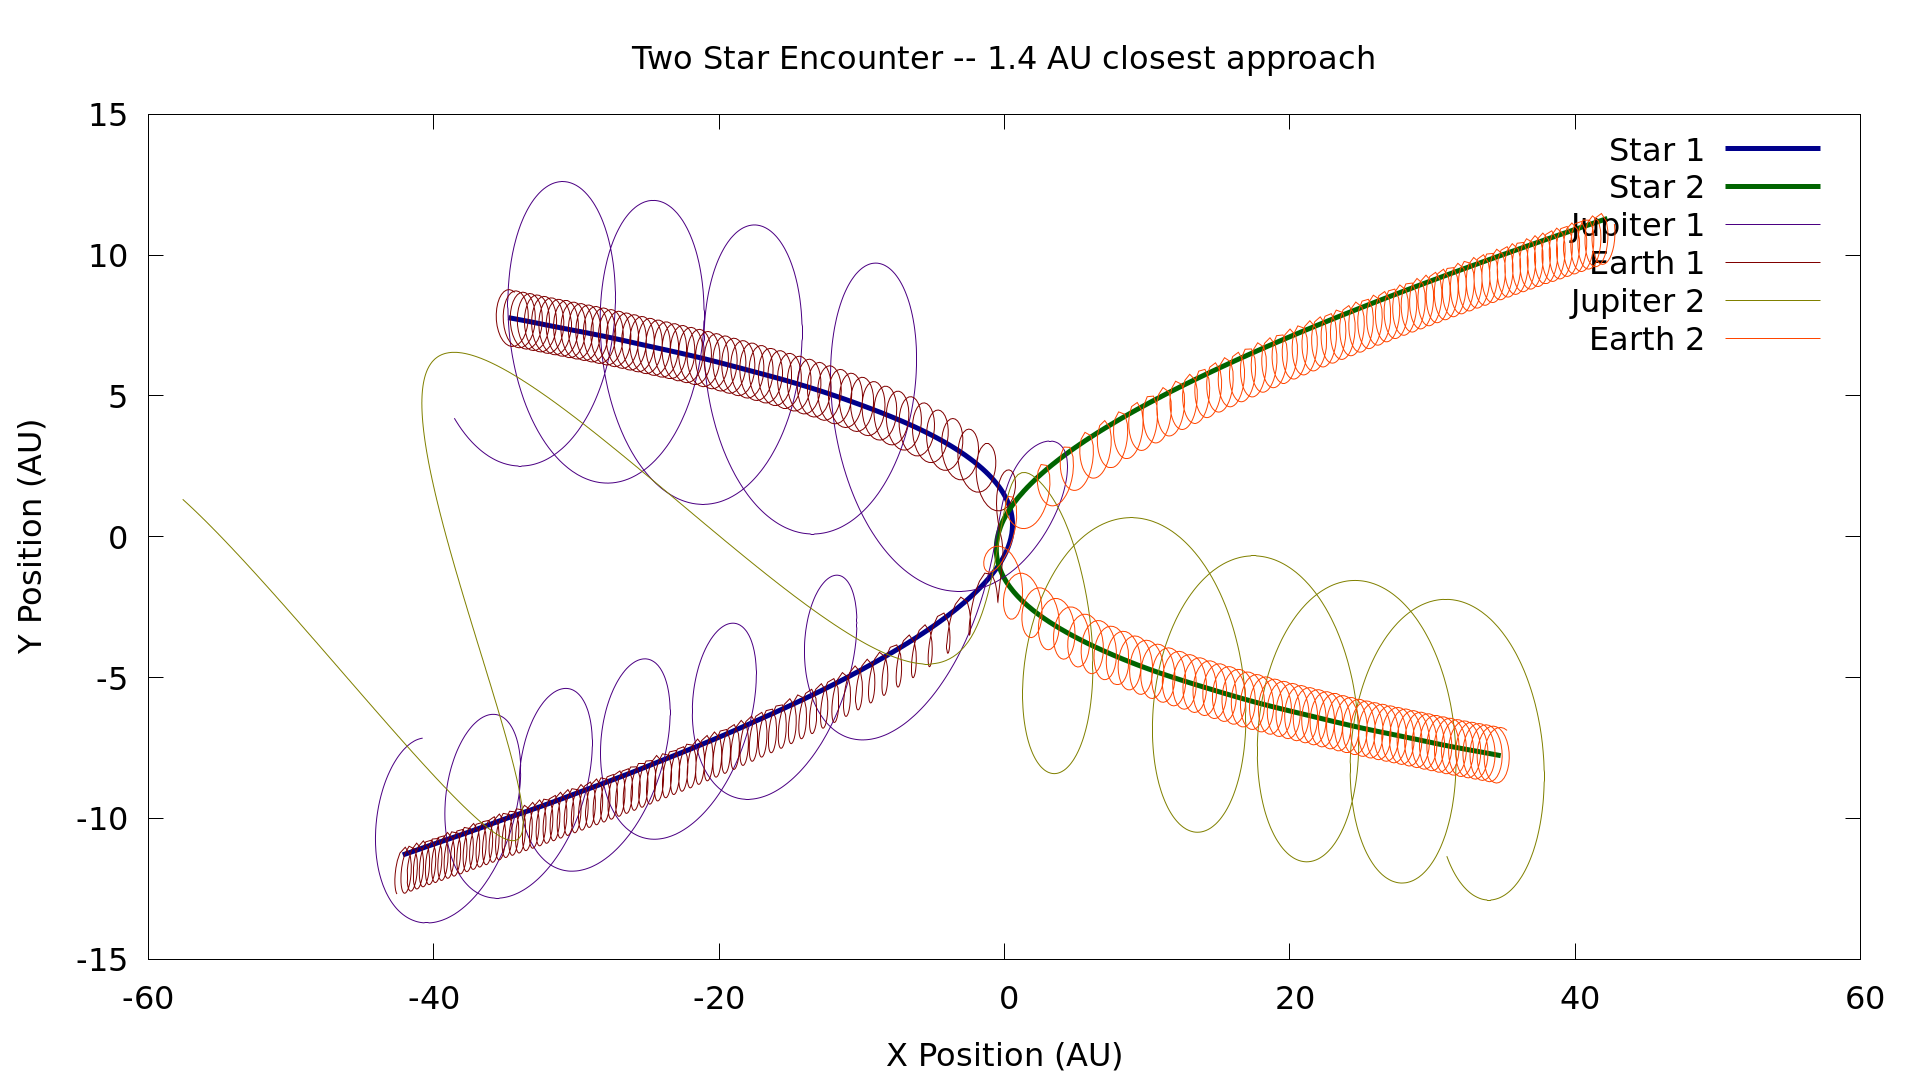
\includegraphics[height=2.5in]{1.4AU/1_4_AU_encounter_plot}
    \end{figure}
\end{frame}

\begin{frame}{Planetary Simulations}
    \begin{itemize}
        \item These simulations generate a lot of data.
            \begin{itemize}
                \item Prohibitively slow to analyze by hand.
                \item If anything needs changed, everything would have to be
                    repeated.
            \end{itemize}
        \item Develop a way to analyze data computationally.
            \begin{itemize}
                \item The orbital elements help us here.
            \end{itemize}
        \item Store the data in a way to facilitate easy computational
            analysis.
        \item Store all data needed to interpret simulations without rerunning them.
    \end{itemize}
\end{frame}

\begin{frame}{Cluster Simulation Performance}
    \begin{itemize}
        \item Need a few hundred thousand stars * Myr for each configuration.
        \item Simulating a single 4,000 star cluster for 1000 Myr requires up to 4 hours
            to run.
        \item Ran about 200 of these clusters to get enough encounters.
        \item A naive approach would require around 800 hours to complete just the 4,000
            star clusters!
    \end{itemize}
\end{frame}

\begin{frame}{Planet Simulation Performance}
    \begin{itemize}
        \item Require about 30 seconds each.
        \item Far more numerous -- 55,000 total simulations.
        \item In series, this would require approximately 400 hours.
    \end{itemize}
\end{frame}

\begin{frame}{Parallelism}
    \begin{columns}
    \column{0.60\textwidth}
        \begin{itemize}
            \item Each simulation is independent of all others.
            \item Each node of Draco has many processing "cores".
            \item Running many simulations in parallel can reduce
                time required dramatically.
        \end{itemize}
    \column{0.40\textwidth}
        \begin{figure}
            \centering
            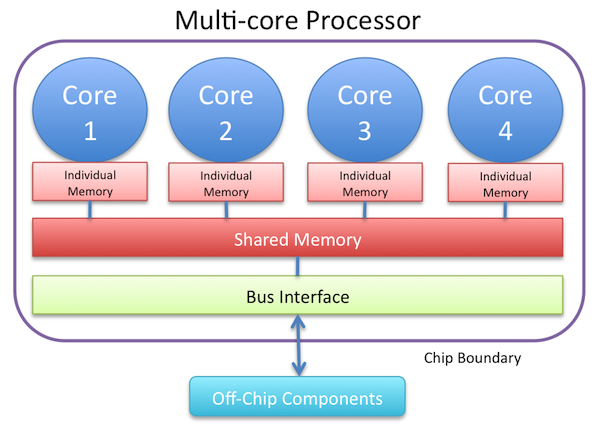
\includegraphics[width=2.0in]{multicore}
        \end{figure}
    \end{columns}
\end{frame}

\begin{frame}{Parallelism Results}
    \begin{itemize}
        \item Cluster Simulations
            \begin{itemize}
                \item 3-6 per node.
                \item Run over 6 nodes.
                \item About 25 simultaneous simulations.
                \item Time reduced to $\approxeq$ 3 days for largest clusters.
            \end{itemize}
        \item Planetary Simulations
            \begin{itemize}
                \item 8 per node.
                \item Run over 6 nodes.
                \item About 50 simultaneous simulations.
                \item Time reduced to $\approxeq$ 24 hours.
            \end{itemize}
    \end{itemize}
\end{frame}

% Database stuff ?

\begin{frame}{Analysis}
    \begin{itemize}
        \item We want to analyze the results of many
            simulations.
        \item Using numerical categorization such the orbital elements,
            we can try to answer questions about the simulation results.
        \item Develop analyses that can be used on any data set.
    \end{itemize}
\end{frame}

\section{Results}

\begin{frame}{Results: Eccentricity, Jupiter}
    \begin{itemize}
        \item All planets are initialized to have zero eccentricity.
        \item Higher eccentricities correlate to larger changes.
        \item Eccentricities $\ge 1.0$ imply a planet escaped from its
            original system.
            \begin{itemize}
                \item These aren't included on the plot.
            \end{itemize}
    \end{itemize}
    \begin{figure}
        \centering
        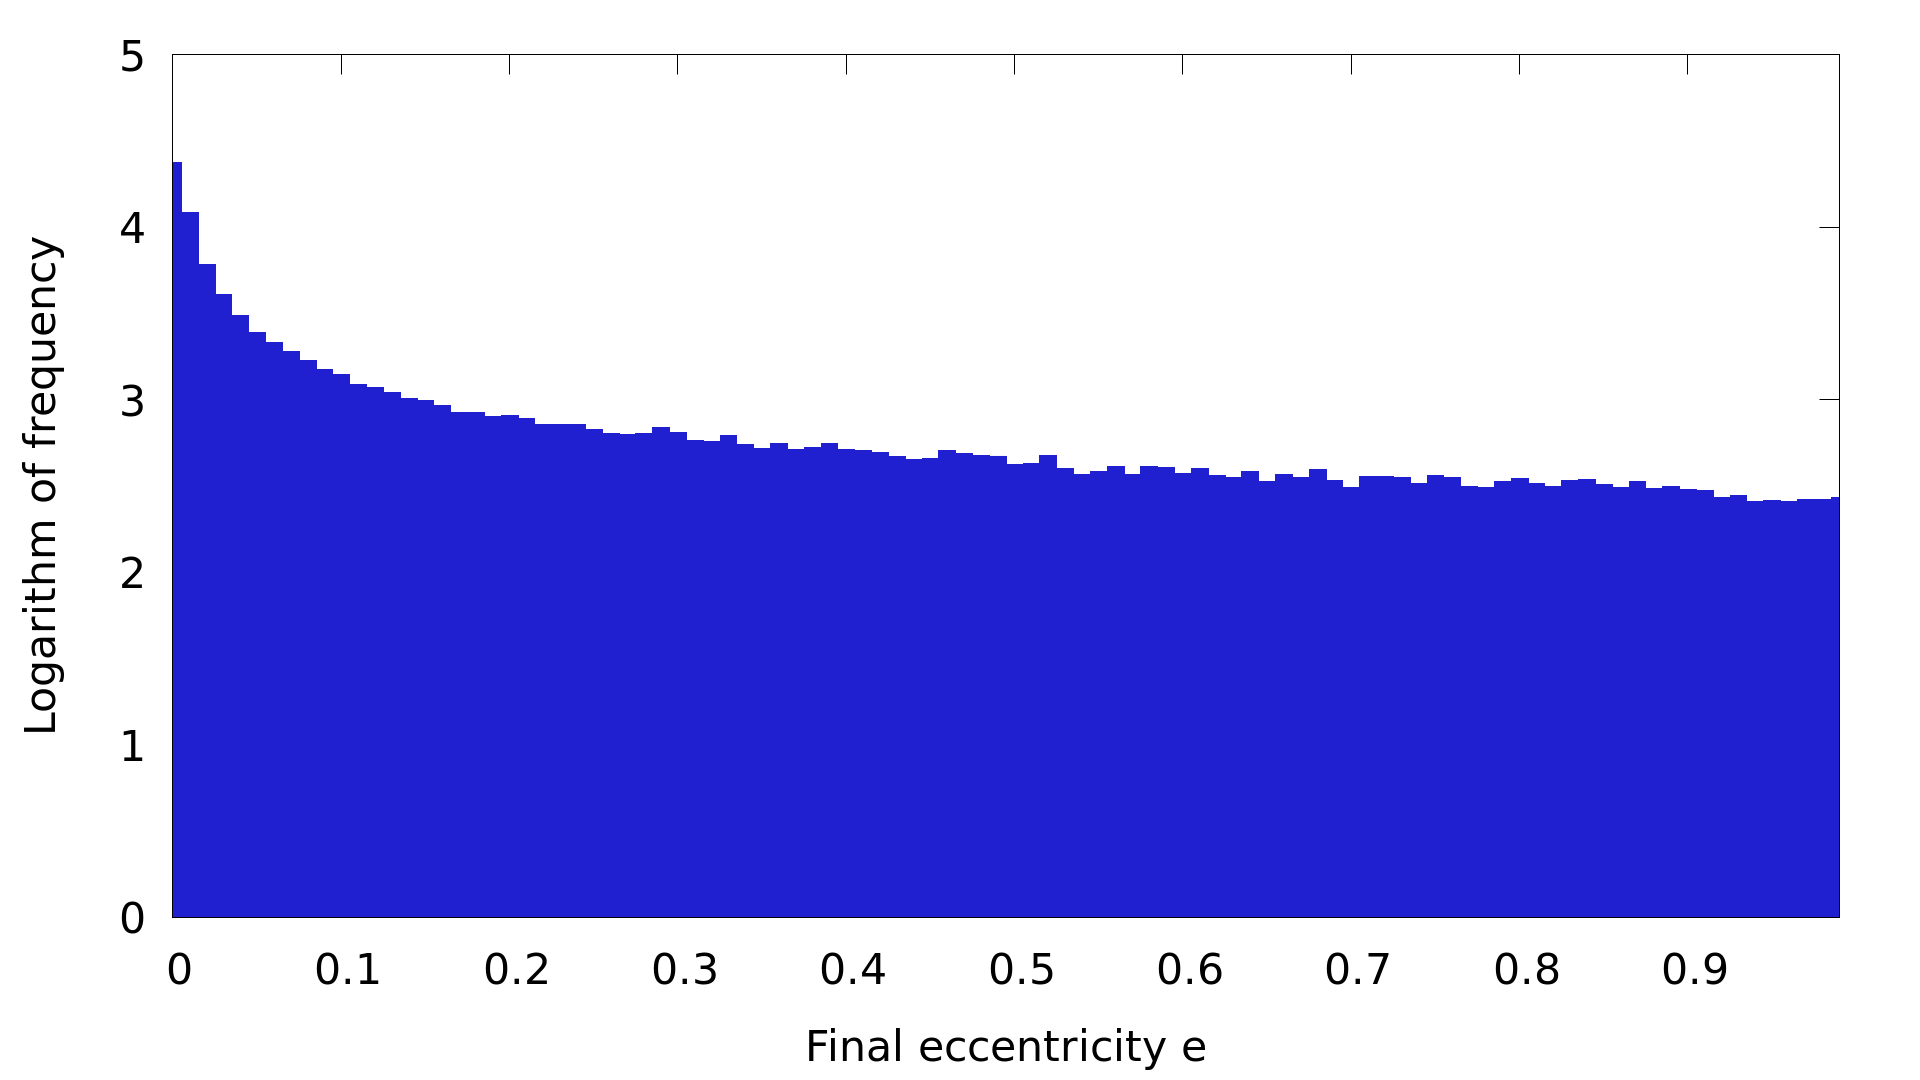
\includegraphics[height=1.75in]{eccentricity_jupiter_1000.png}
    \end{figure}
\end{frame}

\begin{frame}{Results: Eccentricity, Earth}
    \begin{figure}
        \centering
        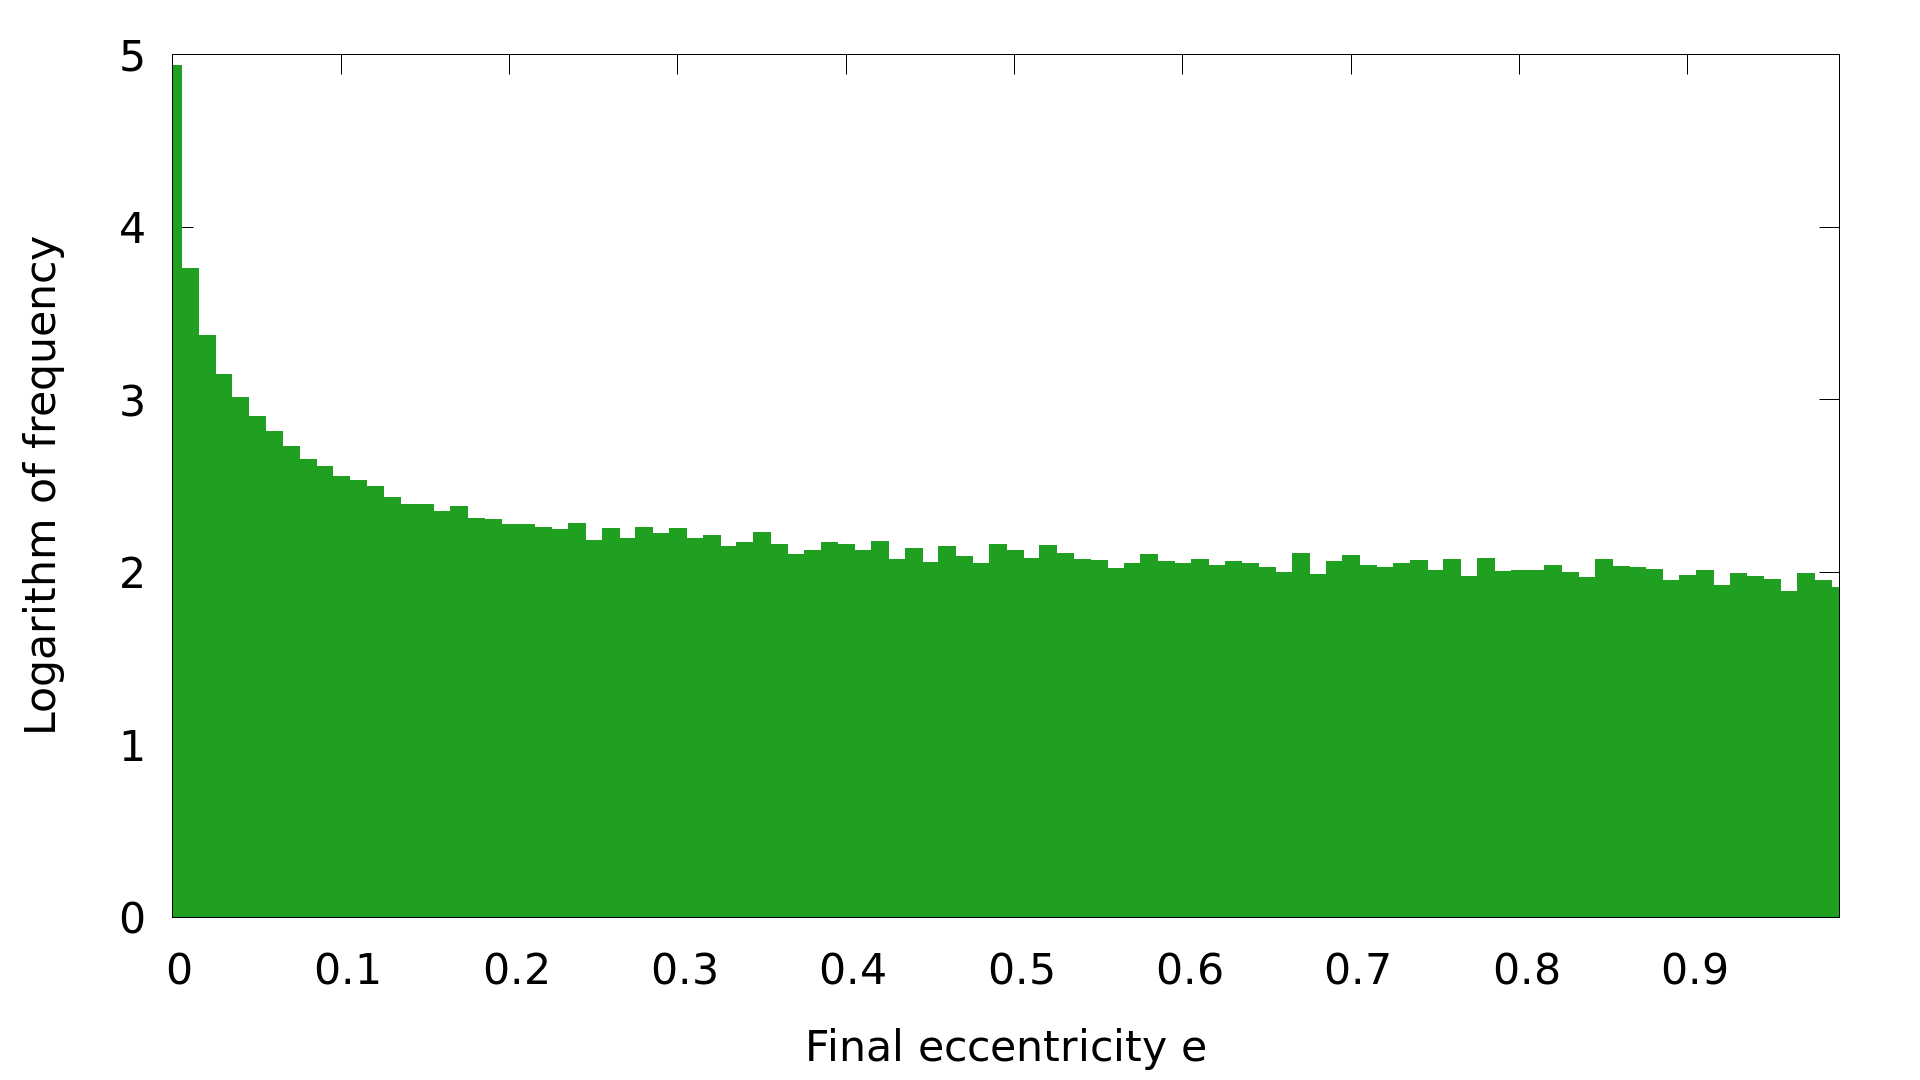
\includegraphics[height=1.75in]{eccentricity_earth_1000.png}
    \end{figure}
    \begin{itemize}
        \item Most planets are relatively unaffected by the encounter.
        \item As eccentricity gets more extreme, frequency decreases.
        \item Some planets are thrown into highly eccentric orbits.
        \item Jupiters are much more affected than Earths.
    \end{itemize}
\end{frame}

\begin{frame}{Results: Eccentricity}
    \begin{columns}
    \column{0.33\textwidth}
        \begin{itemize}
            \item Cluster size does not significantly affect eccentricity distribution
        \end{itemize}
    \column{0.66\textwidth}
        \begin{figure}
            \caption{Jupiter eccentricity spectrum for 1000, 2000 and 4000 star clusters.}
            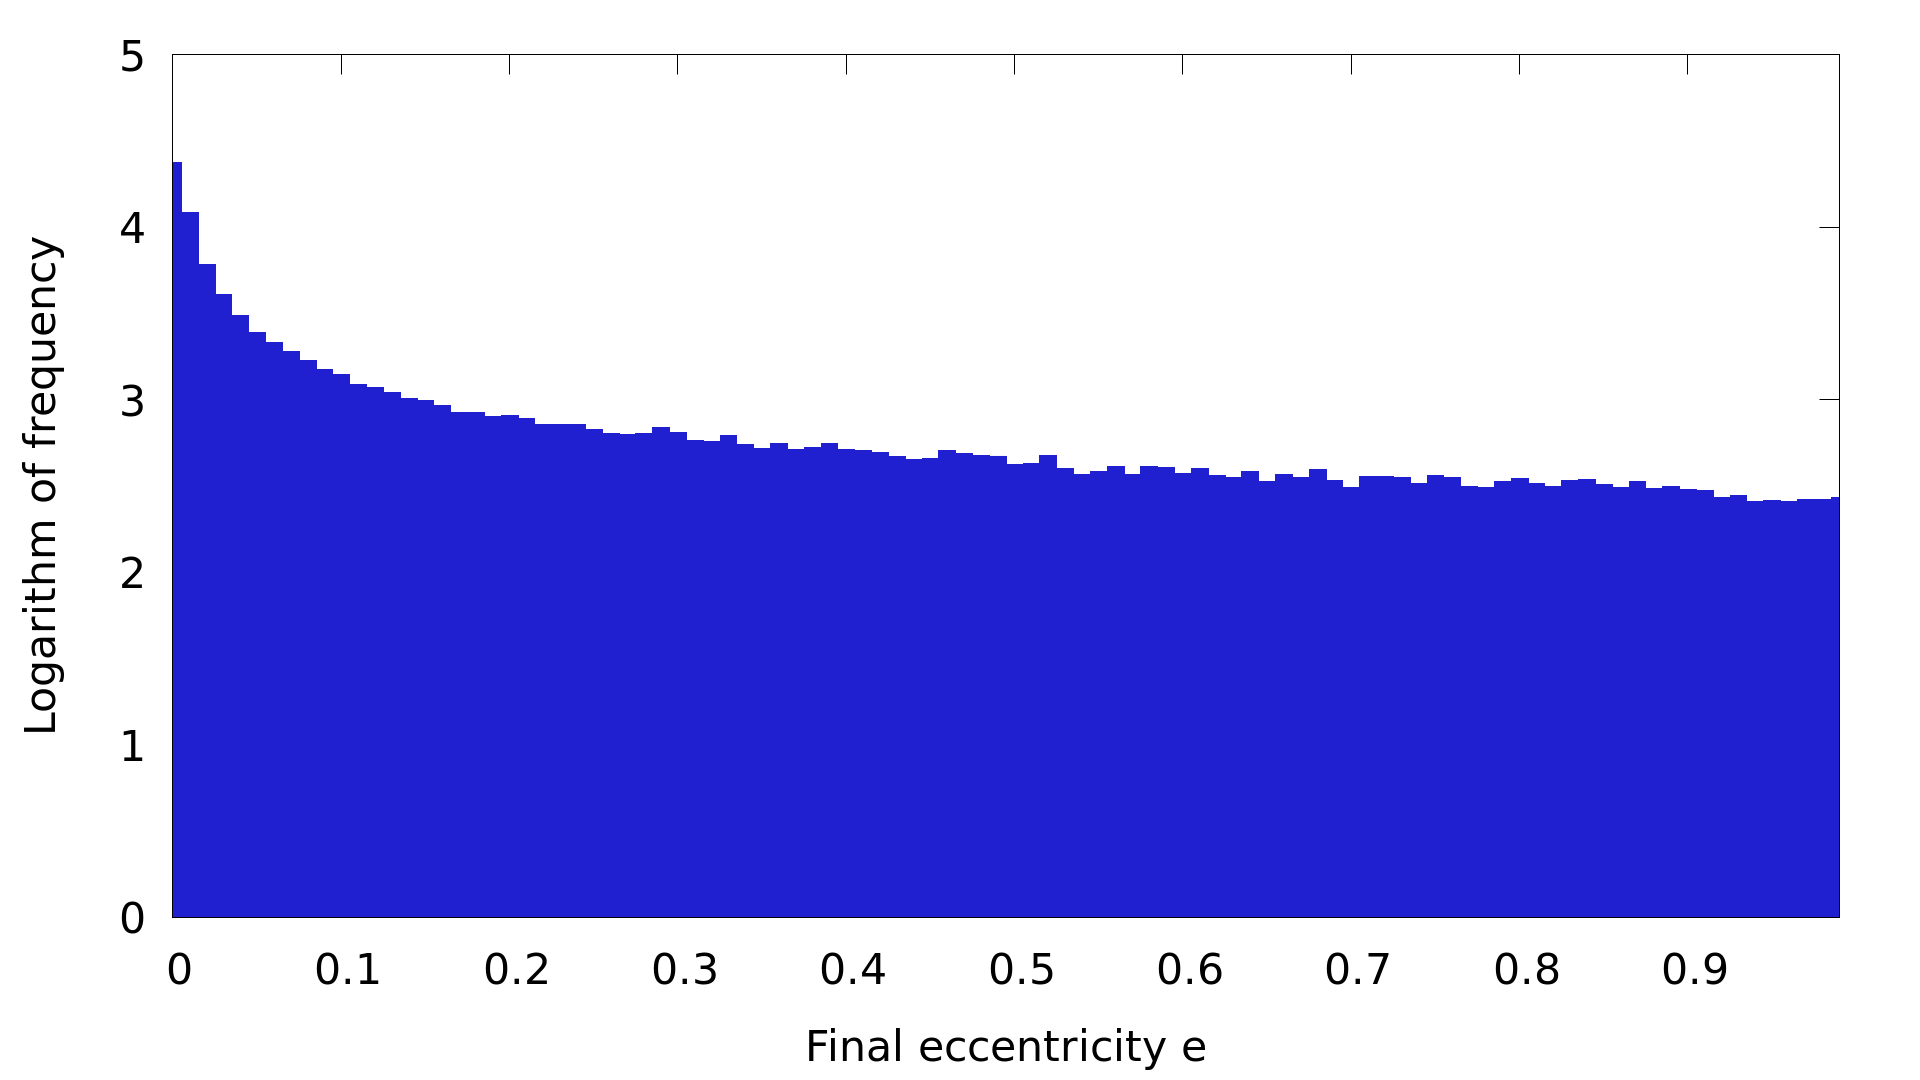
\includegraphics[height=0.90in]{eccentricity_jupiter_1000.png} \\
            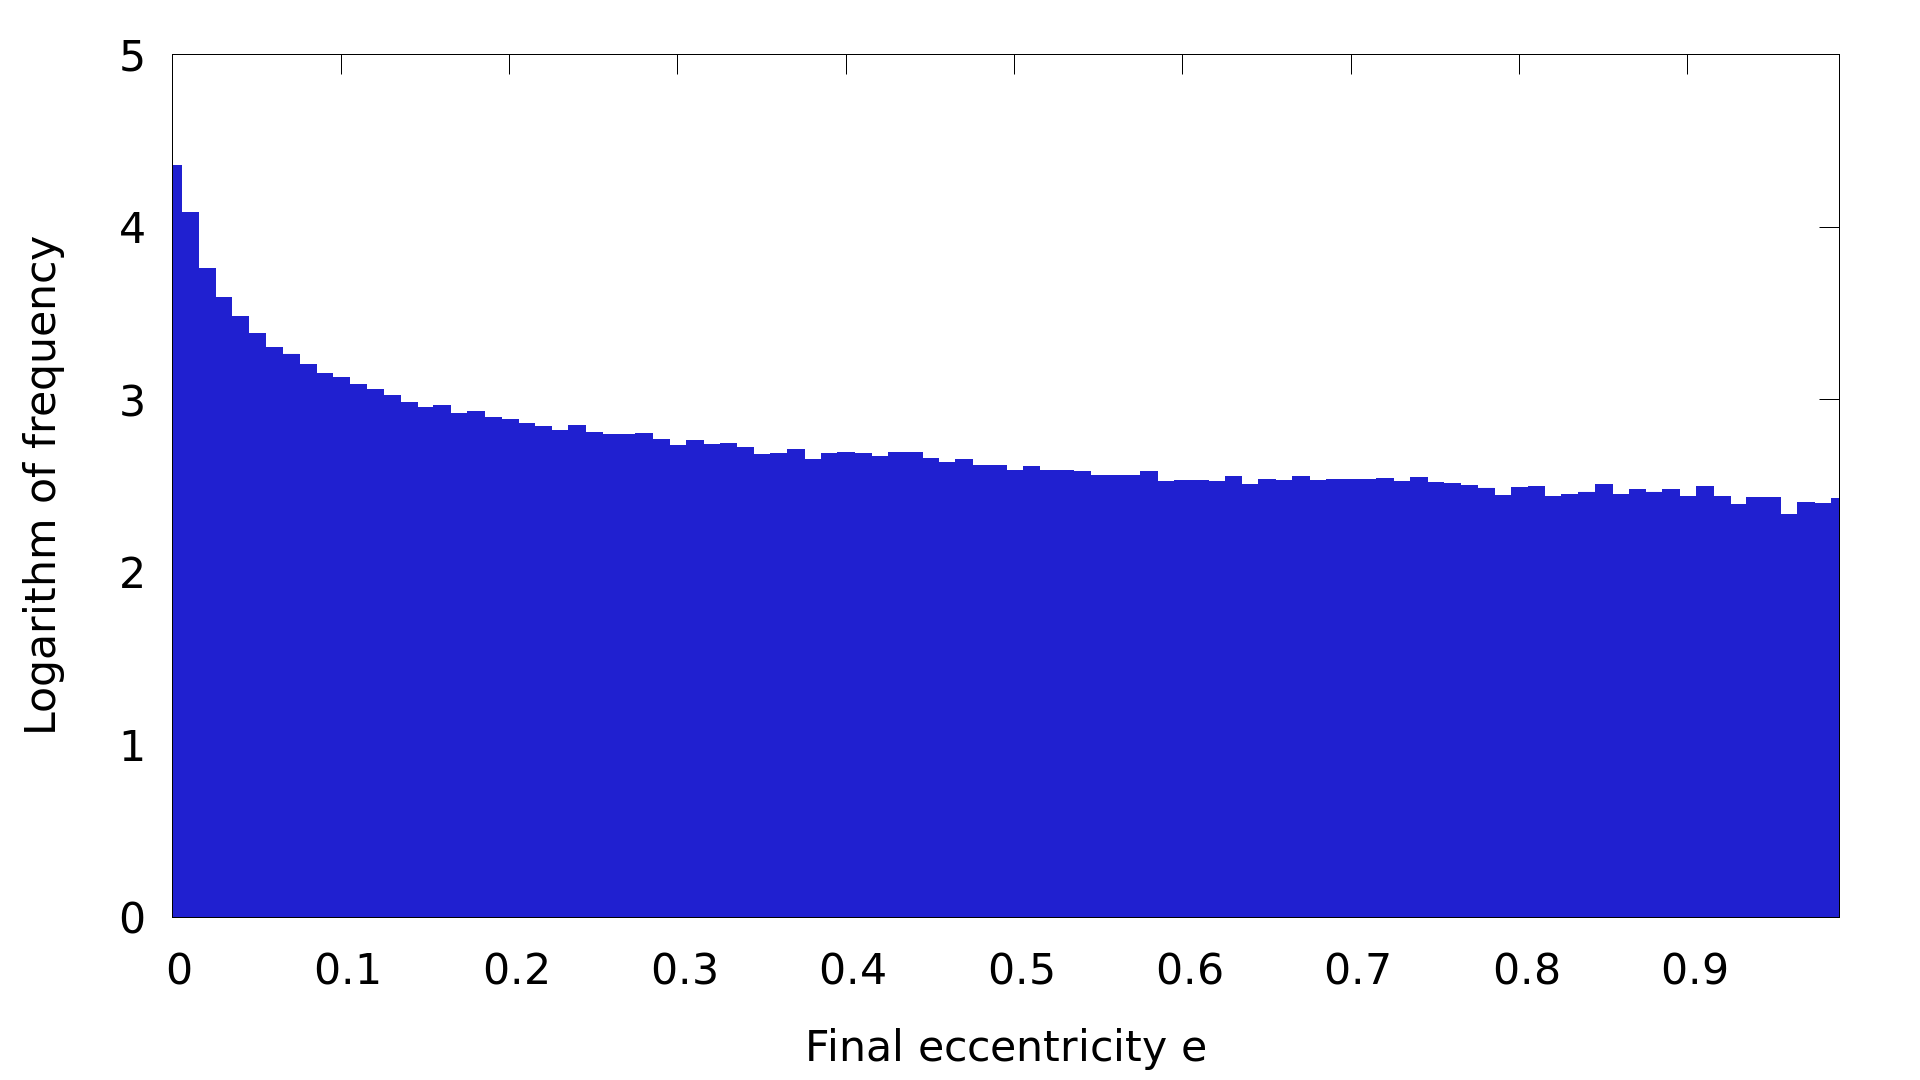
\includegraphics[height=0.90in]{eccentricity_jupiter_2000.png} \\
            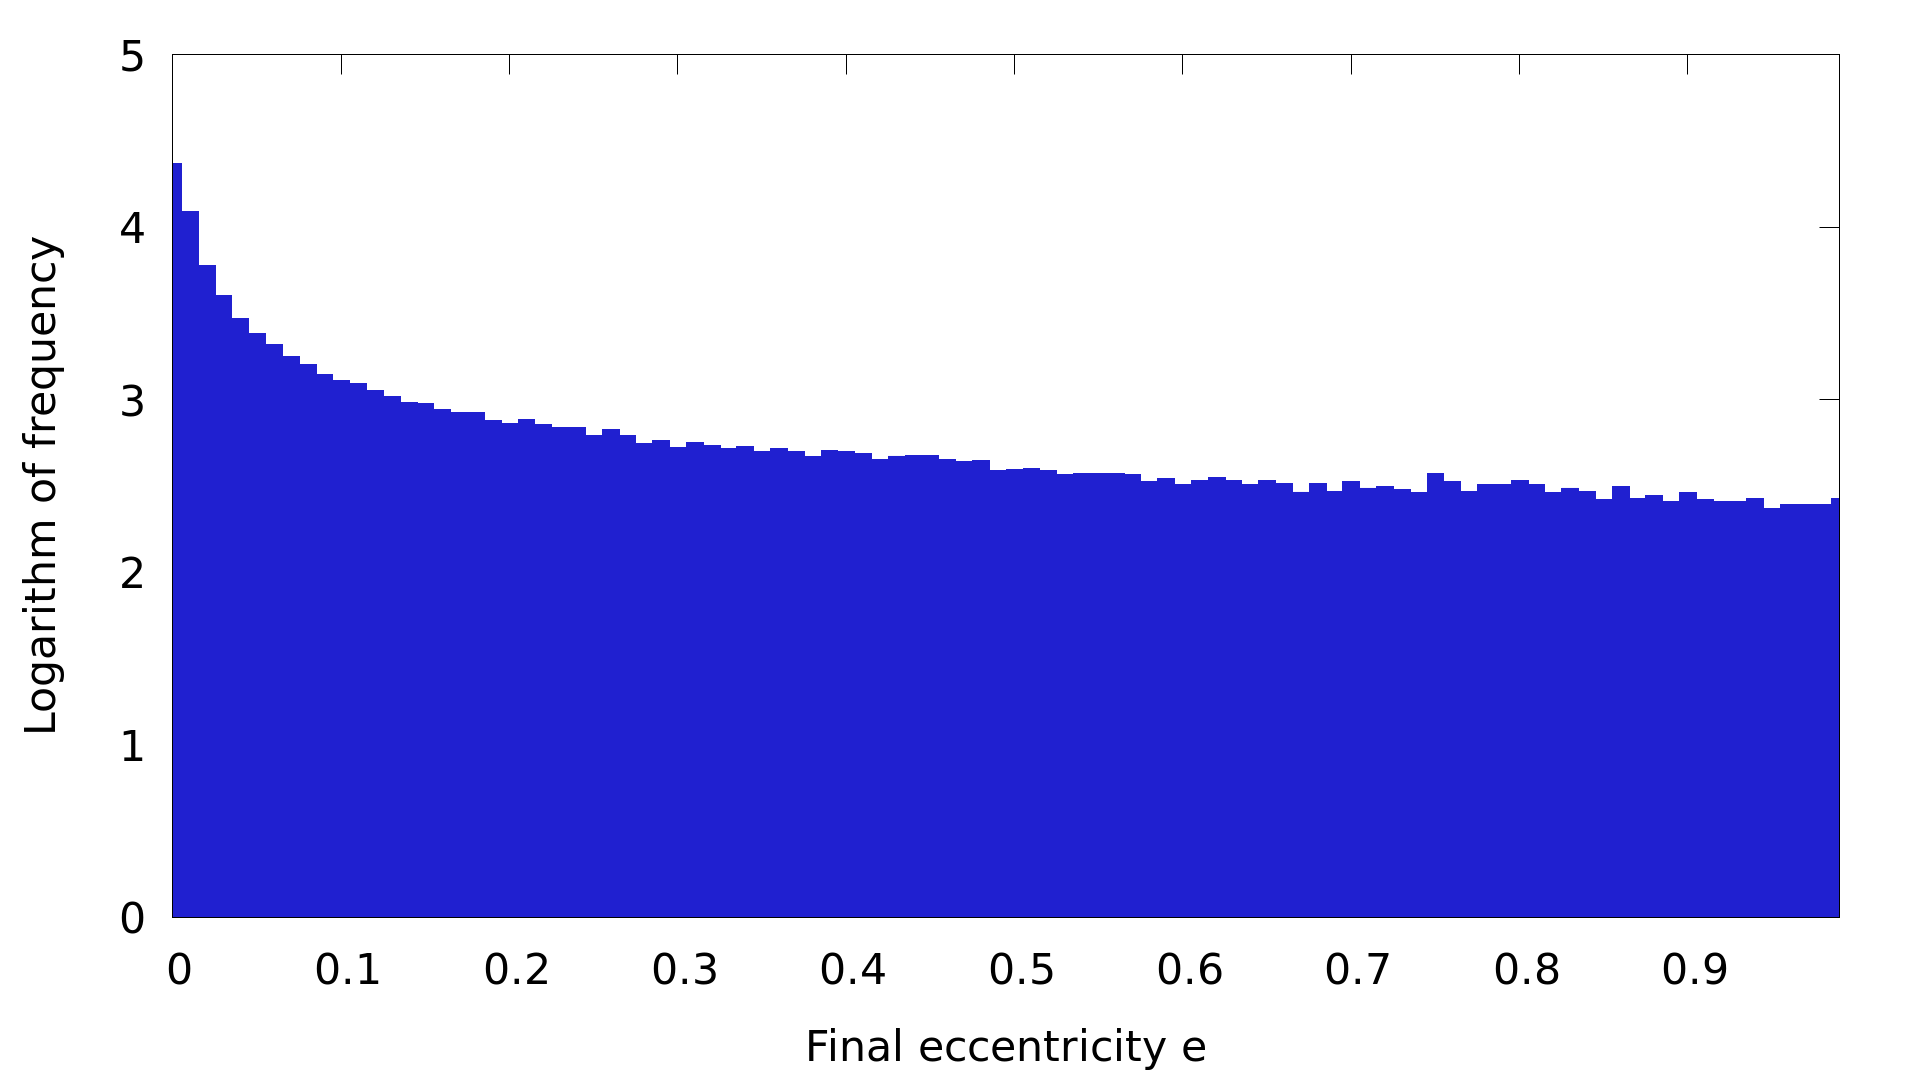
\includegraphics[height=0.90in]{eccentricity_jupiter_4000.png}
        \end{figure}
    \end{columns}
\end{frame}

\begin{frame}{Planet Ejection and Capture}
    \begin{table}[H]
        \centering
        \tiny
        \caption{Final states of Jupiter planets.}
        \begin{tabular}{|llll|}
            \hline
            \textbf{Cluster Size} & \textbf{Remaining Planets} & \textbf{Ejected Planets} & \textbf{Captured Planets} \\
            \hline
            1000 & 46,935 & 6,472 & 1,593 \\
            2000 & 46,925 & 6,528 & 1,548 \\
            4000 & 47,146 & 6,343 & 1,511 \\
            \hline
        \end{tabular}
    \end{table}
    \begin{table}[H]
        \centering
        \tiny
        \caption{Final states of Earth planets.}
        \begin{tabular}{|llll|}
            \hline
            \textbf{Cluster Size} & \textbf{Remaining Planets} & \textbf{Ejected Planets} & \textbf{Captured Planets} \\
            \hline
            1000 & 53,427 & 1,245 & 328 \\
            2000 & 53,489 & 1,229 & 282 \\
            4000 & 53,413 & 1,299 & 288 \\
            \hline
        \end{tabular}
    \end{table}
\end{frame}

\begin{frame}{Results: Periastron}
    \begin{itemize}
        \item Jupiter gets close to its star $\approxeq 3$ times more frequently than Earth.
    \end{itemize}
    \begin{tabular}{cc}
        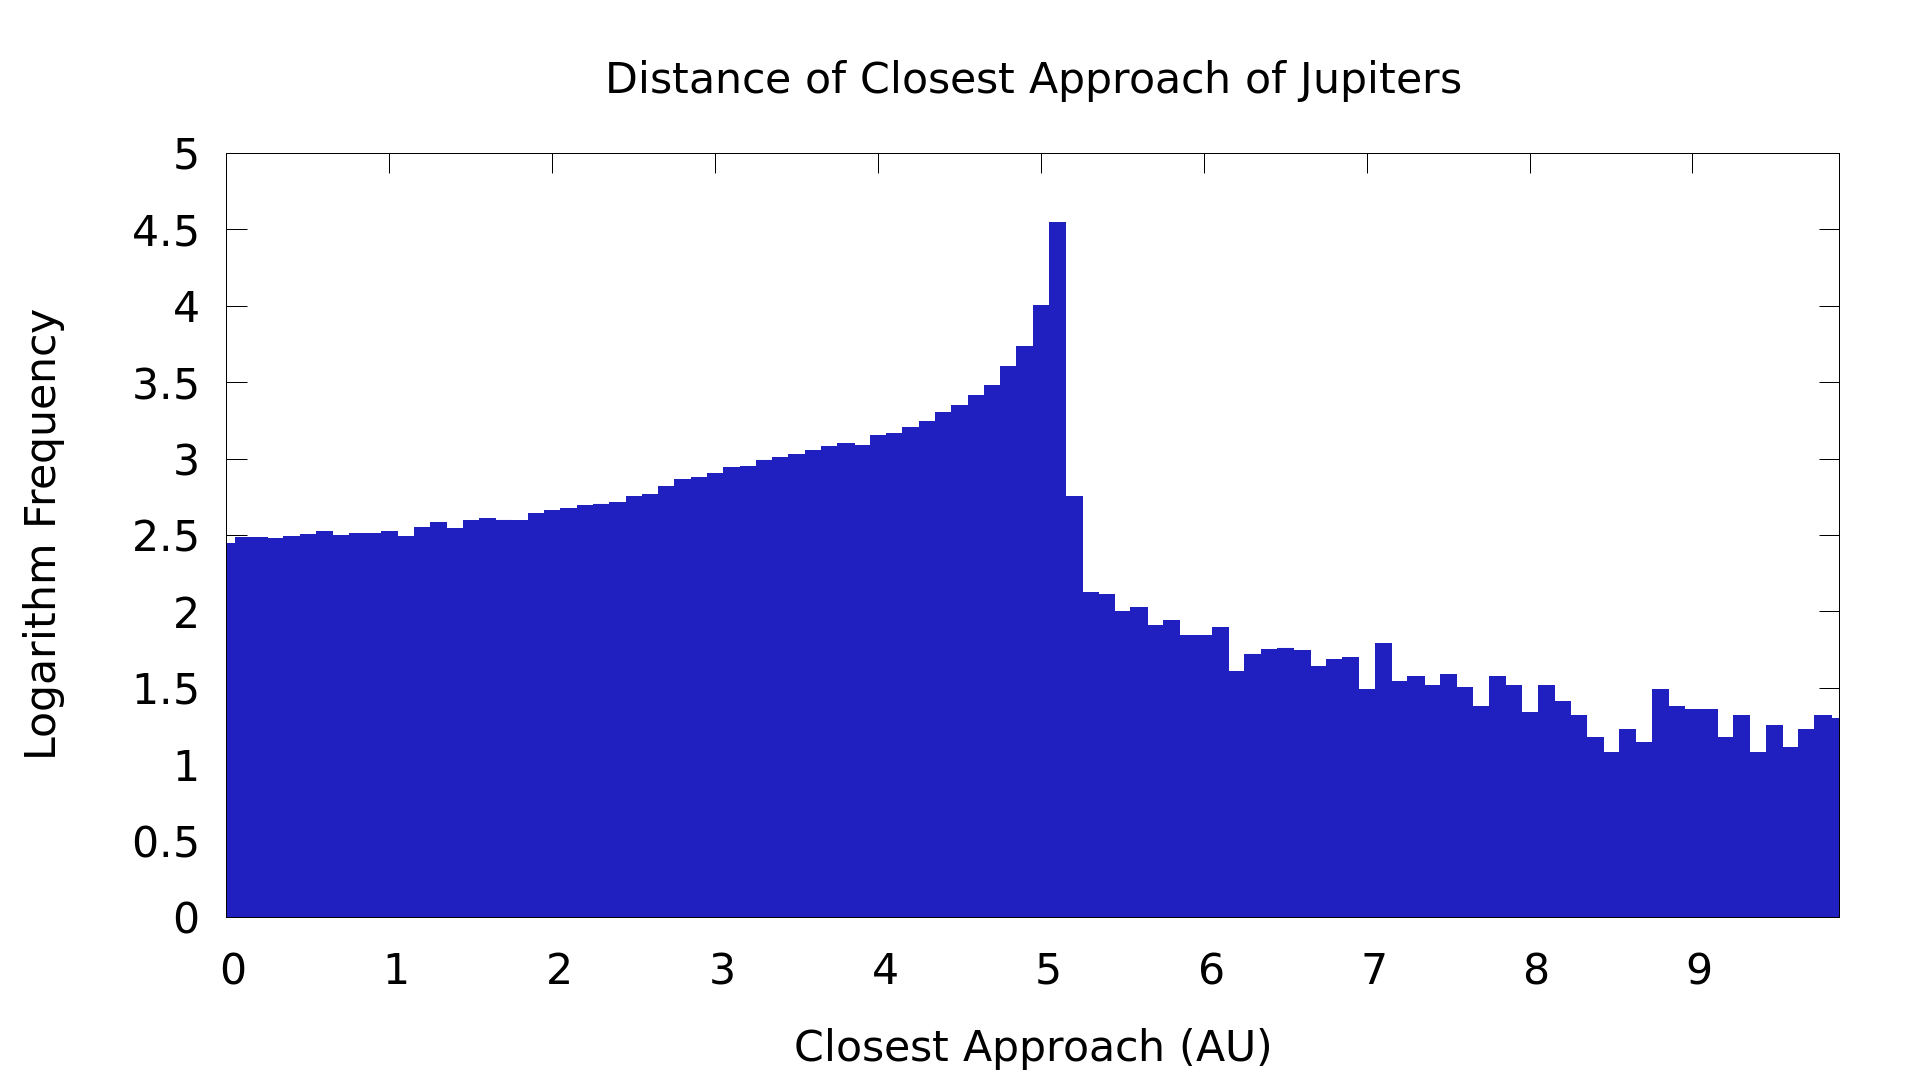
\includegraphics[height=1.20in]{periastron_jupiter_1000.png} &
        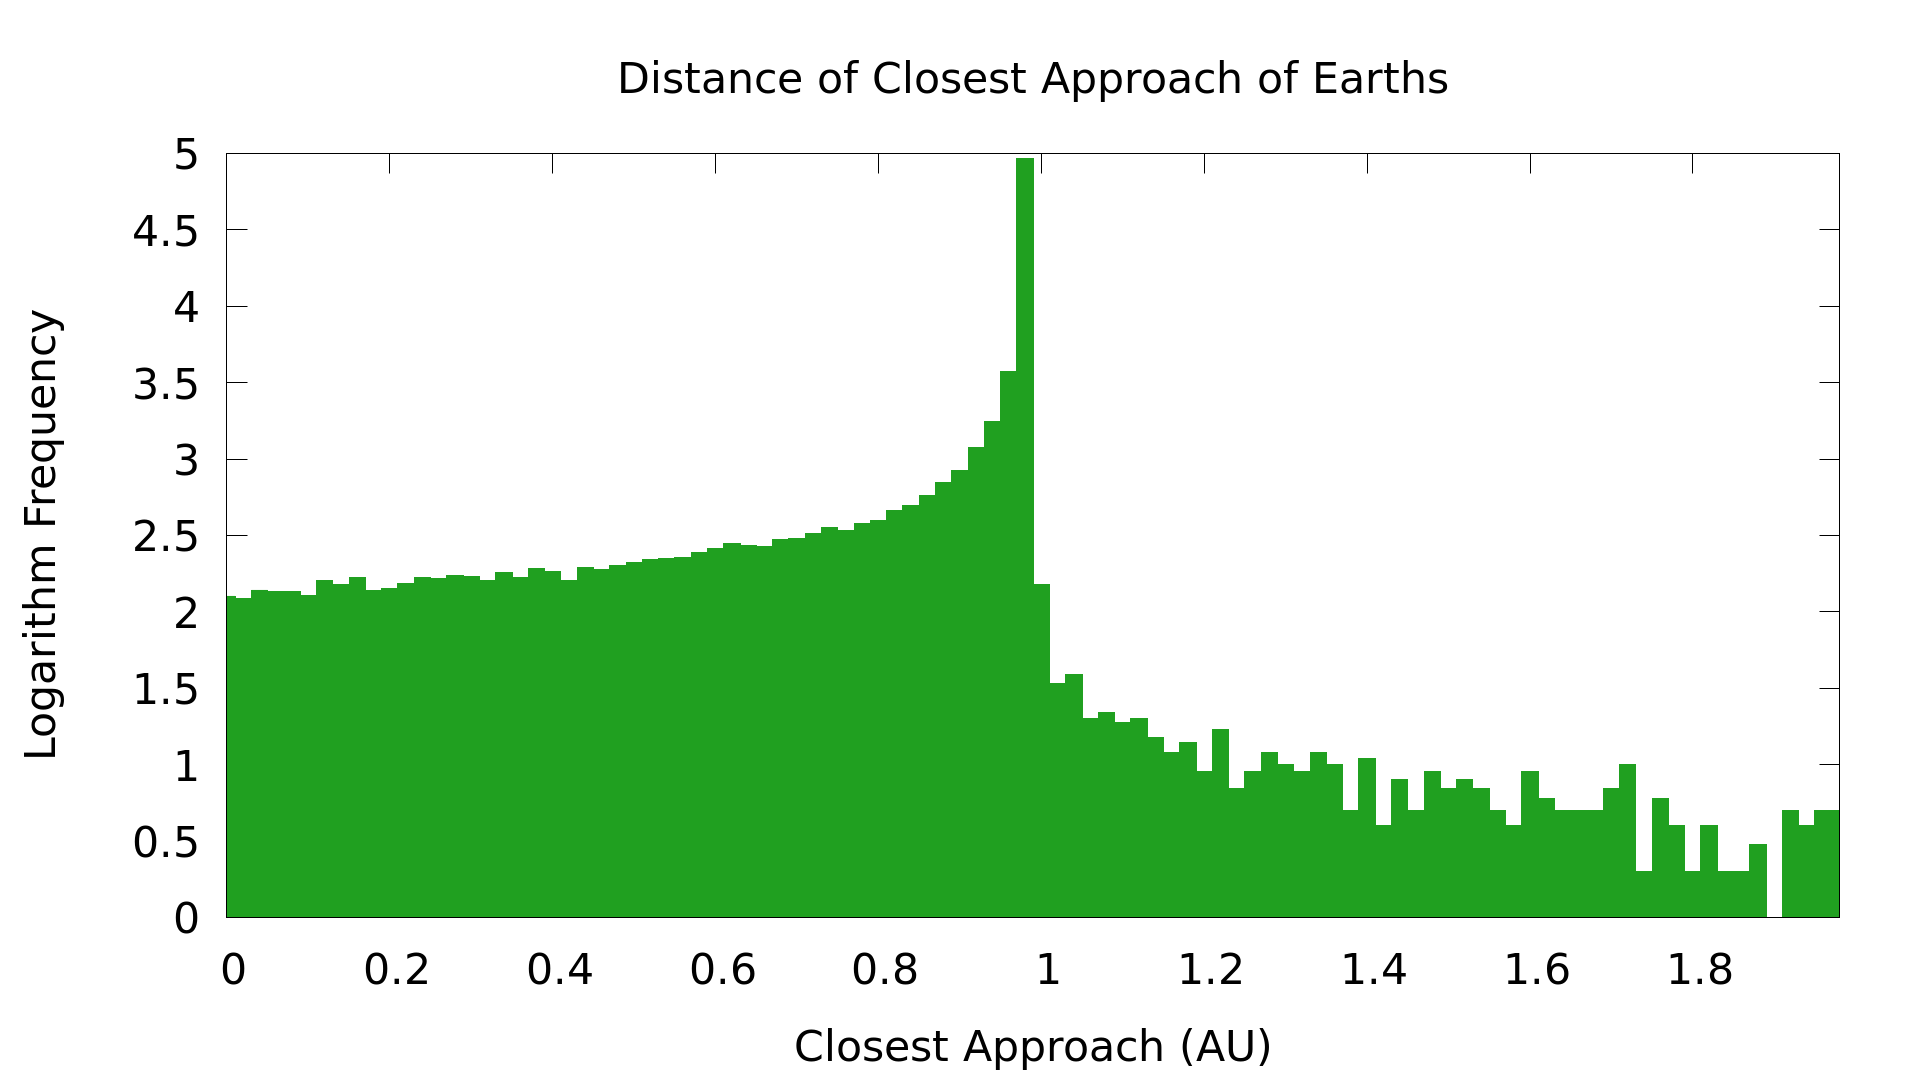
\includegraphics[height=1.20in]{periastron_earth_1000.png}
    \end{tabular}
\end{frame}

\begin{frame}{Results: Periastron, Jupiter}
    \begin{columns}
    \column{0.33\textwidth}
        \begin{itemize}
            \item Larger clusters have fewer close planets.
        \end{itemize}
    \column{0.66\textwidth}
        \begin{figure}
            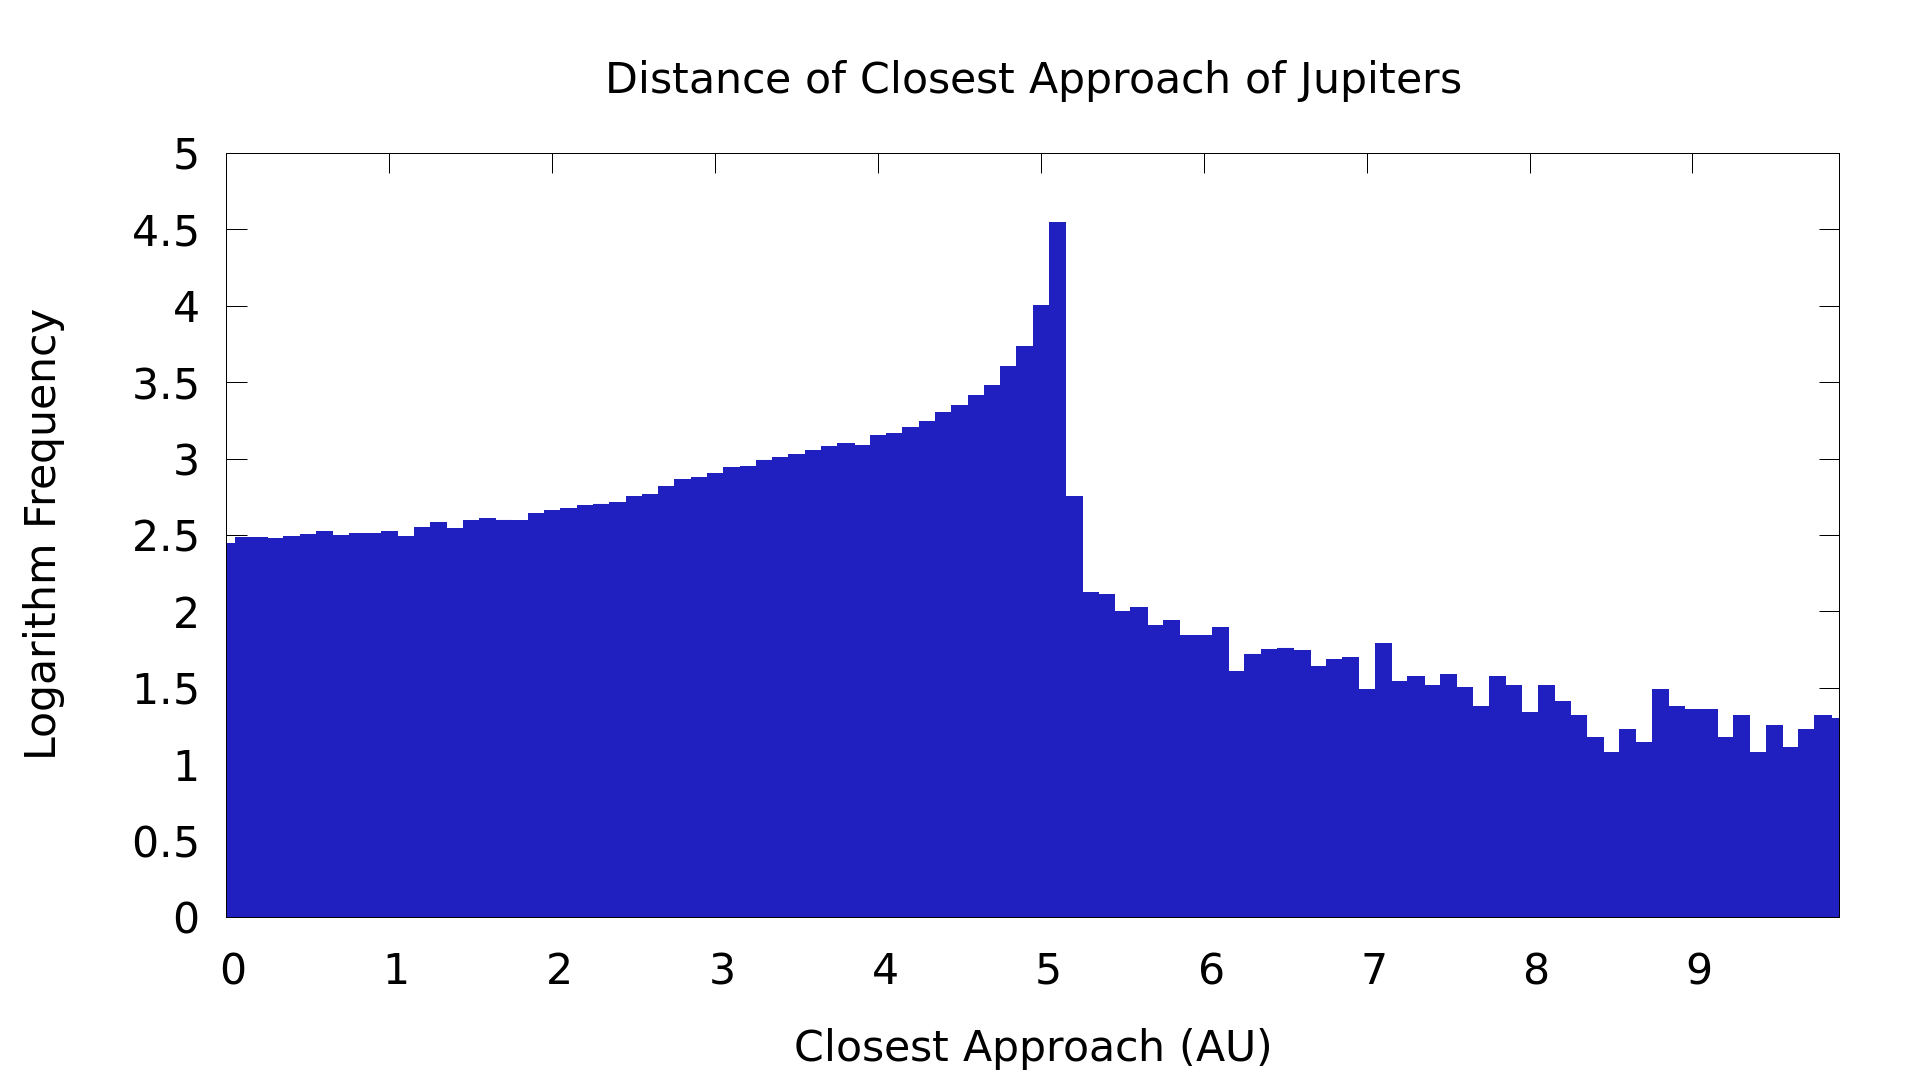
\includegraphics[height=1.20in]{periastron_jupiter_1000.png} \\
            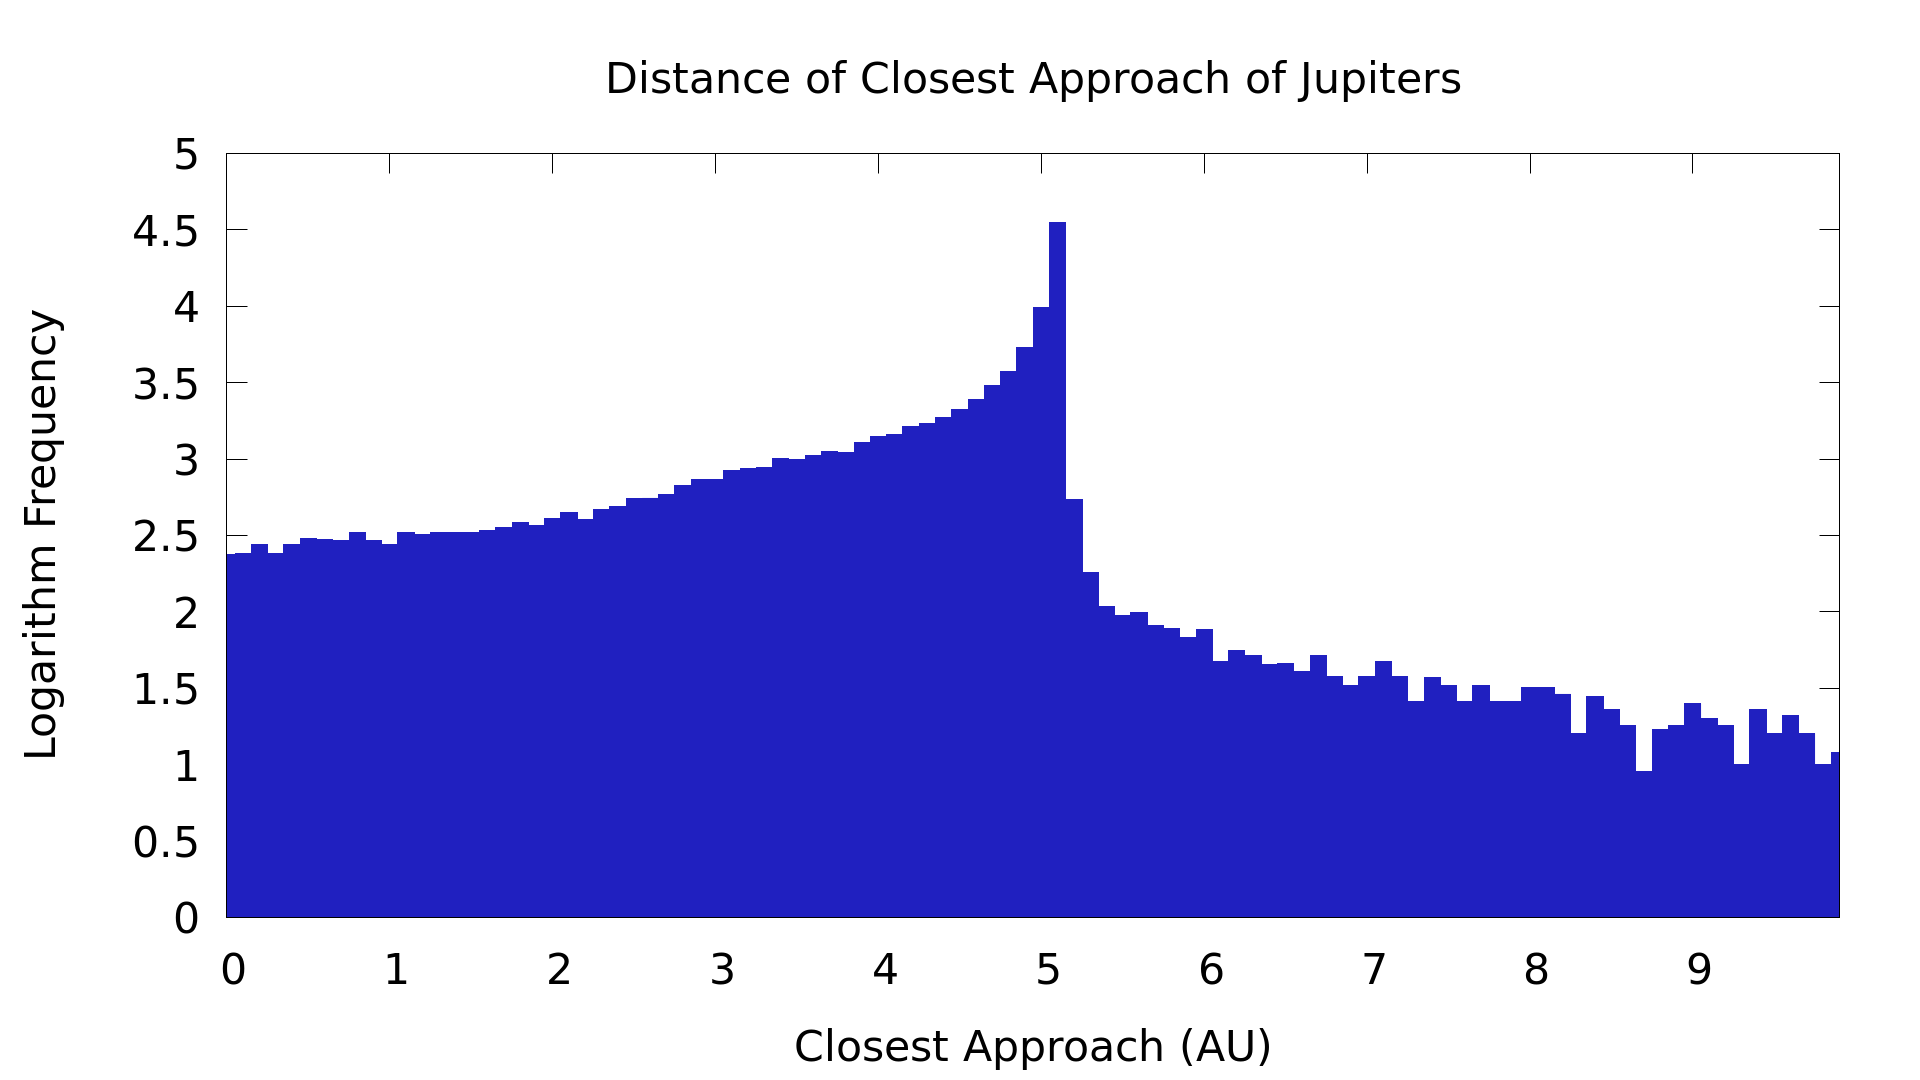
\includegraphics[height=1.20in]{periastron_jupiter_4000.png}
        \end{figure}
    \end{columns}
\end{frame}

\begin{frame}{Results: Periastron, Earth}
    \begin{columns}
    \column{0.33\textwidth}
    \column{0.66\textwidth}
        \begin{figure}
            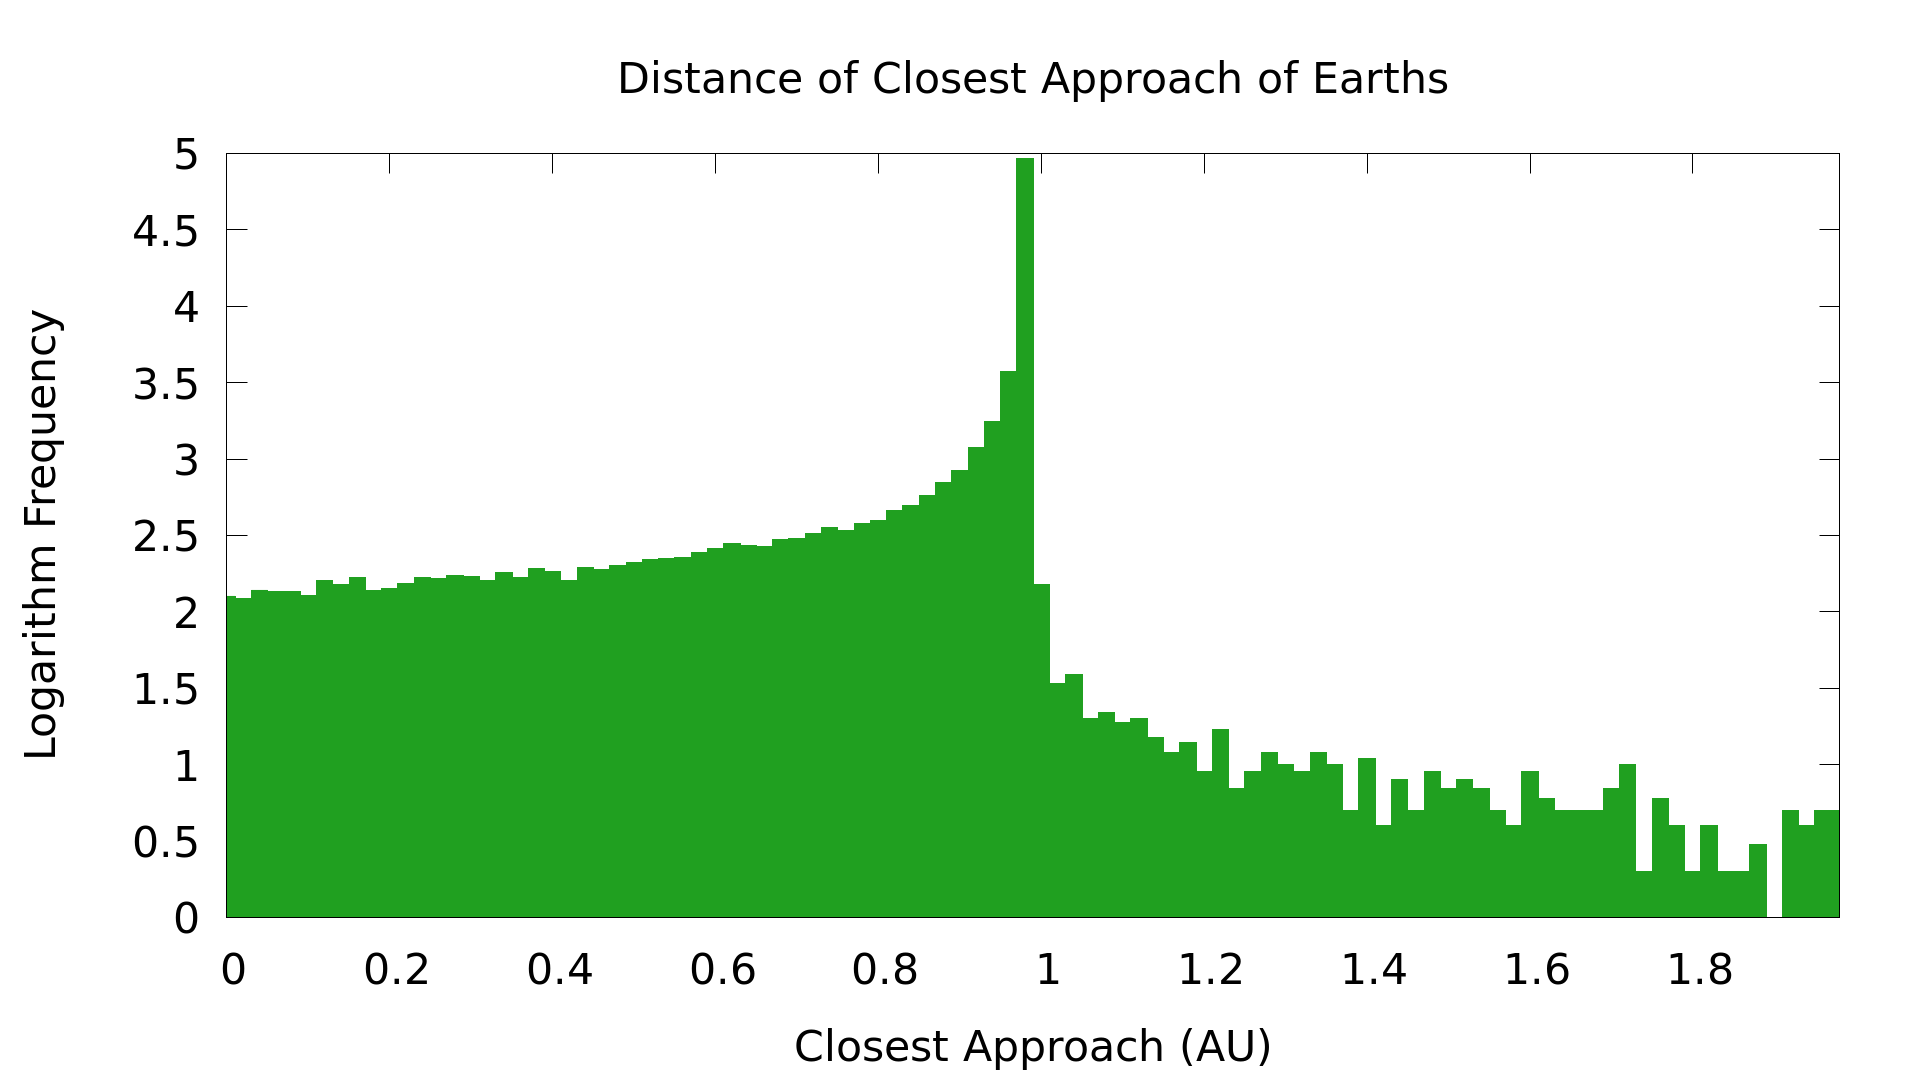
\includegraphics[height=1.20in]{periastron_earth_1000.png} \\
            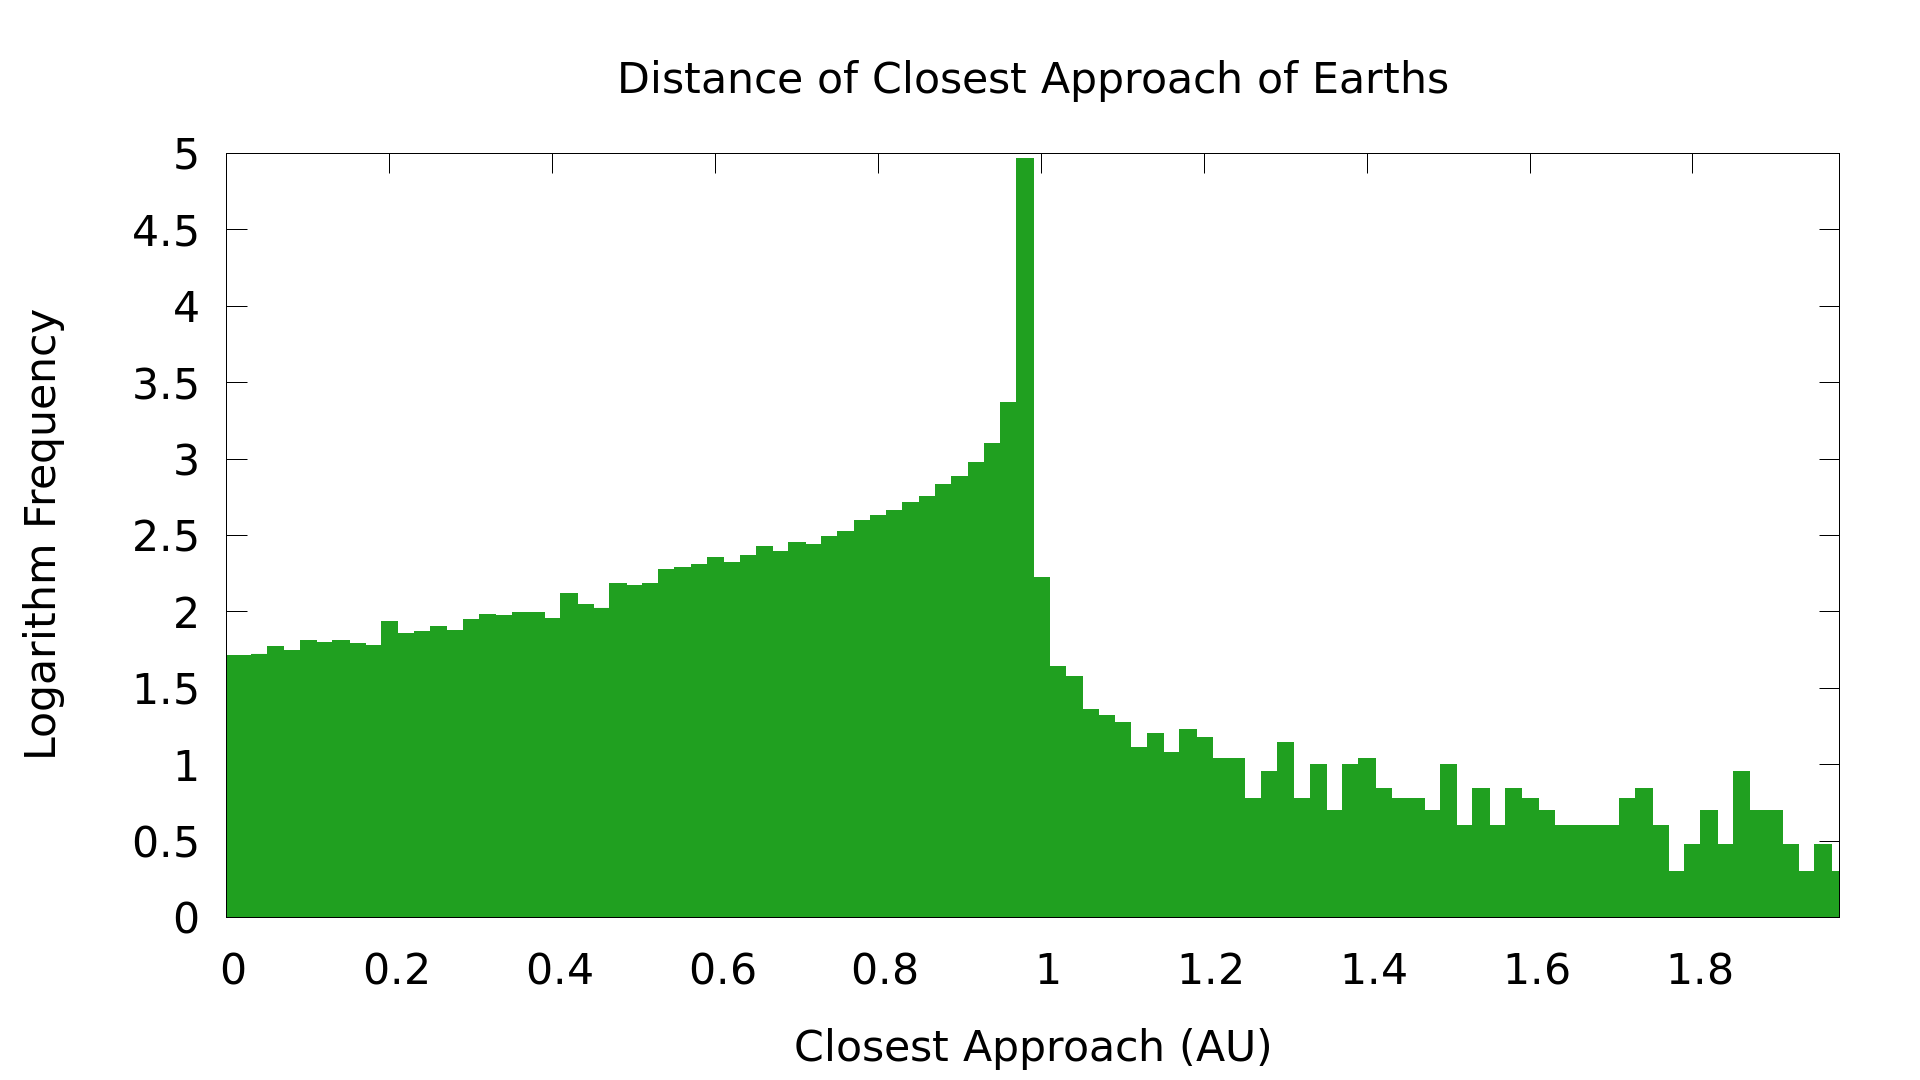
\includegraphics[height=1.20in]{periastron_earth_4000.png}
        \end{figure}
    \end{columns}
\end{frame}

\begin{frame}{Pair Planets}
    \begin{itemize}
        \item A close Jupiter greatly increases the chance of the Earth also being moved close.
    \end{itemize}
    \begin{figure}
        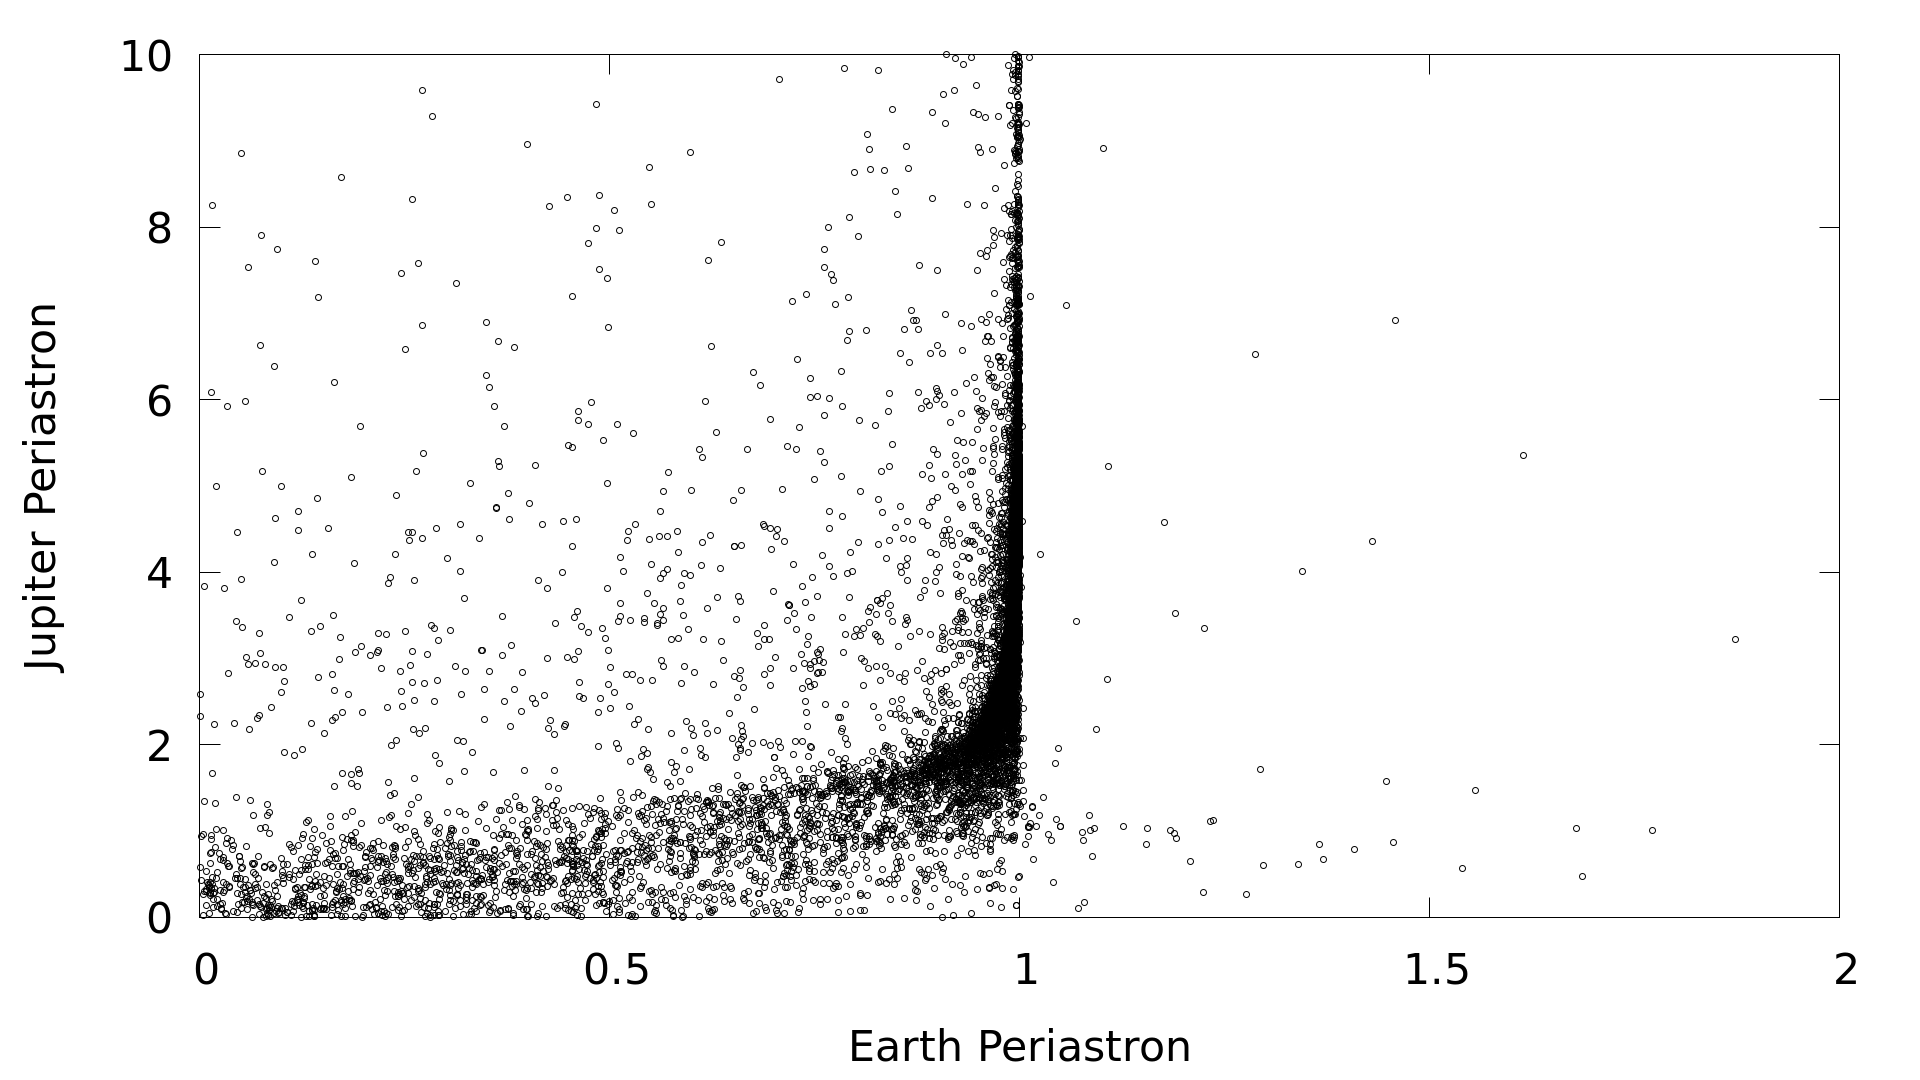
\includegraphics[height=2.20in]{evj_peri_earth_jupiter_1000.png}
    \end{figure}
\end{frame}
\begin{frame}{Pair Planets}
    \begin{itemize}
        \item This effect diminishes somewhat as the cluster size increases.
    \end{itemize}
    \begin{figure}
        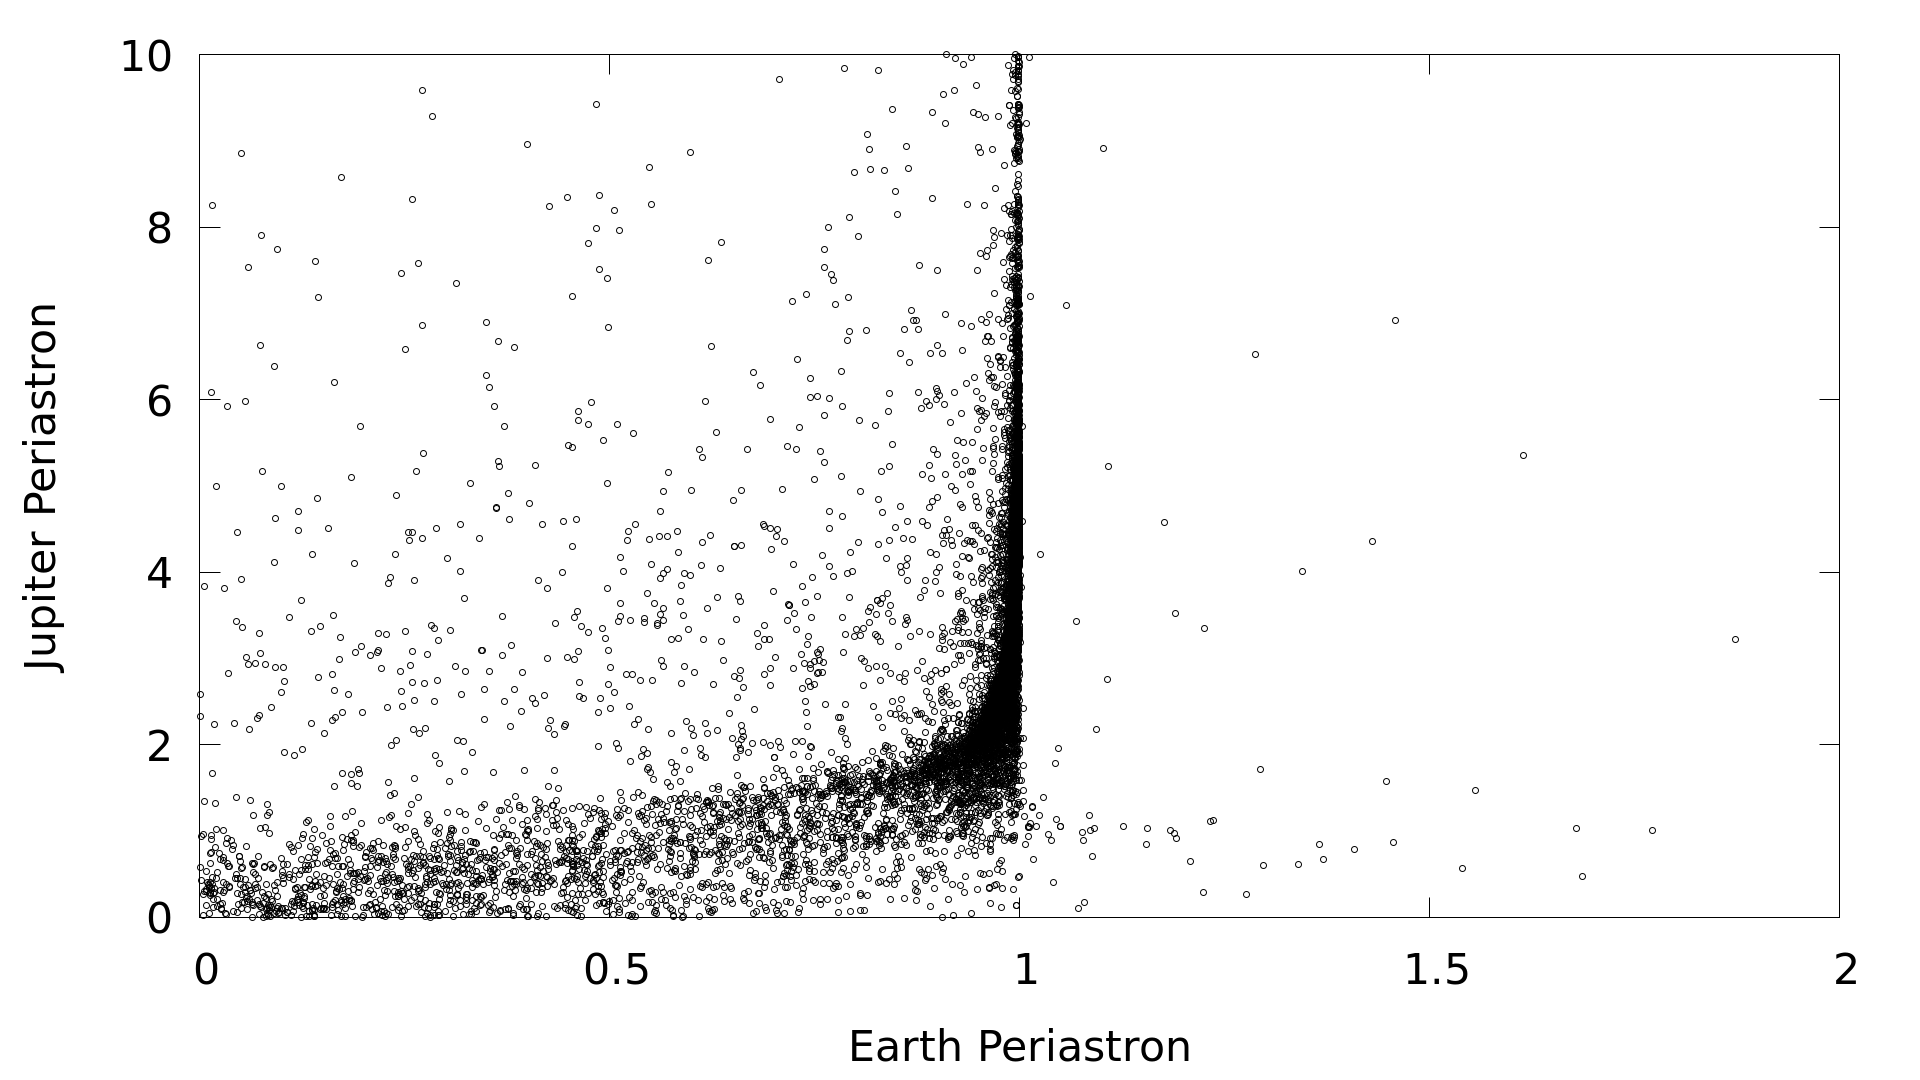
\includegraphics[height=1.00in]{evj_peri_earth_jupiter_1000.png} \\
        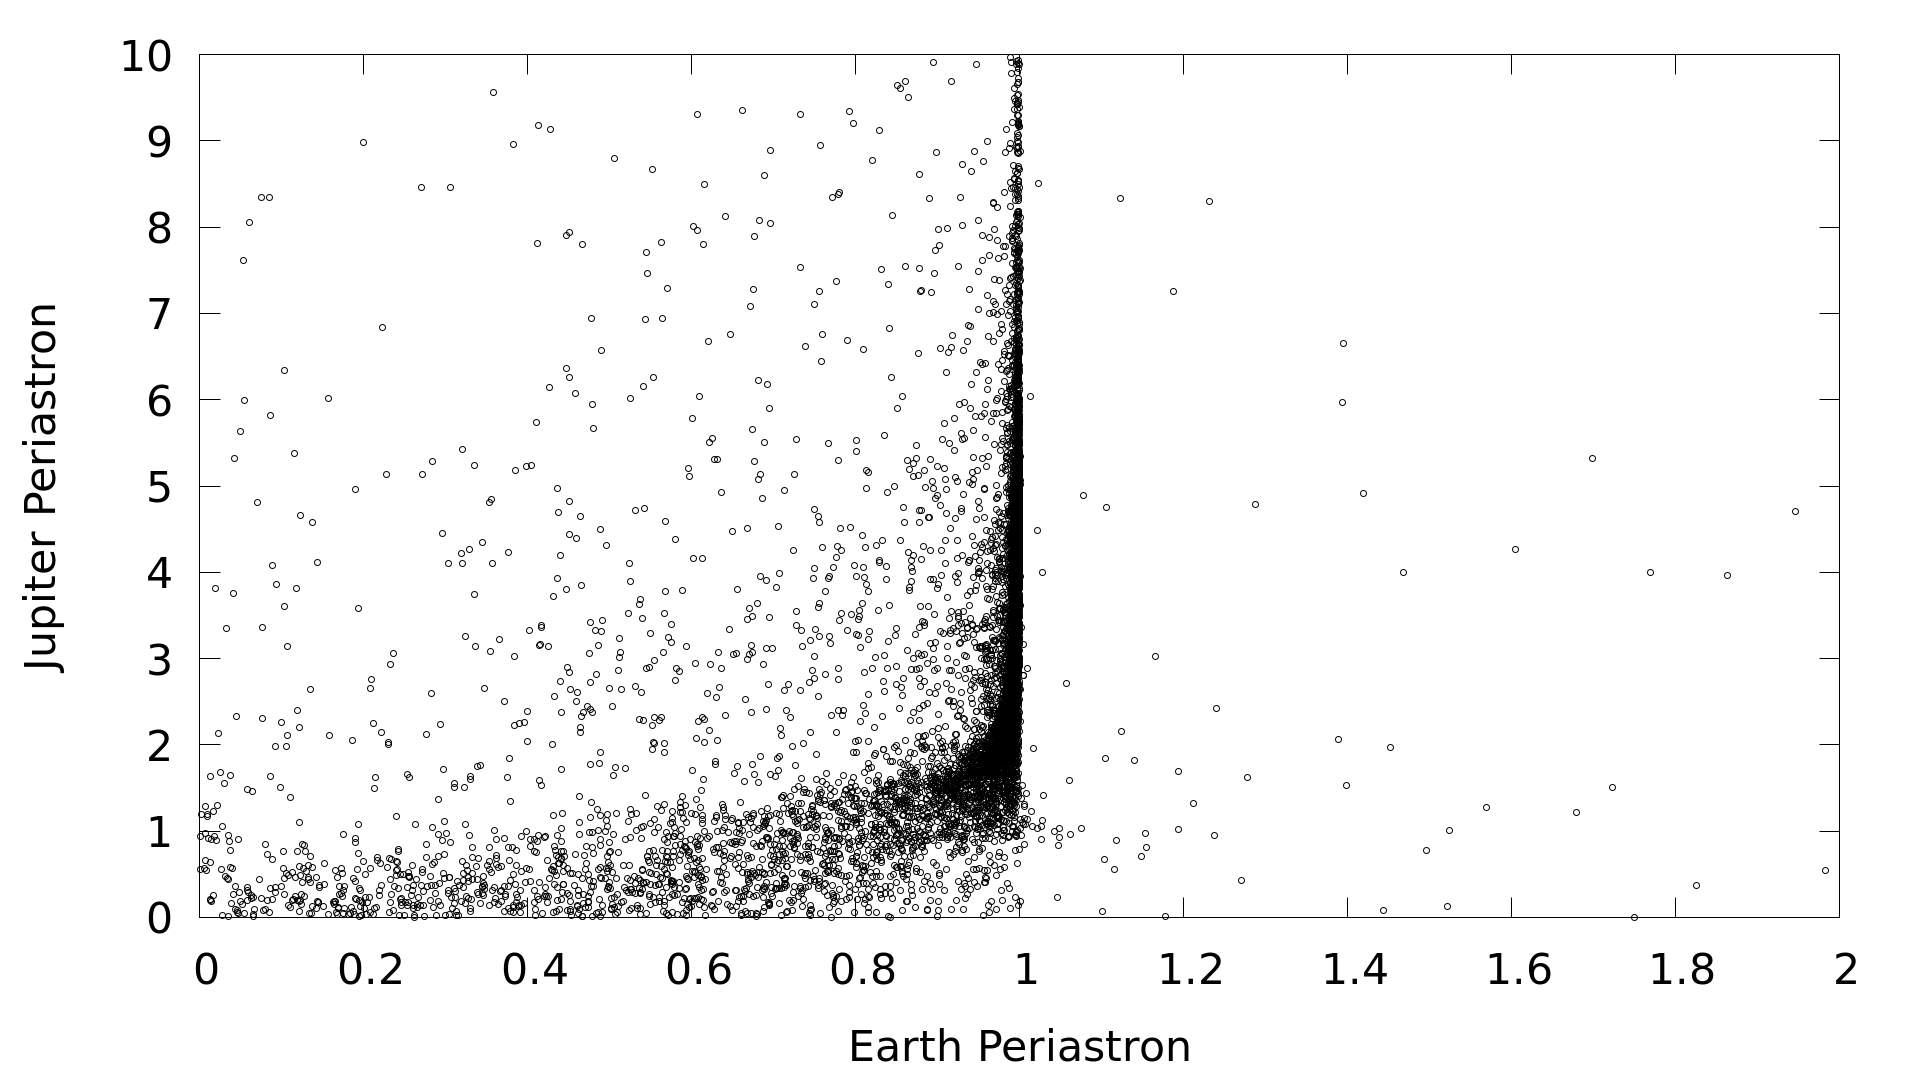
\includegraphics[height=1.00in]{evj_peri_earth_jupiter_2000.png} \\
        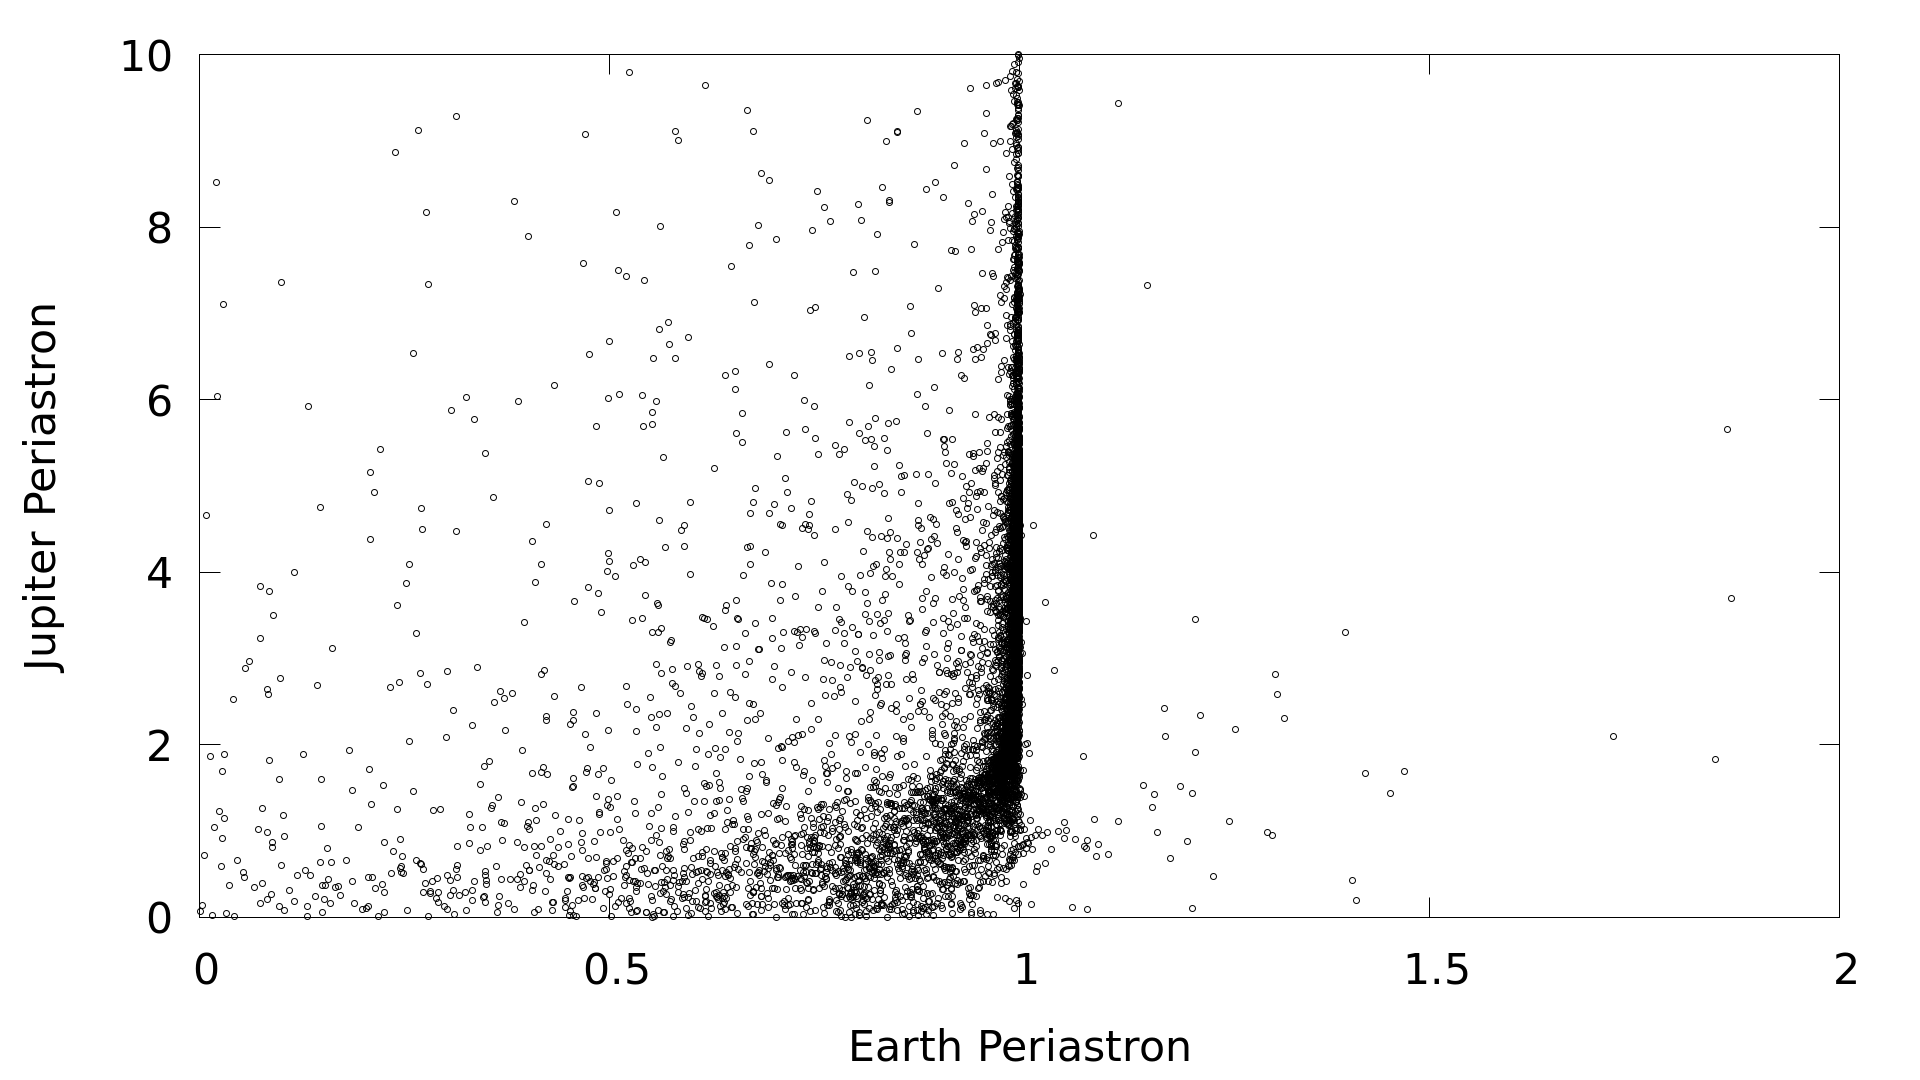
\includegraphics[height=1.00in]{evj_peri_earth_jupiter_4000.png}
    \end{figure}
\end{frame}

\begin{frame}{Pair Planets}
    \begin{itemize}
        \item An eccentric Jupiter highly increases the likelihood of Earth being eccentric.
    \end{itemize}
    \begin{figure}
        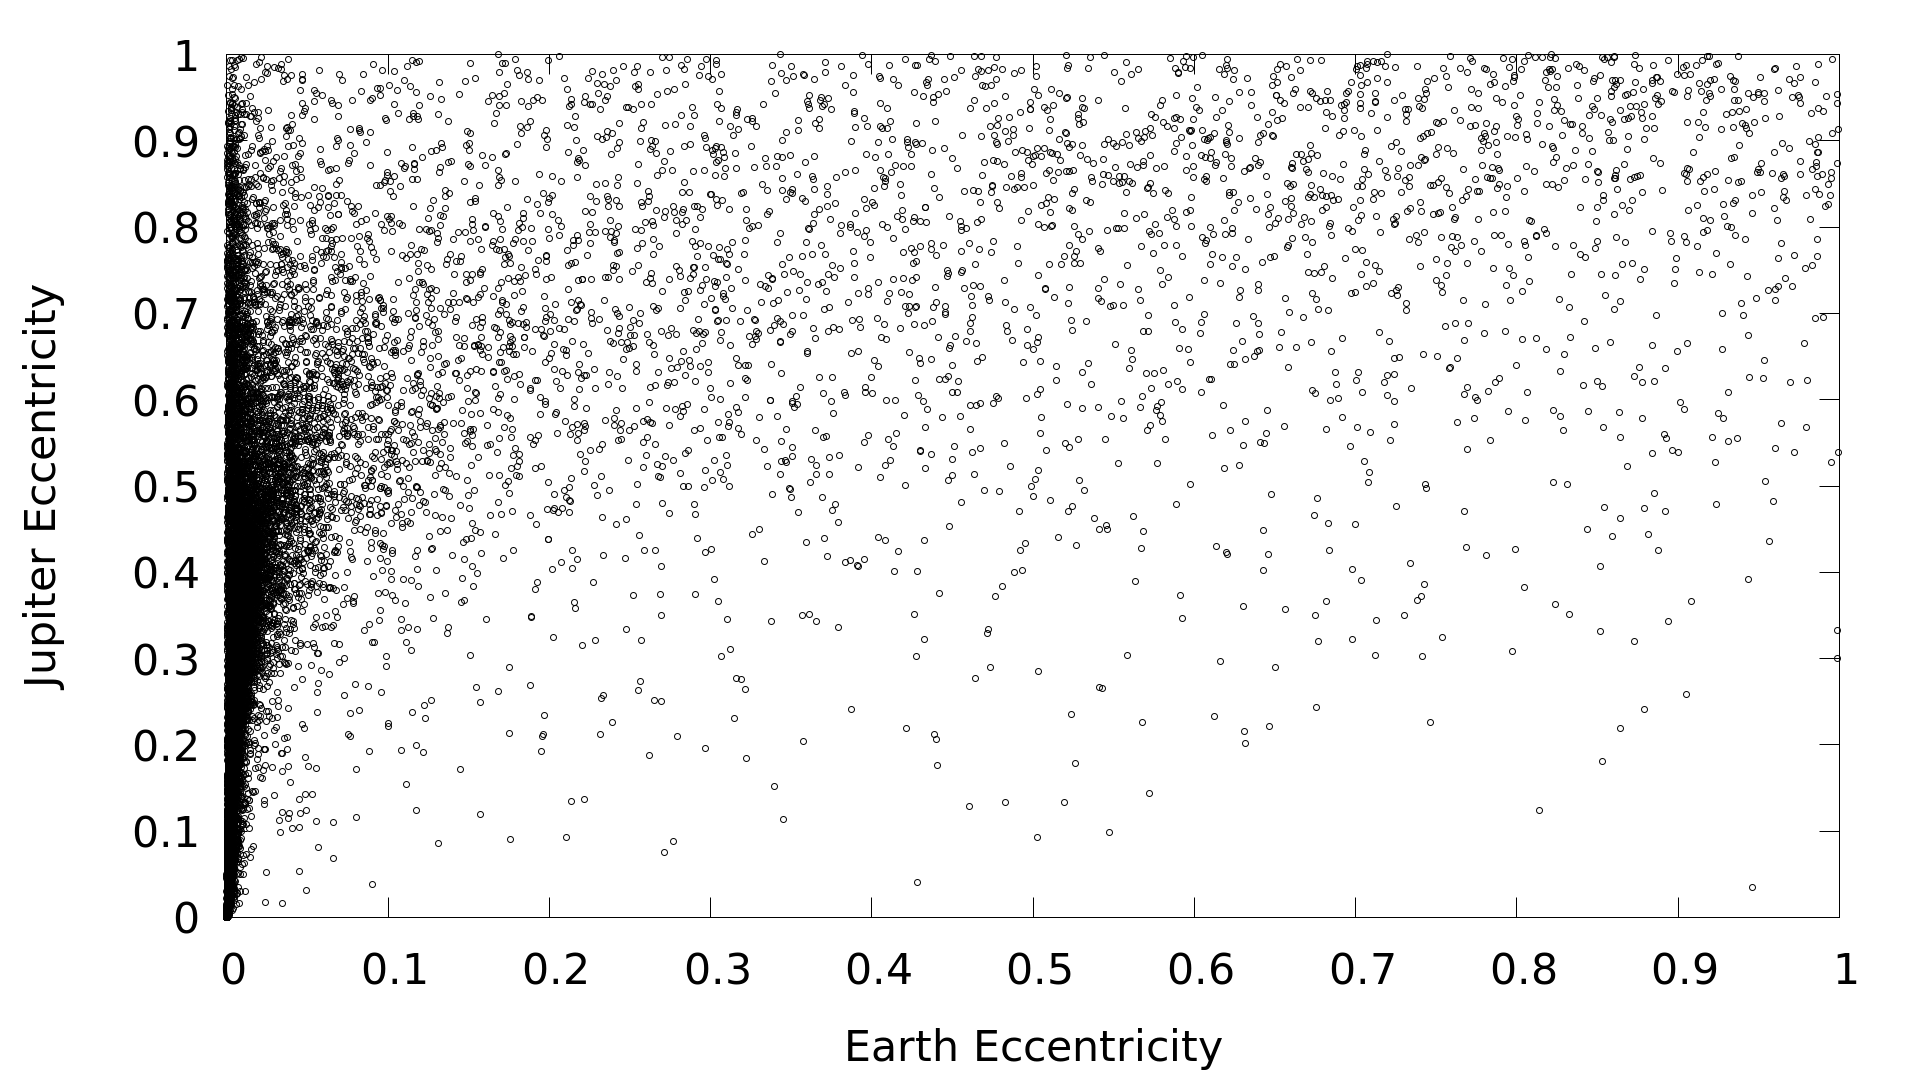
\includegraphics[height=2.20in]{evj_ecc_earth_jupiter_1000.png}
    \end{figure}
\end{frame}

\section{Conclusion}

\begin{frame}{Conclusion: Hot Jupiter Formation}
    \begin{itemize}
        \item Several hundred Jupiter planets are under 0.25 AU at closest approach.
        \item As we started with 110,000 Jupiters, the rate of occurance is between 0.1\% and 1.0\%.
        \item These Jupiters are highly eccentric.
    \end{itemize}
    \begin{figure}
        \centering
        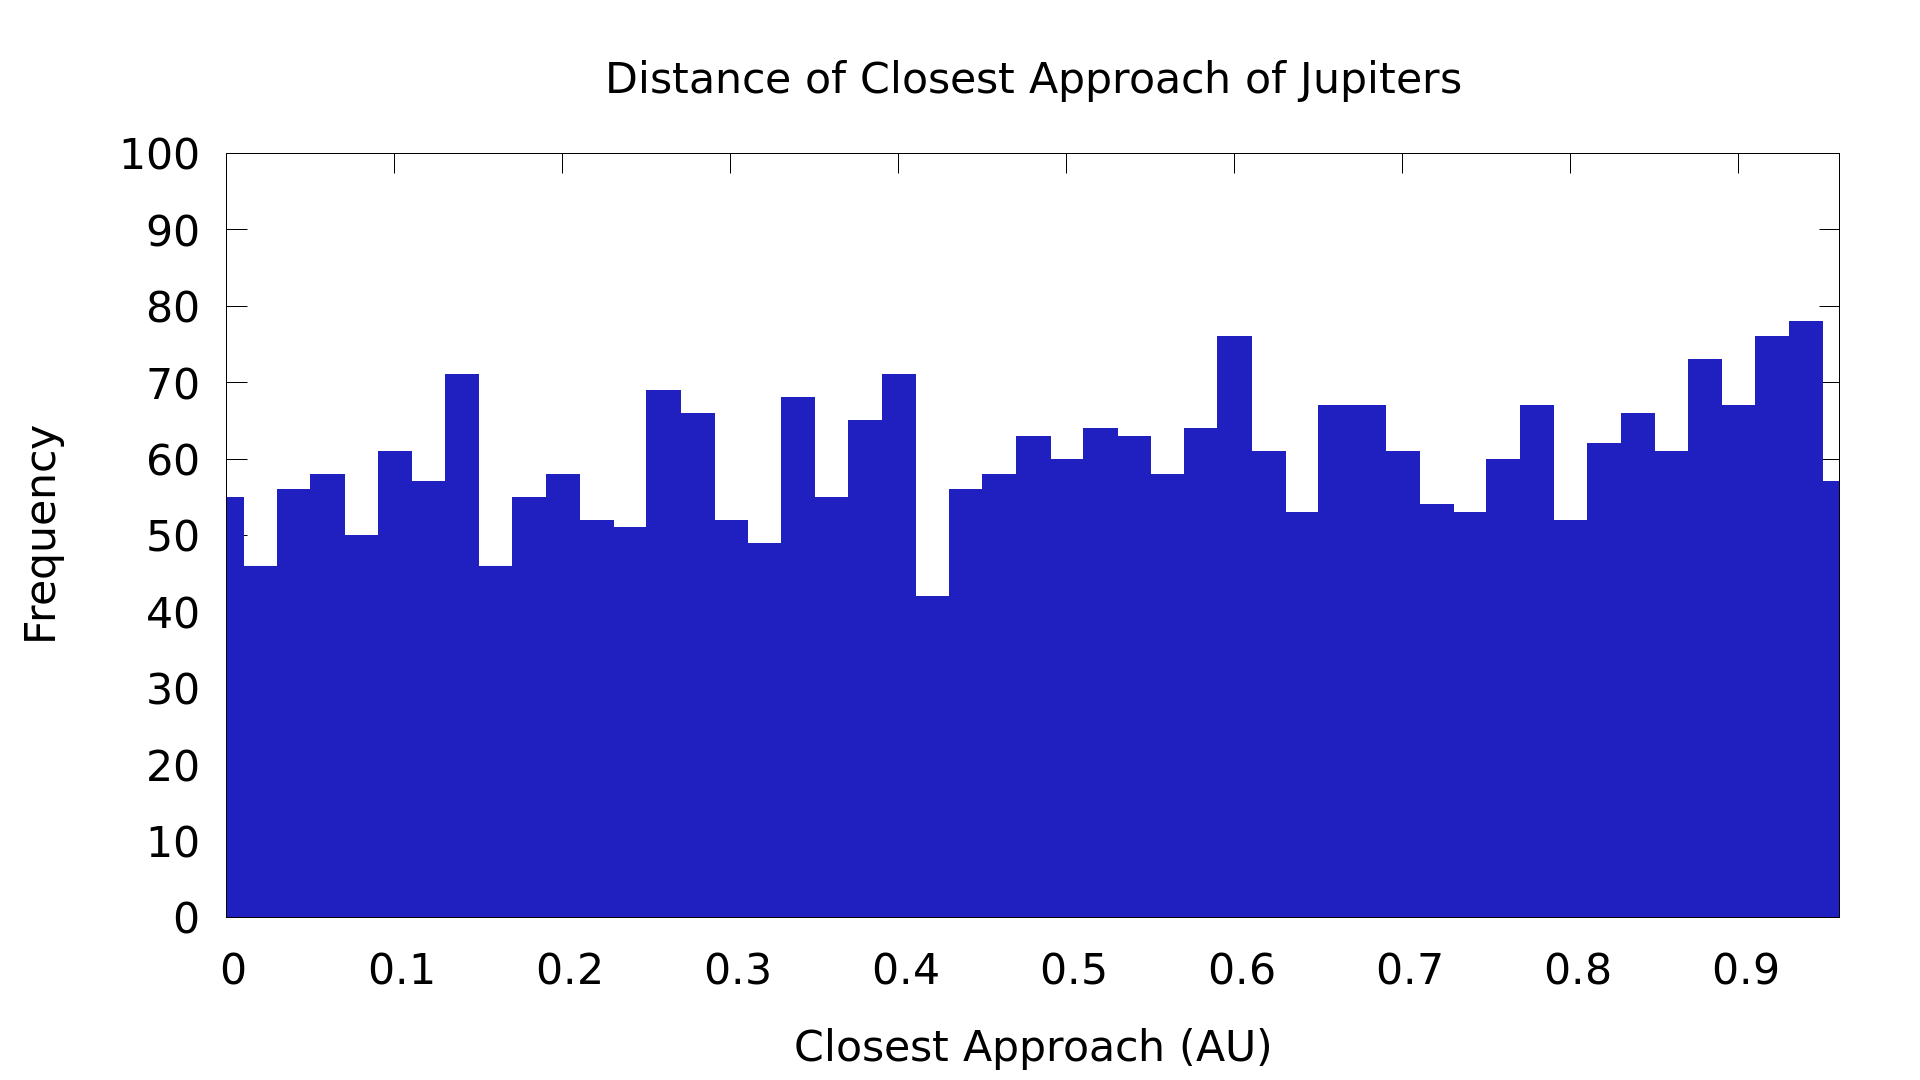
\includegraphics[height=1.85in]{periastron_jupiter_1000_close.png}
    \end{figure}
\end{frame}

\begin{frame}{Conclusion: Circularization?}
    \begin{itemize}
        \item Most Hot Jupiters are mostly circular orbits.
        \item Our simulations output eccentric Jupiters.
        \item Tidal effects on the Jupiter may "circularize" the orbit.
        \begin{itemize}
            \item This process occurs over thousands of years.
            \item Our simulation only simulates about 1,000 years for each encounter.
        \end{itemize}
        \item Further simulations need performed to determine if this can make our results
            match observation.
    \end{itemize}
\end{frame}

\begin{frame}
    \Huge
    \begin{centering}
        Questions?
    \end{centering}
\end{frame}

\end{document}
